\documentclass[12pt]{memoir}

\def\nsemestre {II}
\def\nterm {Fall}
\def\nyear {2023}
\def\nprofesor {Renzo Cavalieri}
\def\nsigla {MATH676}
\def\nsiglahead {Tropical Geometry}
\def\nlang {ENG}
%\def\darktheme{}
\let\footruleskip\relax %%FADIR

\makeatletter
\ifx \nauthor\undefined
  \def\nauthor{Ignacio Rojas}
\else
\fi

\ifx \nextra \undefined
\ifx \nlang \undefined
\author{Basado en las clases impartidas por \nprofesor \\\small Notas tomadas por \nauthor}
\else
\author{Based on the lectures by \nprofesor \\\small Notes written by \nauthor}
\fi
\else
\author{\nauthor}
\fi
\date{\nterm\ \nyear}

%%%%%%%%%%%%%
%% 1. Pacotes
%%%%%%%%%%%%%

\usepackage{alltt}
\usepackage{amsfonts}
\usepackage{amsmath}
\usepackage{amssymb}
\usepackage{amsthm}
\usepackage{algorithm}
\usepackage[noend]{algpseudocode}
\usepackage{array}
\newcommand\hmmax{0} % default 3
\newcommand\bmmax{0} % default 4 %%tex.se/3676,219310
%\usepackage{bbold}
\usepackage{bm}
\usepackage{booktabs}
%\usepackage{caption}
%\usepackage{cancel}
%\usepackage{dsfont}
\usepackage{esint}
\usepackage{fancyhdr}
\usepackage{graphicx}
\usepackage[utf8]{inputenc}
\usepackage{listings}
\usepackage{mathabx}
\usepackage[cal=euler]{mathalfa}
%\usepackage[cal=euler,frak=euler]{mathalfa} % mathcal (JIRR) precisabamos correr initexmf --mkmaps en cmd JCVDG
\usepackage{mathdots}
\usepackage{mathrsfs}
%\usepackage{mathtools}
\usepackage{microtype}
\usepackage{multicol}
\usepackage{multirow}
\usepackage[theoremfont,largesc,tighter,osf]{newpxtext} %JCV Diff
\let\widering\undefined
%\usepackage[bigdelims,vvarbb]{newpxmath} %JCVDG
%por alguna razón esto afectaba las tildes en \min, \lim y demás
%\usepackage{pdflscape}
\usepackage{pgfplots}
\usepackage{physics}
\usepackage{siunitx}
\usepackage{slashed}
%\usepackage{stmaryrd}
%\SetSymbolFont{stmry}{bold}{U}{stmry}{m}{n}
%\usepackage{subfigure}
\usepackage{subcaption}
\usepackage{tabularx}
\usepackage[breakable,skins]{tcolorbox}
\usepackage{textcomp} %%JCVDG
\usepackage{tikz}
\usepackage{tkz-euclide}
\usepackage[normalem]{ulem}
\usepackage[all]{xy}
\usepackage{imakeidx}
\ifx \nlang \undefined
\usepackage[spanish]{babel}
\else\fi 
\usepackage{wrapfig}

%%%%%%%%%%%%%%%%%%%%
%% 2. Document Setup
%%%%%%%%%%%%%%%%%%%%

\ifx \nextra \undefined
    \ifx \nlang \undefined
    \makeindex[intoc, title=Índice Analítico] %Título de índice analítico
    %El índice general es aquel en el que se indican los capítulos, títulos y subtítulos del libro.
    %Índice onomástico es donde aparece el nombre de personas mencionadas en el texto, por orden alfabético con el número de las páginas donde aparecen.
    %El índice analítico se refiere a los temas y conceptos que aparecen en el libro
    \indexsetup{othercode={\fancyhead[LE]{\emph{Índice Analítico}}}}
    \else
    \makeindex[intoc, title=Index] 
    \indexsetup{othercode={\fancyhead[LE]{\emph{Index}}}}
    \fi
  \usepackage[pdftex,
    hidelinks,
    pdfauthor={\nauthor},
    pdfsubject={Notas: \nsiglahead\ \nsemestre-\nyear},
    pdftitle={Semestre \nsemestre\ - \nsigla},
  pdfkeywords={UCR Costa Rica Matem\'aticas Mate \nsemestre\ \nterm\ \nyear\ \nsiglahead}]{hyperref}
  \title{\nsigla\ --- \nsiglahead}
\else
  \usepackage[pdftex,
     hidelinks,
    pdfauthor={\nauthor},
    pdfsubject={\nextra \nsiglahead\ \nsemestre-\nyear},
    pdftitle={Semestre \nsemestre\ - \nsigla},
  pdfkeywords={UCR Costa Rica Matem\'aticas Mate \nsemestre\ \nterm\ \nyear\ \nsiglahead\ \nextra}]{hyperref}

  \title{\nsigla\ --- \nsiglahead \\ {\Large \nextra}}
  \renewcommand\printindex{}
\fi

\pgfplotsset{compat=1.12}


\pagestyle{fancy}
\setlength{\headheight}{15.72pt} %preceding warning said make it at least this


\ifx \nsiglahead \undefined
\def\nsiglahead{\nsigla}
\fi

\lhead{} %%%empty lhead
\rfoot{\thepage}

\ifx \nextra \undefined
  \chead{
    \ifnum\thepage=1
    \else
      \ifx \nlang \undefined
      \textbf{Notas \nsiglahead\ \nsemestre-\nyear}
      \else
      \textbf{Notes \nsiglahead\ \nsemestre-\nyear}
      \fi
    \fi}
  \rhead{}%\firstxmark} % Top right header
\else
%    \chead{
%    \ifnum\thepage=1
%    \else
%      \textbf{Notas \nsiglahead\ \nsemestre-\nyear \ (\nextra)}
%    \fi}
     \chead{
       \textbf{\nextra\ \nsigla\ \nsemestre-\nyear}
     }
     \rhead{
       \textbf{\nauthor}
     }
\fi
\lfoot{}%\lastxmark} % Bottom left footer
\cfoot{} % Bottom center footer

\usetikzlibrary{arrows.meta}
\usetikzlibrary{decorations.markings}
\usetikzlibrary{decorations.pathmorphing}
\usetikzlibrary{positioning}
\usetikzlibrary{fadings}
\usetikzlibrary{intersections}
\usetikzlibrary{cd}

\ifx \nhtml \undefined
\else
  \renewcommand\printindex{}
  \DisableLigatures[f]{family = *}
  \let\Contentsline\contentsline
  \renewcommand\contentsline[3]{\Contentsline{#1}{#2}{}}
  \renewcommand{\@dotsep}{10000}
  \newlength\currentparindent
  \setlength\currentparindent\parindent

  \newcommand\@minipagerestore{\setlength{\parindent}{\currentparindent}}
  \usepackage[active,tightpage,pdftex]{preview}
  \renewcommand{\PreviewBorder}{0.1cm}

  \newenvironment{stretchpage}%
  {\begin{preview}\begin{minipage}{\hsize}}%
    {\end{minipage}\end{preview}}
  \AtBeginDocument{\begin{stretchpage}}
  \AtEndDocument{\end{stretchpage}}

  \newcommand{\@@newpage}{\end{stretchpage}\begin{stretchpage}}

  \let\@real@section\section
  \renewcommand{\section}{\@@newpage\@real@section}
  \let\@real@subsection\subsection
  \renewcommand{\subsection}{\@ifstar{\@real@subsection*}{\@@newpage\@real@subsection}}
\fi
\ifx \ntrim \undefined
\usepackage[shortlabels]{enumitem} %mfw package order matters por savetrees
\else
  \usepackage{geometry}
  \geometry{
    papersize={379pt, 699pt},
    textwidth=345pt,
    textheight=596pt,
    left=17pt,
    top=54pt,
    right=17pt
  }
  \headwidth=345pt
 \usepackage[extreme]{savetrees}
\fi

\ifx \darktheme\undefined
\else
\pagecolor[rgb]{0.2,0.231,0.302}%{0.23,0.258,0.321}
\color[rgb]{1,1,1}
\fi

\ifx \nextra \undefined
\let\@real@maketitle\maketitle
\renewcommand{\maketitle}{\@real@maketitle\begin{center}\begin{minipage}[c]{0.9\textwidth}\centering\footnotesize 
  \ifx \nlang \undefined
  Estas notas no están respaldadas por los profesores y han sido modificadas (a menudo de manera significativa) después de las clases. No están lejos de ser representaciones precisas de lo que realmente se dio en clase y en particular todos los errores son casi seguramente míos.
  \else 
  Please note that these notes were not provided or endorsed by the lecturer and have been significantly altered after the class. They may not accurately reflect the content covered in class and any errors are solely my responsibility.
  \fi
\end{minipage}\end{center}}
\else
\fi

\def\moverlay{\mathpalette\mov@rlay}
\def\mov@rlay#1#2{\leavevmode\vtop{%
   \baselineskip\z@skip \lineskiplimit-\maxdimen
   \ialign{\hfil$\m@th#1##$\hfil\cr#2\crcr}}}
\newcommand{\charfusion}[3][\mathord]{
    #1{\ifx#1\mathop\vphantom{#2}\fi
        \mathpalette\mov@rlay{#2\cr#3}
      }
    \ifx#1\mathop\expandafter\displaylimits\fi}

%%%%%%%%%%%%%%%%%%%%%%%%%%%%%%
%% 2.1 Some internal machinery
%%%%%%%%%%%%%%%%%%%%%%%%%%%%%%

\makeatletter
\renewcommand{\section}{\@startsection{section}{1}{\z@}%
							 {-3.25ex \@plus -1ex \@minus -.2ex}%
							 {1.5ex \@plus.2ex}%
							 {\normalfont\large\bfseries}}
\renewcommand{\subsection}{\@startsection{subsection}{2}{\z@}%
							 {-3.25ex \@plus -1ex \@minus -.2ex}%
							 {1.5ex \@plus .2ex}%
               {\normalfont\normalsize\bfseries}}
\newcommand*{\defeq}{\!\mathrel{\rlap{%
             \raisebox{0.3ex}{$\m@th\cdot$}}%
             \raisebox{-0.3ex}{$\m@th\cdot$}}%
                    =\!}
\makeatother
\ifx\ntrim\undefined
\newcommand{\coursetitle}{\nsigla: \nsiglahead}
\ifx\nextra\undefined
\pagestyle{ruled}
\makeoddhead{ruled}{\coursetitle}{}{\rightmark}
\else\fi
\settypeblocksize{49pc}{37pc}{*}
\setlrmargins{*}{*}{1.2}
\setulmargins{*}{*}{0.8}
\setheadfoot{16pt}{30pt}
\setheaderspaces{*}{1.5pc}{1}
\setmarginnotes{1pt}{1pt}{1pt}
\checkandfixthelayout

\setlength{\unitlength}{3pt}
\setlength{\hfuzz}{1pt}

\setlength{\fboxsep}{6pt}

\setlength{\footskip}{17pt}

\linespread{1.1}
\else\fi
\renewcommand{\cftdotsep}{\cftnodots} %%% no dots in ToC
\setpnumwidth{2em}  %%% width of page-number box in ToC


\newcommand{\stophere}{\relax} %% can be changed to `\endinput'
% \newcommand{\stophere}{\endinput} %% can be changed to `\relax'


\DeclareRobustCommand{\qned}{\ifmmode
  \else \leavevmode\unskip\penalty9999 \hbox{}\nobreak\hfill \fi
  \quad\hbox{\qnedsymbol}}
\newcommand{\qnedsymbol}{$\boxminus$} %% No-proofs end with `\qned'

\DeclareRobustCommand{\qef}{\ifmmode
  \else \leavevmode\unskip\penalty9999 \hbox{}\nobreak\hfill \fi
  \quad\hbox{\qefsymbol}}
\newcommand{\qefsymbol}{$\lozenge$} %% Examples end with `\qef'
\def\enddefn{\qef\endtrivlist}      %% `\qef' automático en defns
\def\endejem{\qef\endtrivlist}      %% `\qef' automático en ejemplos

\newcommand{\hideqed}{\renewcommand{\qed}{}} %% to suppress `\qed'
\newcommand{\hideqef}{\renewcommand{\qef}{}} %% to suppress `\qef'

% \newcommand{\ldbrack}{\ensuremath{[\mskip-2.5mu[}} %% corchetes [[
% \newcommand{\rdbrack}{\ensuremath{]\mskip-2.5mu]}} %% corchetes ]]

\newcommand{\stroke}{\mathbin|}     %% (for `\bbraket' and such)

\newcommand{\rtri}{\blacktriangleright} %% (for `\marker' and such)
\newcommand{\tribar}{|\mkern-2mu|\mkern-2mu|} %% norma triple: |||


%% Formatting changes:

\renewcommand{\labelitemi}{$\diamond$} %% instead of bullets

\renewcommand{\theenumi}{\alph{enumi}}  %% use lowercase letters
\renewcommand{\labelenumi}{\textup{(\theenumi)}} %% inside parentheses

%%%%%%%%%%%%%%
%% 2.2. Colors
%%%%%%%%%%%%%%

\definecolor{MATLABgreen}{RGB}{28,172,0} % color values Red, Green, Blue
\definecolor{MATLABlila}{RGB}{170,55,241}
\definecolor{dankBlue}{RGB}{51,60,77} % color values Red, Green, Blue
\definecolor{dankBlueLite}{RGB}{82,97,125} % color values Red, Green, Blue
\definecolor{celesUCR}{RGB}{0,192,243}
\definecolor{azulUCR}{RGB}{0,93,164}
\definecolor{verdeUCR}{RGB}{109,192,103}
\definecolor{yelloUCR}{RGB}{255,224,106}

%%%%%%%%%%%%%%%%%%%%%%%%%%%
%% 3. Theorems and suchlike
%%%%%%%%%%%%%%%%%%%%%%%%%%%

\ifx\nlang\undefined

\theoremstyle{plain}
\ifx \nextra \undefined
\newtheorem{Th}{Teorema}[section]      %%% Theorem 1.1.1
\newtheorem{Tmon}[Th]{Teoremón}
\newtheorem{Prop}[Th]{Proposición}     %%% Proposition 1.1.2
\newtheorem{Lem}[Th]{Lema}             %%% Lemma 1.1.3
\newtheorem{Cor}[Th]{Corolario}        %%% Corollary 1.1.4
\else
\newtheorem{Th}{Teorema}               %%% Theorem 1.1.1
\newtheorem{Tmon}{Teoremón}
\newtheorem{Prop}{Proposición}         %%% Proposition 1.1.2
\newtheorem{Lem}{Lema}                 %%% Lemma 3
\newtheorem{Cor}{Corolario}            %%% Corollary 4
\fi
\newtheorem*{nonum-Th}{Teorema}        %%% No-numbered Theorem
\newtheorem*{nonum-Cor}{Corolario}     %%% No-numbered Corollary

\theoremstyle{definition}
\ifx \nextra \undefined
\newtheorem{Def}[Th]{Definición}       %%% Definition 1.1.5
\newtheorem{Ex}[Th]{Ejemplo}           %%% Example 1.1.6
\newtheorem{Ej}[Th]{Ejercicio}         %%% Ejercicio 1.1.7
\else
\newtheorem{Def}{Definición}           %%% Definition 5
\newtheorem{Ex}{Ejemplo}               %%% Example 6
\newtheorem{Ej}{Ejercicio}             %%% Ejercicio 7
\fi
\newtheorem{Hec}[Th]{Hecho}            %%% Hecho 1.1.8
\newtheorem*{nonum-Def}{Definición}    %%% No number Definition
\newtheorem*{nonum-Ex}{Ejemplo}        %%% No number Example
\newtheorem*{nonum-Ej}{Ejercicio}      %%% No number Ejercicio
\newtheorem*{nonum-Hec}{Hecho}         %%% No number Fact


\theoremstyle{remark}
\newtheorem{Rmk}[Th]{Observación}      %%%Remark 1.1.9
\newtheorem*{nonum-Rmk}{Observación}         %%% No number Fact
\newtheorem*{Notn}{Notaci\'on}        %% Notaciones
\newtheorem*{Warn}{Advertencia}       %% Advertencias
\newtheorem*{Qn}{Pregunta}            %% Pregunta

\else

\theoremstyle{plain}
\ifx \nextra \undefined
\newtheorem{Th}{Theorem}[section]      %%% Theorem 1.1.1
\newtheorem{Tmon}[Th]{Teoremón}
\newtheorem{Prop}[Th]{Proposition}     %%% Proposition 1.1.2
\newtheorem{Lem}[Th]{Lemma}             %%% Lemma 1.1.3
\newtheorem{Cor}[Th]{Corollary}        %%% Corollary 1.1.4
\else
\newtheorem{Th}{Theorem}               %%% Theorem 1.1.1
\newtheorem{Tmon}{Teoremón}
\newtheorem{Prop}{Proposition}         %%% Proposition 1.1.2
\newtheorem{Lem}{Lemma}                 %%% Lemma 3
\newtheorem{Cor}{Corollary}            %%% Corollary 4
\fi
\newtheorem*{nonum-Th}{Theorem}        %%% No-numbered Theorem
\newtheorem*{nonum-Cor}{Corollary}     %%% No-numbered Corollary

\theoremstyle{definition}
\ifx \nextra \undefined
\newtheorem{Def}[Th]{Definition}       %%% Definition 1.1.5
\newtheorem{Ex}[Th]{Example}           %%% Example 1.1.6
\newtheorem{Ej}[Th]{Exercise}         %%% Exercise 1.1.7
\else
\newtheorem{Def}{Definition}           %%% Definition 5
\newtheorem{Ex}{Example}               %%% Example 6
\newtheorem{Ej}{Exercise}             %%% Exercise 7
\fi
\newtheorem{Hec}[Th]{Fact}            %%% Fact 1.1.8
\newtheorem*{nonum-Def}{Definition}    %%% No number Definition
\newtheorem*{nonum-Ex}{Example}        %%% No number Example
\newtheorem*{nonum-Ej}{Exercise}      %%% No number Exercise
\newtheorem*{nonum-Hec}{Fact}         %%% No number Fact


\theoremstyle{remark}
\newtheorem{Rmk}[Th]{Remark}      %%%Remark 1.1.9
\newtheorem*{nonum-Rmk}{Remark}         %%% No number Fact
\newtheorem*{Notn}{Notation}        %% Notaciones
\newtheorem*{Warn}{Warning}       %% Warnings
\newtheorem*{Qn}{Question}            %% Question

\fi 

\numberwithin{equation}{section}

\setlength{\parindent}{3ex}

% \renewcommand{\labelitemi}{--}
% \renewcommand{\labelitemii}{$\circ$}
% \renewcommand{\labelenumi}{(\roman{*})}

%\let\stdsection\section
%\renewcommand\section{\newpage\stdsection}

\newcommand\qedsym{\hfill\ensuremath{\square}}
% Strike through
\def\st{\bgroup \ULdepth=-.55ex \ULset}

%%%%%%%%% === My T Color Box === %%%%%%%%%%%%%%

\ifx\nlang\undefined
\ifx \darktheme\undefined
\newtcolorbox{ptcb}{
colframe = black,
colback = white,
breakable,
enhanced
}
\newtcolorbox{ptcbp}{
colframe = black,
colback = white,
coltitle = black,
colbacktitle = black!40,
title = Prueba,
breakable,
enhanced
}
\newtcolorbox{ptcbr}{
colframe = blue,
colback = white,
coltitle = blue,
colbacktitle = blue!40,
title = Respuesta,
breakable,
enhanced
}
\else
\newtcolorbox{ptcb}{
colframe = white,
colback = dankBlue,
colupper = white,
breakable,
enhanced
}
\newtcolorbox{ptcbp}{
colframe = white,
colback = dankBlue,
colupper = white,
coltitle = white,
colbacktitle = dankBlueLite,
title = Prueba,
breakable,
enhanced
}
\newtcolorbox{ptcbr}{
colframe = white,
colback = white,
coltitle = blue,
colbacktitle = blue!40,
title = Respuesta,
breakable,
enhanced
}
\fi

\else
\ifx \darktheme\undefined
\newtcolorbox{ptcb}{
colframe = black,
colback = white,
breakable,
enhanced
}
\newtcolorbox{ptcbp}{
colframe = black,
colback = white,
coltitle = black,
colbacktitle = black!40,
title = Proof,
breakable,
enhanced
}
\newtcolorbox{ptcbr}{
colframe = blue,
colback = white,
coltitle = blue,
colbacktitle = blue!40,
title = Answer,
breakable,
enhanced
}
\else
\newtcolorbox{ptcb}{
colframe = white,
colback = dankBlue,
colupper = white,
breakable,
enhanced
}
\newtcolorbox{ptcbp}{
colframe = white,
colback = dankBlue,
colupper = white,
coltitle = white,
colbacktitle = dankBlueLite,
title = Proof,
breakable,
enhanced
}
\newtcolorbox{ptcbr}{
colframe = white,
colback = white,
coltitle = blue,
colbacktitle = blue!40,
title = Answer,
breakable,
enhanced
}
\fi
\fi


%%%%%%%%% === Listings === %%%%%%%%%%%%%%
\lstset{basicstyle=\ttfamily,breaklines=true}

\lstset{language=Matlab,%
    %basicstyle=\color{red},
    breaklines=true,%
    morekeywords={matlab2tikz},
    keywordstyle=\color{blue},%
    morekeywords=[2]{1}, keywordstyle=[2]{\color{black}},
    identifierstyle=\color{black},%
    stringstyle=\color{MATLABlila},
    commentstyle=\color{MATLABgreen},%
    showstringspaces=false,%without this there will be a symbol in the places where there is a space
    numbers=left,%
    numberstyle={\tiny \color{black}},% size of the numbers
    numbersep=9pt, % this defines how far the numbers are from the text
   % emph=[1]{for,end,break,function,if,elseif,else},emphstyle=[1]\color{blue}, %some words to emphasise
    %emph=[2]{word1,word2}, emphstyle=[2]{style},
}

%%%%%%%%%%%%%%%%%%%%%%%%%%
%% 4. Simple abbreviations
%%%%%%%%%%%%%%%%%%%%%%%%%%

%%% Operator names:

\DeclareMathOperator{\area}{area}
\DeclareMathOperator{\card}{card}
\DeclareMathOperator{\ccl}{ccl}
\DeclareMathOperator{\ch}{ch}
\DeclareMathOperator{\cl}{cl}
\DeclareMathOperator{\coker}{coker}
\DeclareMathOperator{\Conv}{Conv}   %%Convex hull
\DeclareMathOperator{\cosec}{cosec}
\DeclareMathOperator{\cosech}{cosech}
\DeclareMathOperator{\covol}{covol}
\DeclareDocumentCommand\curl{}{\operatorname{curl}} 
\DeclareMathOperator{\diag}{diag}
\DeclareMathOperator{\diam}{diam}
\DeclareMathOperator{\Diff}{Diff}
\DeclareDocumentCommand\div{}{\operatorname{div}} 
\DeclareMathOperator{\energy}{energy}
\DeclareMathOperator{\erfc}{erfc}
\DeclareMathOperator{\Ext}{Ext}
\DeclareMathOperator{\fst}{fst}
\DeclareMathOperator{\Fit}{Fit}
\DeclareMathOperator{\gr}{gr}
\DeclareMathOperator{\hcf}{hcf}
\DeclareMathOperator{\Hilb}{Hilb} %Hilbert scheme
\DeclareMathOperator{\id}{id}
\DeclareMathOperator{\Ind}{Ind}
\DeclareMathOperator{\Int}{Int}
\DeclareMathOperator{\Isom}{Isom}
\DeclareMathOperator{\lcm}{lcm}
\DeclareMathOperator{\length}{length}
\DeclareMathOperator{\Lie}{Lie}
\DeclareMathOperator{\like}{like}
\DeclareMathOperator{\Lk}{Lk}
\DeclareMathOperator{\Maps}{Maps}
\DeclareMathOperator{\mcd}{mcd}
\DeclareMathOperator{\mcm}{mcm}
\DeclareMathOperator{\Min}{Min}
\DeclareMathOperator{\orb}{orb}
\DeclareMathOperator{\ord}{ord}
\DeclareMathOperator{\otp}{otp}
\DeclareMathOperator{\pr}{pr}       %% proyector
\DeclareMathOperator{\poly}{poly}
\DeclareMathOperator{\rel}{rel}
\DeclareMathOperator{\Rad}{Rad}
\DeclareMathOperator*{\res}{res}
\DeclareMathOperator{\Ric}{Ric}
\DeclareMathOperator{\rk}{rk}
\DeclareMathOperator{\Rees}{Rees}
\DeclareMathOperator{\Root}{Root}
\DeclareMathOperator{\rot}{rot}         %% rotacional
\DeclareMathOperator{\spn}{span}
\DeclareMathOperator{\St}{St}
\DeclareMathOperator{\supp}{supp}
\DeclareMathOperator{\Syl}{Syl}
\DeclareMathOperator{\Sym}{Sym}
\DeclareMathOperator{\vol}{vol}

% not-math
\newcommand{\bolds}[1]{{\bfseries #1}}
\newcommand{\cat}[1]{\mathsf{#1}}
\newcommand{\ph}{\,\cdot\,}
\newcommand{\term}[1]{\un{#1}\index{#1}}
\newcommand{\phantomeq}{\hphantom{{}={}}}
\newcommand{\ttt}{\texttt}
\newcommand{\red}[1]{\textcolor{red}{#1}}
\newcommand{\prp}[1]{\textcolor{purple}{#1}}
\newcommand{\blu}[1]{\textcolor{azulUCR}{#1}}
\newcommand{\green}[1]{\textcolor{verdeUCR}{#1}}
\newcommand{\yelo}[1]{\textcolor{yelloUCR}{#1}}
\newcommand{\cele}[1]{\textcolor{celesUCR}{#1}}

%functions
\DeclareMathOperator{\sgn}{sgn}
\newcommand*{\Cdot}{{\raisebox{-0.25ex}{\scalebox{1.5}{$\cdot$}}}}      %% cdot más grande
\newcommand{\ind}{\mathbf{1}}       %%%indicator function
\newcommand{\mm}{\mathfrak{m}}      %%%metric


% Greek letters:

\newcommand{\al}{\alpha}                %% short for  \alpha
\newcommand{\bt}{\beta}                 %% short for  \beta
\newcommand{\Dl}{\Delta}                %% short for  \Delta
\newcommand{\dl}{\delta}                %% short for  \delta
\newcommand{\eps}{\varepsilon}          %% short for  \varepsilon
\newcommand{\Ga}{\Gamma}                %% short for  \Gamma
\newcommand{\ga}{\gamma}                %% short for  \gamma
\newcommand{\kp}{\kappa}                %% short for  \kappa
\newcommand{\La}{\Lambda}               %% short for  \Lambda
\newcommand{\la}{\lambda}               %% short for  \lambda
\newcommand{\Om}{\Omega}                %% short for  \Omega
\newcommand{\om}{\omega}                %% short for  \omega
\newcommand{\Sg}{\Sigma}                %% short for  \Sigma
\newcommand{\sg}{\sigma}                %% short for  \sigma
\newcommand{\Te}{\Theta}                %% short for  \Theta
\newcommand{\te}{\theta}                %% short for  \theta
\newcommand{\ups}{\upsilon}             %% short for  \upsilon
\newcommand{\vf}{\varphi}               %% short for  \varphi
\newcommand{\ze}{\zeta}                 %% short for  \zeta
\newcommand{\vsg}{\varsigma}            %% short for  \varsigma
\newcommand{\vte}{\vartheta}            %% short for  \vartheta

%Boldface letters

\newcommand{\bA}{\mathbb{A}}        %% antisimetrizador
\newcommand{\bB}{\mathbb{B}}        %% bola unitaria
\newcommand{\bC}{\mathbb{C}}    %%% números complejos
\newcommand{\bCP}{\mathbb{CP}}  %%% espacio proyectivo complejo
\newcommand{\bD}{\mathbb{D}}        %% Poincaré disk
\newcommand{\bE}{\mathbb{E}}
\newcommand{\bF}{\mathbb{F}}        %% un cuerpo
\newcommand{\bH}{\mathbb{H}}        %% cuaterniones
\newcommand{\bI}{\mathbb{I}}        %% ideal de zeros
\newcommand{\bK}{\mathbb{K}}            %% ein korper
\newcommand{\bN}{\mathbb{N}}    %%% números naturales
\newcommand{\bP}{\mathbb{P}}        %% números enteros positivos
\newcommand{\bQ}{\mathbb{Q}}    %%% números racionales
\newcommand{\bR}{\mathbb{R}}    %%% números reales
\newcommand{\bRP}{\mathbb{RP}}  %%% espacio proyectivo real
\newcommand{\bS}{\mathbb{S}}    %%% esfera
\newcommand{\bT}{\mathbb{T}}        %% círculo o toro
\newcommand{\bV}{\mathbb{V}}        %% lugar geométrico de ceros
\newcommand{\bZ}{\mathbb{Z}}    %%% números enteros

%Script letters:

\newcommand{\cA}{\mathcal{A}}           %% formas diferenciales
\newcommand{\cB}{\mathcal{B}}           %% una base vectorial
\newcommand{\cC}{\mathcal{C}}           %% otra base vectorial
\newcommand{\cD}{\mathcal{D}}           %% funciones de prueba
\newcommand{\cE}{\mathcal{E}}           %% un modulo proyectivo
\newcommand{\cF}{\mathcal{F}}           %% espacio de Fock
\newcommand{\cG}{\mathcal{G}}           %% funtor de Gelfand
\newcommand{\cH}{\mathcal{H}}           %% espacio de Hilbert
\newcommand{\cI}{\mathcal{I}}           %% un funtor de inclusion
\newcommand{\cJ}{\mathcal{J}}           %% otro funtor
\newcommand{\cK}{\mathcal{K}}           %% otro espacio de Hilbert
\newcommand{\cL}{\mathcal{L}}           %% operadores lineales
\newcommand{\cM}{\mathcal{M}}           %% multiplicadores
\newcommand{\cN}{\mathcal{N}}           %% funciones nulas
\newcommand{\cO}{\mathcal{O}}           %% funciones de crec-to lento
\newcommand{\cP}{\mathcal{P}}           %% una particion
\newcommand{\cR}{\mathcal{R}}           %% funciones representativas
\newcommand{\cQ}{\mathcal{Q}}           %% otra particion
\newcommand{\cS}{\mathcal{S}}           %% funciones de Schwartz
\newcommand{\cT}{\mathcal{T}}           %% una topologia
\newcommand{\cU}{\mathcal{U}}           %% cubrimiento abierto
\newcommand{\cV}{\mathcal{V}}           %% vecindarioas
\newcommand{\cW}{\mathcal{W}}           %% grupo de Weyl
\newcommand{\cZ}{\mathcal{Z}}           %% topología de Zariski

%%% Fraktur letters:

\newcommand{\gA}{\mathfrak{A}}      %% un atlas
\newcommand{\g}{\mathfrak{g}}       %% un álgebra de Lie
\newcommand{\gB}{\mathfrak{B}}      %% otro atlas
\newcommand{\ggl}{\mathfrak{gl}}    %% álg de Lie general lineal
\newcommand{\gsl}{\mathfrak{sl}}    %% álg de Lie especial lineal
\newcommand{\gso}{\mathfrak{so}}    %% álg de Lie especial ortogonal
\newcommand{\gsu}{\mathfrak{su}}    %% álg de Lie especial unitaria
\newcommand{\gX}{\mathfrak{X}}      %% campos vectoriales

%%% Roman letters:

\newcommand{\dR}{\mathrm{dR}}       %% cohomología de de Rham
\newcommand{\rGL}{\mathrm{GL}}      %% grupo general lineal
\newcommand{\rO}{\mathrm{O}}        %% grupo ortogonal
\newcommand{\rSL}{\mathrm{SL}}      %% grupo especial lineal
\newcommand{\rSO}{\mathrm{SO}}      %% grupo ortogonal especial
\newcommand{\rSp}{\mathrm{Sp}}      %% grupo simpléctico
\newcommand{\rSU}{\mathrm{SU}}      %% grupo unitario especial
\newcommand{\rU}{\mathrm{U}}        %% grupo unitario
\newcommand{\rUH}{\mathrm{UH}}      %% cuaterniones unitarias
\newcommand{\rT}{\mathrm{T}}        %% grupo triangular

% Sanserif letters:

\newcommand{\sA}{\mathsf{A}}            %% algebras de Lie A_n
\newcommand{\sB}{\mathsf{B}}            %% grupo como categoria
\newcommand{\sC}{\mathsf{C}}            %% una categoria
\newcommand{\sD}{\mathsf{D}}            %% otra categoria
\newcommand{\sE}{\mathsf{E}}            %% otra categoria mas
\newcommand{\sF}{\mathsf{F}}            %% algebra de Lie F_4
\newcommand{\sG}{\mathsf{G}}            %% algebra de Lie G_2
\newcommand{\sJ}{\mathsf{J}}            %% un poset
\newcommand{\sK}{\mathsf{K}}            %% un poset
\newcommand{\sL}{\mathcal{L}}           %% derivada de Lie
\newcommand{\sN}{\mathsf{N}}            %% categoría con objetos \bN
\newcommand{\sT}{\mathsf{T}}            %% transpuesta

%%% Boldface letters:

\bmdefine{\CC}{C}                       %% C negrilla
\bmdefine{\cc}{c}
%\bmdefine{\dd}{d}                       %% d negrilla
\bmdefine{\ee}{e}                       %% vector e
\bmdefine{\eeps}{\varepsilon}           %% basic form \eps
\bmdefine{\FF}{F}                       %% vector F
\bmdefine{\ff}{f}                       %% vector f
\bmdefine{\ii}{i}                       %% cuaternion i
\bmdefine{\jj}{j}                       %% cuaternion j
\bmdefine{\kk}{k}                       %% cuaternion k
\bmdefine{\lla}{\lambda}                %% sucesion \la
\bmdefine{\mmu}{\mu}                    %% sucesion \mu
\bmdefine{\pp}{p}                       %% vector p
\bmdefine{\qq}{q}                       %% vector q
\bmdefine{\rr}{r}                       %% vector r
\bmdefine{\ssg}{\sigma}                 %% vector \sg
%\bmdefine{\sss}{s}
%\bmdefine{\ttt}{t}
\bmdefine{\VV}{V}                       %% V negrilla
\bmdefine{\xx}{x}                       %% sucesion x
\bmdefine{\xxi}{\xi}                    %% vector \xi
\bmdefine{\yy}{y}                       %% sucesion y
\bmdefine{\zz}{z}                       %% sucesion z

% Matrix groups
\DeclareMathOperator{\GL}{GL}   %%% grupo general lineal
\DeclareMathOperator{\Or}{O}    %%% grupo ortogonal
\DeclareMathOperator{\PGL}{PGL} %%% grupo proyectivo lineal
\DeclareMathOperator{\PSL}{PSL} %%% grupo proyectivo lineal especial
\DeclareMathOperator{\PSO}{PSO} %%% grupo proyectivo ortogonal
\DeclareMathOperator{\PSU}{PSU} %%% grupo proyectivo unitario
\DeclareMathOperator{\SL}{SL}   %%% grupo especial lineal
\DeclareMathOperator{\SO}{SO}   %%% grupo especial ortogonal
\DeclareMathOperator{\SU}{SU}   %%% grupo especial unitario

% Numericc
\newcommand{\argmin}{\text{argm\'in}}
\DeclareMathOperator{\dof}{dof}

%% Brackets
\newcommand{\conj}[1]{\left\lbrace#1\right\rbrace}
\newcommand{\bonj}[1]{\left\lbrack#1\right\rbrack}
\newcommand{\obonj}[1]{\left\rbrack#1\right\lbrack}
\newcommand{\rbonj}[1]{\left\rbrack#1\right\rbrack}
\newcommand{\lbonj}[1]{\left\lbrack#1\right\lbrack}
\newcommand{\snm}[1]{\|#1\|}           %small norma
\newcommand{\nm}[1]{\left\|#1\right\|} %norma pegadita
\newcommand{\pnm}[1]{\biggl|\biggl|#1\biggr|\biggr|}
\let\oldvec=\vec
\renewcommand{\vec}[1]{\mathbf{#1}}
\newcommand\quot[2]{
        \mathchoice
            {% \displaystyle
                \text{\raise1ex\hbox{$#1$}\Big/\lower1ex\hbox{$#2$}}%
            }
            {% \textstyle
                {^{ #1}/_{ #2}}
            }
            {% \scriptstyle
                {^{ #1}/_{ #2}}
            }
            {% \scriptscriptstyle
                {^{ #1}/_{ #2}}
            }
    }
%\newcommand*\quot[2]{{^{\textstyle #1}\big/_{\textstyle #2}}}
\newcommand*\squot[2]{{^{ #1}/_{ #2}}}%%%small quotient
\newcommand{\multinom}[2]{\ensuremath{\left(\kern-.3em\left(\genfrac{}{}{0pt}{}{#1}{#2}\right)\kern-.3em\right)}}

% Probability
\DeclareMathOperator{\Bernoulli}{Bernoulli}
\DeclareMathOperator{\betaD}{beta}
\DeclareMathOperator{\bias}{bias}
\DeclareMathOperator{\binomial}{binomial}
\DeclareMathOperator{\corr}{corr}
\DeclareMathOperator{\cov}{cov}
\DeclareMathOperator{\gammaD}{gamma}
\DeclareMathOperator{\mse}{mse}
\DeclareMathOperator{\multinomial}{multinomial}
\DeclareMathOperator{\Poisson}{Poisson}
\DeclareMathOperator{\Var}{Var}     %%%variance
\DeclareMathOperator{\Cov}{Cov}     %%%Covariance
\renewcommand{\mid}{\;\ifnum\currentgrouptype=16 \middle\fi|\;}

% Combinatorics
\DeclareMathOperator{\ins}{ins}   % insertion tableaux
\DeclareMathOperator{\asc}{asc}   % ascents
\DeclareMathOperator{\rw}{rw}     % reading word
\DeclareMathOperator{\rev}{rev}     % reading word
\DeclareMathOperator{\rect}{rect} % rectification of young tableau
\DeclareMathOperator{\sh}{sh}     % shape of young tableau
\DeclareMathOperator{\std}{std}   % standarization
\DeclareMathOperator{\Fl}{\mathcal{F}\ell}       %% conjunto de Flags
\DeclareMathOperator{\Frob}{Frob} % Frobenius map

% Algebra
\DeclareMathOperator{\Ad}{Ad}       %% acción adjunta
\DeclareMathOperator{\adj}{adj}
\DeclareMathOperator{\Ann}{Ann}     %% aniquilador o anulador de módulos
\DeclareMathOperator{\Ass}{Ass}     %% ideales asociados
\DeclareMathOperator{\Aut}{Aut}
\DeclareMathOperator{\Bl}{\mathcal{B}\!\ell}       %% blowup de un espacio
\DeclareMathOperator{\Char}{char}
\DeclareMathOperator{\codim}{codim}
\DeclareMathOperator{\disc}{disc}
\DeclareMathOperator{\dom}{dom}
\DeclareMathOperator{\End}{End}     %%%space of endomorphisms
\DeclareMathOperator{\Fix}{Fix}
\DeclareMathOperator{\Frac}{Frac}
\DeclareMathOperator{\Gal}{Gal}
\DeclareMathOperator{\gen}{gen}     %%%set generated by...
\DeclareMathOperator{\Gr}{Gr}       %%%Grassmannian
\DeclareMathOperator{\Hom}{Hom}
\DeclareMathOperator{\Hurw}{Hurw}
\DeclareMathOperator{\image}{image}
\DeclareMathOperator{\Mor}{Mor}
\DeclareMathOperator{\Nil}{Nil}
\DeclareMathOperator{\Orb}{Orb}
\DeclareMathOperator{\Pic}{Pic}     %%% grupo de Picard 
\DeclareMathOperator{\Quot}{Quot}
\DeclareMathOperator{\Spec}{Spec}
\DeclareMathOperator{\Stab}{Stab}
\DeclareMathOperator{\Taut}{Taut}

% Analysis
\DeclareMathOperator*{\esssup}{ess\hspace{0.5mm}sup}
\DeclareMathOperator*{\essinf}{ess\hspace{0.5mm}inf}
%\DeclareMathOperator{\Int}{Int}     %%%interior vacilon funcional

\newcommand{\loc}{\text{loc}}
\newcommand{\LB}{\cL_\cB}           %%%bounded linear operator

% Logic
\newcommand{\cleq}{\preccurlyeq}
\newcommand{\cgeq}{\succcurlyeq}

% Others
\renewcommand{\ev}{\operatorname{ev}}     %%%evalutation previously expectation value physics package
\newcommand{\bigcupdot}{\charfusion[\mathop]{\bigcup}{\Cdot}} %%JCVDG
%\renewcommand{\bigcupdot}{\charfusion[\mathop]{\bigcup}{\Cdot}}
\newcommand{\cupdot}{\charfusion[\mathbin]{\cup}{\Cdot}}
\newcommand{\exterior}{\mathchoice{{\textstyle\bigwedge}}{{\bigwedge}}{{\textstyle\wedge}}{{\scriptstyle\wedge}}}
\newcommand{\hol}{\mathfrak{hol}}
\newcommand{\Id}{\mathrm{Id}}
\newcommand{\lie}[1]{\mathfrak{#1}}
\newcommand{\qeq}{\mathrel{``{=}"}}
\newcommand{\wsto}{\stackrel{\mathrm{w}^*}{\to}}
\newcommand{\wt}{\mathrm{wt}}

%\let\Im\relax
%\let\Re\relax

%%% Shorter symbol names:

\newcommand{\bull}{{\scriptstyle\bullet}}  %% vertice en figuras
\newcommand{\del}{\partial}             %% short for  \partial
\newcommand{\downto}{\downarrow}        %% limite a la derecha
\newcommand{\dsp}{\displaystyle}        %% despliegue en texto
\renewcommand{\geq}{\geqslant}          %% mayor o igual (variante)
\newcommand{\hookto}{\hookrightarrow}     %% inclusion arrow
\newcommand{\isom}{\simeq}              %% isomorfismo
\renewcommand{\l}{\ell}                   %% ele cursiva
\renewcommand{\leq}{\leqslant}          %% menor o igual (variante)
\newcommand{\less}{\setminus}           %% set difference
\newcommand{\otto}{\leftrightarrow}     %% bijection
\newcommand{\ox}{\otimes}               %% producto tensorial
\newcommand{\rt}{\triangleleft}         %% un orden parcial
\newcommand{\rteq}{\trianglelefteq}     %% normal subgroup
\newcommand{\up}{{\mathord{\uparrow}}}  %% espinor `up'
\newcommand{\upto}{\uparrow}            %% left hand limit
\newcommand{\w}{\wedge}                 %% producto exterior
\newcommand{\wto}{\rightharpoonup}      %% convergencia debil
\newcommand{\x}{\times}                 %% producto vectorial
\renewcommand{\.}{\Cdot}                %% producto escalar
\renewcommand{\:}{\mathbin{:}}          %% colon in  f: A -> B
\newcommand{\into}{\rightarrowtail}     %% injection arrow
\newcommand{\lr}{\dashv}                %% adjunction
\newcommand{\lt}{\triangleright}        %% a left action
\newcommand{\lteq}{\trianglerighteq}    %% normal supergroup
\newcommand{\nb}{\nabla}                %% homomorfismo de suma
\newcommand{\nisom}{\not\simeq}         %% negacion de isomorfismo
%\newcommand{\oast}{\circledast}         %% variante de * (ya existe en stmaryrd)
\newcommand{\onto}{\twoheadrightarrow}  %% surjection arrow
\newcommand{\opp}{\circ}                %% objeto opuesto
\newcommand{\ottto}{\longleftrightarrow} %% bijection in display
\newcommand{\pullb}{\lrcorner}          %% simbolo de pullback
\newcommand{\pushf}{\ulcorner}          %% simbolo de pushout
\newcommand{\rx}{\rtimes}               %% producto semidirecto
\newcommand{\To}{\Rightarrow}           %% entre funtores
\newcommand{\tofro}{\rightleftarrows}   %% pair of opposed maps
\newcommand{\toto}{\rightrightarrows}   %% pair of parallel maps

\renewcommand{\2}{\flat}                  %% marcador de sucesiones
\newcommand{\3}{\sharp}                 %% marcador de sucesiones
\newcommand{\4}{\natural}               %% marcador de morfismos
% \newcommand{\5}{\diamond}               %% for roots of trees
% \newcommand{\7}{\dagger}                %% adjunto de operador
\newcommand{\8}{\bullet}                %% anonymous degree

%%% Useful abbreviations:

\newcommand{\Coo}{\cC^\infty}         %% funciones suaves
\newcommand{\ctr}{\mathbin{\lrcorner\,}} %% contraction symbol
\newcommand{\nbf}{{\vec\nabla}}     %% short for  \vec\nabla

\newcommand{\as}{\quad\text{cuando}\enspace} %% `cuando' en límites
\newcommand{\bCoo}{{\bC_\infty}}    %% esfera de Riemann
% \newcommand{\bRoo}{{\bR_\infty}}    %% círculo real extendido

%%% Repeated relations:

\newcommand{\cupycup}{\cup\cdots\cup} %% unión repetida
\newcommand{\capycap}{\cap\cdots\cap} %% intersección repetida
\newcommand{\sys}{\subset\cdots\subset}%% subconjunto propio repetido
\newcommand{\subysub}{\subseteq\cdots\subseteq} %%subconjunto repetido
\newcommand{\oxyox}{\otimes\cdots\otimes} %% prod tensorial repetido
\newcommand{\wyw}{\wedge\cdots\wedge} %% producto exterior repetido
\newcommand{\opyop}{\oplus\cdots\oplus} %% suma directa repetida
\newcommand{\xyx}{\times\cdots\times} %% producto directo repetido

%%% Arrows with riders:

\newcommand{\longto}{\mathop{\longrightarrow}\limits}

%%% Small fractions in displays:

\newcommand{\half}{{\mathchoice{\nhalf}{\thalf}{\shalf}{\shalf}}} %%display text script script^2
\newcommand{\happi}{{\tfrac{\pi}{2}}} %% small fraction  \pi/2
\newcommand{\quarter}{\tfrac{1}{4}} %% small fraction  1/4
\newcommand{\nhalf}{\frac{1}{2}}
\newcommand{\shalf}{{\scriptstyle\frac{1}{2}}} %% tiny fraction 1/2
\newcommand{\thalf}{{\tfrac{1}{2}}} %% small fraction  1/2
\renewcommand{\third}{\tfrac{1}{3}}   %% small fraction  1/3 %Hay que renew porque mathabx toma second y third como x'' y x''' por ejemplo

\newcommand{\ihalf}{{\tfrac{i}{2}}} %% small fraction  i/2

%%%%%%%%%%%%%%%%%%%%%%%%%%%%%
%% 5. Commands with arguments
%%%%%%%%%%%%%%%%%%%%%%%%%%%%%

%%% Accent-like commands, abbreviated:

\newcommand{\ov}{\overline}        %% short for  \overline
\newcommand{\un}{\underline}       %% short for  \underline
\newcommand{\wh}{\widehat}          %% short for  \widehat

%%% Separate words in displays:

\newcommand{\word}[1]{\quad\text{#1}\quad} %% texto intercalado

%%% Webpage locator:

\newcommand{\zelda}[1]{$\langle${\footnotesize\texttt{#1}}$\rangle$}

%% Symbol placement:

\newcommand{\pre}[1]{{}^{#1\!}} %% upper left exponent

%%% Proof-part labels:

\newcommand{\Adiff}[2]{\ensuremath{\Ad\,(\mathrm{#1})\Longleftrightarrow
    (\mathrm{#2})}:\enspace}
\newcommand{\Adimp}[2]{\ensuremath{\Ad\,(\mathrm{#1})\Longrightarrow
    (\mathrm{#2})}:\enspace}
\newcommand{\Adit}[1]{\ensuremath{\Ad\,(\mathrm{#1})}:\enspace}

%%% Enclose one argument with delimiters:

\newcommand{\bool}[1]{\llbracket#1\rrbracket} %% condición booleana
\newcommand{\combo}[1]{\operatorname{co}(#1)} %% convex combo
\newcommand{\lin}[1]{\operatorname{lin}\langle#1\rangle} %% `span'
\newcommand{\set}[1]{\{\,#1\,\}}    %% set notation

\newcommand{\floor}[1]{\lfloor#1\rfloor} %% mayor entero <= x
\newcommand{\Set}[1]{\biggl\{\,#1\,\biggr\}} %% set notation (large)
\newcommand{\roof}[1]{\lceil#1\rceil} %% menor entero >= x
\newcommand{\genr}[1]{\left\langle #1\right\rangle}     %% grupo generado por #1

%%% Asides:

\newcommand{\aside}[1]{$\llbracket$\,#1\,$\rrbracket$} % nota lateral
\ifx \nlang \undefined
\newcommand{\hint}[1]{$\llbracket$\,In\-di\-ca\-ci\'on: #1\,$\rrbracket$}
\else
\newcommand{\hint}[1]{$\llbracket$\,Hint: #1\,$\rrbracket$}
\fi 


%%% Matrices:

\newcommand{\onebytwo}[2]{\begin{pmatrix} %% 1 x 2 matrix
  #1 & #2 \end{pmatrix}}
\newcommand{\onebythree}[3]{\begin{pmatrix} %% 1 x 3 matrix
  #1 & #2 & #3 \end{pmatrix}}
\newcommand{\onebyfour}[4]{\begin{pmatrix} %% 1 x 4 matrix
  #1 & #2 & #3 & #4 \end{pmatrix}}
\newcommand{\twobyone}[2]{\begin{pmatrix} %% 2 x 1 matrix
   #1 \\ #2 \end{pmatrix}}
\newcommand{\twobytwo}[4]{\begin{pmatrix} %% 2 x 2 matrix
   #1 & #2 \\ #3 & #4 \end{pmatrix}}
\newcommand{\twobythree}[6]{\begin{pmatrix} %% 2 x 3 matrix
    #1 & #2 & #3\\ #4 & #5 & #6 \end{pmatrix}}
\newcommand{\threebyone}[3]{\begin{pmatrix} %% 3 x 1 matrix
   #1 \\ #2 \\ #3 \end{pmatrix}}
\newcommand{\threebythree}[9]{\begin{pmatrix} %% 3 x 3 matrix
   #1 & #2 & #3 \\ #4 & #5 & #6 \\ #7 & #8 & #9 \end{pmatrix}}
\newcommand{\fourbyone}[4]{\begin{pmatrix} %% 2 x 1 matrix
   #1 \\ #2 \\ #3 \\ #4 \end{pmatrix}}
%\newcommand{\fourbyfour}[16]{\begin{pmatrix} %% 4 x 4 matrix
%  #1 & #2 & #3 & #4\\ #5 & #6 & #7 & #8 \\ #9 & #10 & #11 & #12 \\ #13 & #14 & #15 & #16 \end{pmatrix}}
\newcommand{\nbyn}[9]{\begin{pmatrix} %% 4 x 4 matrix with prefilled entries
  #1 & #2 & \cdots & #3\\ #4 & #5 & \cdots & #6 \\ \vdots & \vdots & \ddots & \vdots \\ #7 & #8 & \cdots & #9 \end{pmatrix}}

%%%%%%%%%%%%%%%%%%%%%%%%%%%%
%% 6. Hyphenation exceptions
%%%%%%%%%%%%%%%%%%%%%%%%%%%%

\hyphenation{auto-va-lor auto-va-lo-res auto-vec-tor auto-vec-to-res
car-di-na-li-dad ce-rra-da ce-rra-do ce-rra-das ce-rra-dos cons-tan-te
cons-tan-tes cons-truc-ci cons-truir con-ti-nua con-ti-nua-mente
con-ti-nuas con-ti-nui-dad con-ti-nuo con-ti-nuos co-rres-pon-den-cia
co-rres-pon-de co-rres-pon-den co-rres-pon-dien-te
co-rres-pon-dien-tes co-va-rian-te cual-quier cual-quiera
cu-bri-mien-to desa-rro-lla-do desa-rro-llar des-pu dia-go-nal
dia-go-na-les di-fe-ren-cia-ble di-fe-ren-cia-bles di-fe-ren-cial
di-fe-ren-cia-les di-fe-ren-te di-fe-ren-tes dis-cre-ta dis-cre-tas
dis-cre-to dis-cre-tos di-vi-si-bi-li-dad di-vi-si-ble ele-men-tal
ele-men-ta-les ele-men-to ele-men-tos equi-va-len-cia equi-va-lente
equi-va-lentes equi-va-rian-te equi-va-rian-tes eu-cli-dia-na
eu-cli-dia-nas eu-cli-dia-no eu-cli-dia-nos Fi-gu-ra Gal-ois
gal-oi-sia-na ge-ne-rada ge-ne-rado ge-ne-ra-dor ge-ne-ra-do-res
ge-ne-ral ge-ne-ra-les ge-ne-ra-li-dad ge-ne-ra-li-za ge-ne-ra-li-zan
ge-ne-ran ge-ne-rar geo-me-tr geo-me-try Ha-da-mard ho-meo-mor-fis-mo
ho-meo-mor-fo idea-les in-de-pen-dien-te in-de-pen-dien-tes
in-va-rian-cia in-va-rian-te in-va-rian-tes li-ne-a-les
li-ne-al-men-te ma-ne-ra me-dian-te mo-der-no nin-gu-no nues-tra
nues-tro nu-me-ra-ble ope-ra-ci ope-ra-cio-nes ope-ra-dor
ope-ra-do-res or-to-go-nal par-ti-cu-lar pro-ce-di-mien-to pro-duc-to
pro-duc-tos pro-pie-dad pro-pie-da-des pro-po-si-ci re-fe-ren-cia
re-fle-xi-va re-fle-xi-vas re-fle-xi-vo re-fle-xi-vos re-so-lu-ble
res-pec-ti-va-men-te res-pec-ti-vo res-pec-ti-vos res-pec-to
sa-tis-fa-ce sepa-ra-ble sepa-ra-bles si-guien-te si-guien-tes
subes-pa-cio subes-pa-cios te-dra-edro te-tra-edros tri-vial
tri-via-les uti-lidad va-lo-res va-ria-ble va-ria-bles va-rie-dad
va-rie-da-des ve-cin-da-rio ve-cin-da-rios vec-to-rial vec-to-ria-les
vice-versa}


%%% TikZ arrows and such

\pgfarrowsdeclarecombine{twolatex'}{twolatex'}{latex'}{latex'}{latex'}{latex'}
\tikzset{->/.style = {decoration={markings,
                                  mark=at position 1 with {\arrow[scale=2]{latex'}}},
                      postaction={decorate}}}
\tikzset{<-/.style = {decoration={markings,
                                  mark=at position 0 with {\arrowreversed[scale=2]{latex'}}},
                      postaction={decorate}}}
\tikzset{<->/.style = {decoration={markings,
                                   mark=at position 0 with {\arrowreversed[scale=2]{latex'}},
                                   mark=at position 1 with {\arrow[scale=2]{latex'}}},
                       postaction={decorate}}}
\tikzset{->-/.style = {decoration={markings,
                                   mark=at position #1 with {\arrow[scale=2]{latex'}}},
                       postaction={decorate}}}
\tikzset{-<-/.style = {decoration={markings,
                                   mark=at position #1 with {\arrowreversed[scale=2]{latex'}}},
                       postaction={decorate}}}
\tikzset{->>/.style = {decoration={markings,
                                  mark=at position 1 with {\arrow[scale=2]{latex'}}},
                      postaction={decorate}}}
\tikzset{<<-/.style = {decoration={markings,
                                  mark=at position 0 with {\arrowreversed[scale=2]{twolatex'}}},
                      postaction={decorate}}}
\tikzset{<<->>/.style = {decoration={markings,
                                   mark=at position 0 with {\arrowreversed[scale=2]{twolatex'}},
                                   mark=at position 1 with {\arrow[scale=2]{twolatex'}}},
                       postaction={decorate}}}
\tikzset{->>-/.style = {decoration={markings,
                                   mark=at position #1 with {\arrow[scale=2]{twolatex'}}},
                       postaction={decorate}}}
\tikzset{-<<-/.style = {decoration={markings,
                                   mark=at position #1 with {\arrowreversed[scale=2]{twolatex'}}},
                       postaction={decorate}}}

\tikzset{circ/.style = {fill, circle, inner sep = 0, minimum size = 3}}
\tikzset{scirc/.style = {fill, circle, inner sep = 0, minimum size = 1.5}}
\tikzset{mstate/.style={circle, draw, blue, text=black, minimum width=0.7cm}}

\tikzset{eqpic/.style={baseline={([yshift=-.5ex]current bounding box.center)}}}
\tikzset{commutative diagrams/.cd,cdmap/.style={/tikz/column 1/.append style={anchor=base east},/tikz/column 2/.append style={anchor=base west},row sep=tiny}}

\definecolor{mblue}{rgb}{0.2, 0.3, 0.8}
\definecolor{morange}{rgb}{1, 0.5, 0}
\definecolor{mgreen}{rgb}{0.1, 0.4, 0.2}
\definecolor{mred}{rgb}{0.5, 0, 0}

\def\drawcirculararc(#1,#2)(#3,#4)(#5,#6){%
    \pgfmathsetmacro\cA{(#1*#1+#2*#2-#3*#3-#4*#4)/2}%
    \pgfmathsetmacro\cB{(#1*#1+#2*#2-#5*#5-#6*#6)/2}%
    \pgfmathsetmacro\cy{(\cB*(#1-#3)-\cA*(#1-#5))/%
                        ((#2-#6)*(#1-#3)-(#2-#4)*(#1-#5))}%
    \pgfmathsetmacro\cx{(\cA-\cy*(#2-#4))/(#1-#3)}%
    \pgfmathsetmacro\cr{sqrt((#1-\cx)*(#1-\cx)+(#2-\cy)*(#2-\cy))}%
    \pgfmathsetmacro\cA{atan2(#2-\cy,#1-\cx)}%
    \pgfmathsetmacro\cB{atan2(#6-\cy,#5-\cx)}%
    \pgfmathparse{\cB<\cA}%
    \ifnum\pgfmathresult=1
        \pgfmathsetmacro\cB{\cB+360}%
    \fi
    \draw (#1,#2) arc (\cA:\cB:\cr);%
}
\newcommand\getCoord[3]{\newdimen{#1}\newdimen{#2}\pgfextractx{#1}{\pgfpointanchor{#3}{center}}\pgfextracty{#2}{\pgfpointanchor{#3}{center}}}

\newcommand\qedshift{\vspace{-17pt}}
\newcommand\fakeqed{\pushQED{\qed}\qedhere}

\def\Xint#1{\mathchoice
   {\XXint\displaystyle\textstyle{#1}}%
   {\XXint\textstyle\scriptstyle{#1}}%
   {\XXint\scriptstyle\scriptscriptstyle{#1}}%
   {\XXint\scriptscriptstyle\scriptscriptstyle{#1}}%
   \!\int}
\def\XXint#1#2#3{{\setbox0=\hbox{$#1{#2#3}{\int}$}
     \vcenter{\hbox{$#2#3$}}\kern-.5\wd0}}
\def\ddashint{\Xint=}
\def\dashint{\Xint-}

\newcommand\separator{{\centering\rule{2cm}{0.2pt}\vspace{2pt}\par}}

\newenvironment{own}{\color{gray!70!black}}{}

\newcommand\makecenter[1]{\raisebox{-0.5\height}{#1}}

\mathchardef\mdash="2D

\newenvironment{significant}{\begin{center}\begin{minipage}{0.9\textwidth}\centering\em}{\end{minipage}\end{center}}
\DeclareRobustCommand{\rvdots}{%
  \vbox{
    \baselineskip4\p@\lineskiplimit\z@
    \kern-\p@
    \hbox{.}\hbox{.}\hbox{.}
  }}
\DeclareRobustCommand\tph[3]{{\texorpdfstring{#1}{#2}}}
\def\BState{\State\hskip-\ALG@thistlm}

\makeatother 
\usepackage[enableskew]{youngtab}
\DeclareMathOperator{\val}{val}
\DeclareMathOperator{\Trop}{Trop}
\newcommand{\diamondplus}{\mathbin{\rotatebox[origin=c]{45}{$\boxtimes$}}} %https://tex.stackexchange.com/questions/73275/rotated-ltimes-symbol


%---------------------------------------------------------------------------
%Amaury's Commands


\usepackage[utf8]{inputenc}	% Para caracteres en español
\usepackage{amsmath,amsthm,amsfonts,amssymb,amscd,mathtools}
%-------------------------------------

%-------------------------------------

\usepackage{fullpage}
\usepackage{lastpage}
\usepackage{enumitem}
\usepackage{fancyhdr}
\usepackage{mathrsfs}
\usepackage{wrapfig}
\usepackage{setspace}
\usepackage{calc}
\usepackage{multicol}
\usepackage{cancel}
\usepackage[retainorgcmds]{IEEEtrantools}

\usepackage{empheq}
\usepackage{framed}


%--------------------
%--------------------
%Theorem
%\theoremstyle{definition}
%\newtheorem{defn}{Definition}
\newtheorem{reg}{Rule}
\newtheorem{exer}{Exercise}
%\newtheorem{ex}{Example}
\newtheorem{note}{Note}
\newtheorem{remark}{Remark}
\newtheorem{axiom}{Axiom}[section] 
%\newtheorem{theorem}{Theorem}[section] 
\newtheorem{proposition}{Proposition}[section] 
\newtheorem{conjecture}{Conjecture}[section]
%\newtheorem{lemma}{Lemma}[section] 
%\newtheorem{corollary}{Corollary}[section] 

%The following is to color corollary, theorems, etc.
\usepackage{xcolor}
\usepackage{amsthm}
\usepackage{framed}
%\theoremstyle{plain}% default
\newtheorem{prototheorem}{Theorem}[section]

\newenvironment{theorem}
   {\begin{prototheorem}}
   {\end{prototheorem}}

\newtheorem{protolemma}[prototheorem]{Lemma}
\newenvironment{lemma}
   {\begin{protolemma}}
   {\end{protolemma}}

\newtheorem{protocorollary}[prototheorem]{Corollary}
\newenvironment{corollary}
   {\begin{protocorollary}}
   {\end{protocorollary}}

\theoremstyle{definition}
\newtheorem{protonotation}{Notation}[section]
\newenvironment{notation}
   {\begin{protonotation}}
   {\end{protonotation}}

\newtheorem{protoexample}{Example}[section]
\newenvironment{ex}
   {\begin{protoexample}}
   {\end{protoexample}}

\newtheorem{protodefinition}{Definition}[section]
\newenvironment{define}
   {\begin{protodefinition}}
   {\end{protodefinition}}


%--------------------
%Commands
\def\a{\alpha}
\def\l{\lambda}
\def\r{\rho}
\def\ZZ{{\mathbb Z}}
\def\QQ{{\mathbb Q}}
\def\RR{{\mathbb R}}
\def\FF{{\mathbb F}}
\def\KK{{\mathbb K}}
\def\CC{{\mathbb C}}
\def\NN{{\mathbb N}}
\def\XX{{\mathbb X}}
\def\YY{{\mathbb Y}}
\def\TT{{\mathbb T}}
\def\PP{{\mathbb P}}
\def\AA{{\mathbb A}}
\def\subgroup{{ \; \leqslant \;}}
\def\normalsubgroup{{ \; \trianglelefteq \;}}
\allowdisplaybreaks
\def\B{\mathcal{B}}
\def\C{\mathcal{C}}
\def\A{\mathcal{A}}
\def\D{\mathcal{D}}
\def\a{\alpha}
\def\w{\varpi}
\def\al{\alpha}
\def\fg{\mathfrak{g}}
\def\fh{\mathfrak{h}}
\def\la{\lambda}
\def\be{\beta}
\def\P{\mathscr{P}}
\def\so{\mathfrak{so}}
\def\sp{\mathfrak{sp}}


\DeclareMathOperator{\trop}{trop}



%------------------------------------------------------------









\begin{document}
%\clearpage
\maketitle
%\thispagestyle{empty}
{\small 
\setlength{\parindent}{0em}
\setlength{\parskip}{1em}

This is a topics course on this stuff!

\subsubsection*{Requirements}
Knowledge on stuff\par 

\textbf{TO DO:}
\begin{itemize}
    \item Write info on course description and requirements.
    \item Polish notes from TG11 about primitive vectors and pages 6-8
    \item Write Interim about grobner complexes
    \item Check lines 2274 and 2279
\end{itemize}
}
\newpage
\tableofcontents
%\begin{multicols}{2}
\chapter{Combinatorial Shadow of Algebraic Geometry}

\section{Day 1|20230821}

\subsection{Tropical Geometry}

The current books on Tropical Geometry include:
\begin{itemize}
    \item \emph{Tropical Geometry} by Maclagan-Sturmfels, which has a very algebraic take on the subject,
    \item \emph{Tropical Geometry} by Mikhalkin-Rauhich, which is currently in progress and has both a geometric and an intersection theoretic take,
    \item There are also various expository articles for Tropical Geometry.
\end{itemize}

Tropical Geometry is sometimes called a "combinatorial" shadow of algebraic geometry. We take inputs of algebraic varieties, and receive an output of a piecewise linear object.

\begin{Ex}
    Consider as an input a line in the plane, Say $V(x+y-1)$. Then an output would be a tropical line. If we remain in the plane and consider a higher degree polynomial, say an elliptic curve, we obtain a tropical cubic as an output.\par 
    Leaving the plane behind and thinking of abstract nodal curves, we can think of a sphere attached to a torus, which is in turn attached to a genus two torus. Then the corresponding object is what we call the \term{dual graph}.
\end{Ex}

The questions that naturally arise are:
\begin{enumerate}
    \item What algebraic information about the initial object is carried over in the simplified object?
    \item How do we extract the information carried by the simplified object?
    \item Does the lifting problem have a solution?
\end{enumerate}


We explore four ways to tropicalize the algebraic variety.

\subsection{Algebraic Geometry on $\bT$}
\subsubsection{Tropical Semi-Field}
We begin by defining the tropical semifield, the base set over which we will do algebraic geometry. The tropical semi-field is $(\mathbb{T}, \oplus, \odot ) = ( \RR \cup \{- \infty\}, \max, + )$.\par

\begin{Def}
    The \term{tropical semifield} is the set $(\bR\cup\set{-\infty})$ equipped with tropical addition and multiplication:
    $$
    \begin{cases}
        x\oplus y=\max(x,y)\\
        x\odot y=x+y
    \end{cases}
    $$
\end{Def}


With this set, we can make multivariable polynomials 
$$p(x_1,\dots,x_n)\:\left(\bR\cup\set{-\infty}\right)^n\to\bR\cup\set{-\infty}$$
which gives rise to their \emph{tropicalization}, a piecewise linear function $\Trop(p)\:\bR^n\to\bR$.



\begin{Ex}
    Consider the polynomial 
    $$p(x,y)=x\oplus y\oplus 0\in (\bR\cup\set{-\infty})[x,y].$$
    When tropicalizing this, we get the piecewise linear function $\Trop(p)(x,y)=\max(x,y,0)$, which goes from $\bR^2$ to $\bR$.
    \begin{figure}[h!]
        \centering
        \subcaptionbox{$x\oplus y\oplus 0$\label{fig:2.1-LinearTropicalPolynomial}}{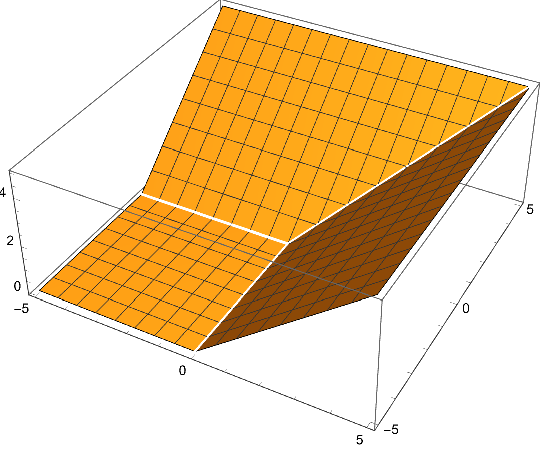
\includegraphics[width=0.3\textwidth]{figs/fig2-1-LinearTropicalPolynomial.pdf}}\quad
        \subcaptionbox{Projection onto $xy$-plane\label{fig:2.2-ProjectionLinearTropicalPolynomial}}{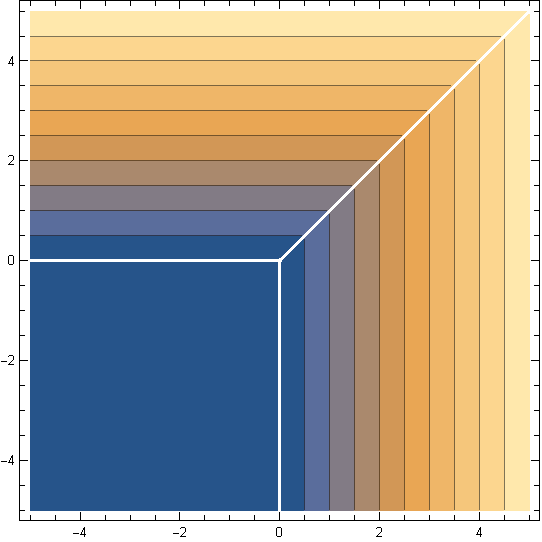
\includegraphics[width=0.25\textwidth]{figs/fig2-2-LinearTropicalPolynomialProjected.pdf}}\quad
        \subcaptionbox{Corner locus\label{fig:2.3-CornerLocus}}{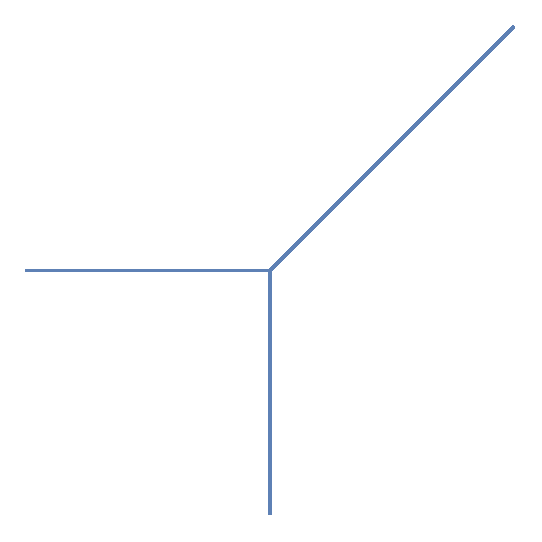
\includegraphics[width=0.25\textwidth]{figs/fig2-3-CornerLocus.pdf}}
        %\caption{This is the caption.}
        \label{fig:2.1-and-2.2-and-2.3}
    \end{figure}
    %https://mathematica.stackexchange.com/questions/169777/listplot3d-with-contours-projected-onto-the-xy-plane
    Observe that the surface is not smooth where the planes meet: We will call this the \emph{corner locus} or \emph{tropical hypersurface}.
    %In two variables we have a PICTURE. The polynomial $x\oplus y\oplus 0$ is actually $\max(x,y,0)$. This picture is actually the projection of the corner locus. In 3D we can visualize this better.
\end{Ex}

\begin{Def}
    The \term{tropical hypersurface}, $V(\Trop(p))$, is the codimension one locus in $\bR^n$ where the function is non-linear, also called the corner locus.
\end{Def}

\begin{Ex}
If we consider higher degree tropical polynomials, they will become linear in the usual sense. Consider 
$$p(x)=3x^2=3\odot x\odot x=3+x+x=3+2x,$$
which is indeed linear with respect to our usual definition of sum and product.
\end{Ex}

\subsection{Valued fields}

\begin{Def}
The field of \term{Puiseux series} or rational functions over $\bC$ is $\bC(t)$ where the elements are of the form 
$$f(t)=\sum_{i=k_0}^\infty a_it^{i/n}.$$
The lower bound, $k_0$, can be negative, and the exponents are rational numbers with bounded denominators. 
\end{Def}

Let us consider a quick example of a Puiseaux series to familiarize ourselves with them. 

\begin{Ex}
    Consider the Puiseux series 
    $$f(t)=\sum_{i=-12}^\infty -\frac{i}{12}t^{i/6}.$$
    If we expand out the first few terms, we get 
    $$\frac{12}{12}t^{-12/6}+\frac{11}{12}t^{-11/6}+\frac{10}{12}t^{-10/6}+\frac{9}{12}t^{-9/6}+\ldots=t^{-2}+\frac{11}{12}t^{-11/6}+\frac{5}{6}t^{-5/3}+\frac{3}{4}t^{-3/2}+\ldots$$
\end{Ex}
This field can be equipped with a valuation
$$\val_0\:\text{ }\bC(t)\to\bR\cup\set{\infty},\text{   }\begin{cases}
    0\mapsto \infty\\
    f\mapsto\text{order of vanishing at }0.
\end{cases}$$
This order of vanishing is the value $\al$ such that $\frac{f}{t^\al}$ approaches a finite non-zero value. Formally, we can express this as 
$$\val_0(f)=\min\Set{\al\leq\infty\:\ \lim_{t\to0}\frac{f}{t^\al}\in\obonj{0,\infty}}.$$
The corresponding coefficient in the series expansion of $f$ for this value is called the \term{valuation coefficient}.

\begin{Ex}
    In our original example, we can see that if we divide $f$ by $t^{-2}$ (or similarly multiply by $t^2$), we get 
$$t^2f(t) = 1 + \frac{11}{12}t^{1/6} + \frac{5}{6}t^{1/3} + \frac{3}{4}t^{1/2} + \ldots \xrightarrow[t\to0]{} 1 + 0 + 0 + \ldots$$
If we were to instead divide by a lower power of $t$, say $t^{-3}$, we would get 
$$t^3f(t) = t + \frac{11}{12}t^{7/6} + \frac{5}{6}t^{4/3} + \frac{3}{4}t^{3/2} + \ldots \xrightarrow[t\to0]{} 0 + 0 + \ldots$$
Even if zero is a finite value, we have stated that the order of vanishing makes $\frac{f}{t^\alpha}$ approach a finite \textbf{non-zero} value.\par 
On the other hand, if we were to divide by a higher power than $-2$, say $t^{-1}$, we get 
$$tf(t) = t^{-1} + \frac{11}{12}t^{-5/6} + \frac{5}{6}t^{-2/3} + \frac{3}{4}t^{-1/2} + \ldots \xrightarrow[t\to0]{} \infty.$$
So, in this case, we get a \textbf{non-finite} value. This example hopefully gives us the intuition that the order of vanishing is a unique value.

\end{Ex}

Some more questions now naturally arise: 
\begin{enumerate}
    \item What happens to the order of vanishing when we add two functions?
    \item What happens to the order of vanishing when we multiply two functions? 
\end{enumerate}

We consider an example to start. 

\begin{Ex}
    Consider two small functions, $f(t)=t^2$ and $g(t)=t^3$. Note that $\val_0(f) = 2$ and $\val_0(g) = 3$. 
    Additionally, $f+g=t^2+t^3$, so $\val_0(f+g) = 3.$ Observe that $2=\min(2,3)$.
\end{Ex}


In general. we get that
$$\val_0(f+g)\geq\min(\val_0 f,\val_0 g),\word{and}\val_0(fg)=\val_0(f)+\val_0(g).$$

We can do algebraic geometry over this field! Let $\bK$ be the field of Puiseux series. If $p(x_1,\dots,x_n)\in \bK\bonj{x_1,\dots,x_n}$, then we consider the algebraic variety
$$X=V(p)=\set{\vec{x}\in\bK^n\:p(\vec{x})=0}\subseteq \bK^n.$$
Each entry of $X$ is a Puiseux series of which we can take the valuation. The image through the $n$-fold valuation of $X$ will be a set in $\left(\bR\cup\set{\infty}\right)^n$. We will call the tropicalization of $X$ the image through this map. This is the tropical hypersurface for $p$.


\begin{figure}[h!]
    
\centering
\tikzset{every picture/.style={line width=0.75pt}} %set default line width to 0.75pt        

\begin{tikzpicture}[x=0.75pt,y=0.75pt,yscale=-1,xscale=1]
%uncomment if require: \path (0,300); %set diagram left start at 0, and has height of 300

%Straight Lines [id:da2454102694181276] 
\draw    (235,63) -- (299,63) ;
\draw [shift={(301,63)}, rotate = 180] [color={rgb, 255:red, 0; green, 0; blue, 0 }  ][line width=0.75]    (10.93,-3.29) .. controls (6.95,-1.4) and (3.31,-0.3) .. (0,0) .. controls (3.31,0.3) and (6.95,1.4) .. (10.93,3.29)   ;
%Straight Lines [id:da5779705315012776] 
\draw    (241,113) -- (298,113) ;
\draw [shift={(300,113)}, rotate = 180] [color={rgb, 255:red, 0; green, 0; blue, 0 }  ][line width=0.75]    (10.93,-3.29) .. controls (6.95,-1.4) and (3.31,-0.3) .. (0,0) .. controls (3.31,0.3) and (6.95,1.4) .. (10.93,3.29)   ;
\draw [shift={(241,113)}, rotate = 180] [color={rgb, 255:red, 0; green, 0; blue, 0 }  ][line width=0.75]    (0,5.59) -- (0,-5.59)   ;

% Text Node
\draw (208,53.4) node [anchor=north west][inner sep=0.75pt]    {$\bK^{n}$};
% Text Node
\draw (303,53.4) node [anchor=north west][inner sep=0.75pt]    {$(\bR\cup\set{\infty})^{n}$};
% Text Node
\draw (202,103.4) node [anchor=north west][inner sep=0.75pt]    {$V( p)$};
% Text Node
\draw (304,99.4) node [anchor=north west][inner sep=0.75pt]    {$\overline{\operatorname{val}_0( V( p))}$};
% Text Node
\draw (172,153.4) node [anchor=north west][inner sep=0.75pt]    {$\{\vec{x} :p(\vec{x}) =0\}$};
% Text Node
\draw (302,153.4) node [anchor=north west][inner sep=0.75pt]    {$\operatorname{Trop}( V( p))$};
% Text Node
\draw (210.4,98) node [anchor=north west][inner sep=0.75pt]  [rotate=-270]  {$\subseteq $};
% Text Node
\draw (328.4,98) node [anchor=north west][inner sep=0.75pt]  [rotate=-270]  {$\subseteq $};
% Text Node
\draw (229.6,127) node [anchor=north west][inner sep=0.75pt]  [rotate=-90]  {$=$};
% Text Node
\draw (346.6,127) node [anchor=north west][inner sep=0.75pt]  [rotate=-90]  {$=$};
% Text Node
\draw (172,53.4) node [anchor=north west][inner sep=0.75pt]    {$\operatorname{val}_0\:$};


\end{tikzpicture}
\caption{Diagram on the tropical hypersurface}
\label{fig:2a-diagram-trop-hypersurf}
\end{figure}


\begin{Ex}
    Consider the polynomial in $\bK\bonj{x,y}$,
    $$p(x,y)=tx+y+t^2.$$
    The variety is $X=\set{(x,y)\: tx+y+t^2=0}=\{ (x,y) \; |\; y = -tx -t^2\}$. We can solve the equation $y=-tx-t^2$.\par 
    If we choose $x=0$, then $y$ becomes $-t^2$. Now we take the valuation of $(0,-t^2)$, and so $(\infty,2)$ is a point in $\Trop(X)$.
\end{Ex}

\section{Intro}



\begin{ex}
    We consider the case where our input can be a line in the plane $\CC^2$, i.e. $az+bw=d$. Then the output of the construction can be a tripod/tropical $Y$, i.e. three lines connecting a vertex.


    Our input could also be an elliptic curve in $\CC^2$, and thus the output could be another, more complicated connection of verticles and lines (a tropical cubic). 


    Lastly, we can consider an abstract nodal curve (a sphere and tori connected at verticies), with the corresponding piecewise lienar object being a dual graph, which has a vertex at each component, an edge for each node, and a label for each part.
\end{ex}


\subsection{Amoebas}


Let us return to the usual stage and consider $p\in\bC[x_1,\dots,x_n]$, which defines an algebraic variety $X=V(p)\subseteq\bC^n$. We can consider the map which sends every coordinate's modulus to its logarithm in base $t$: 
$$\bC^n\to\left(\bR\cup\set{-\infty}\right)^n,\quad (z_1,\dots,z_n)\to(\log_t|z_1|,\dots,\log_t|z_n|).$$


The image of $X$ under this map, $\log_t(X)$, is the $t$-amoeba of $X$. If we take the limit as $t\to\infty$, then we get the \emph{spine} of the amoeba. 



\begin{Ex}
    When $p(x,y)=x+y-1$, then we can describe $V(p)$ via the parametrization $(x,1-x)$. So the corresponding $t$-amoeba in the real case is 
    $$\set{(\log_t|x|,\log_t|1-x|)\: x\in\bR}.$$
    If we take the limit in the ordinary sense,$\lim_{t\to\infty}\frac{\log|x|}{\log t}$, we see that the functions converge to zero point-by-point. But the set as a whole is actually approaching the spine!
    \begin{figure}[h!]
        \centering
        \subcaptionbox{$X=V(x+y-1)$\label{fig:2.4-Variety}}{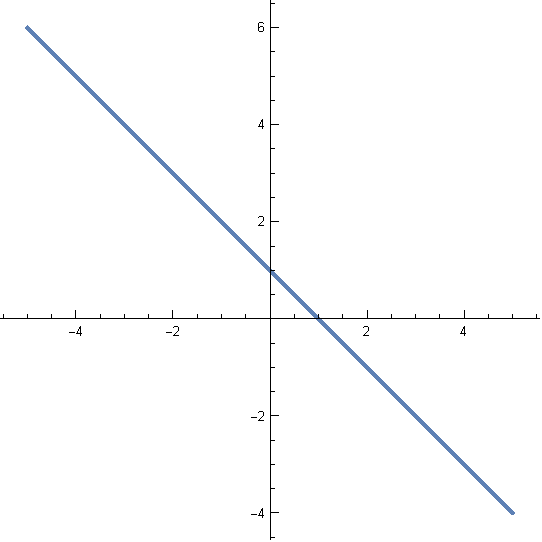
\includegraphics[width=0.25\textwidth]{figs/fig2-4-V(x+y-1).pdf}}\quad
        \subcaptionbox{$2$-amoeba of $X$\label{fig:2.5-2Amoeba}}{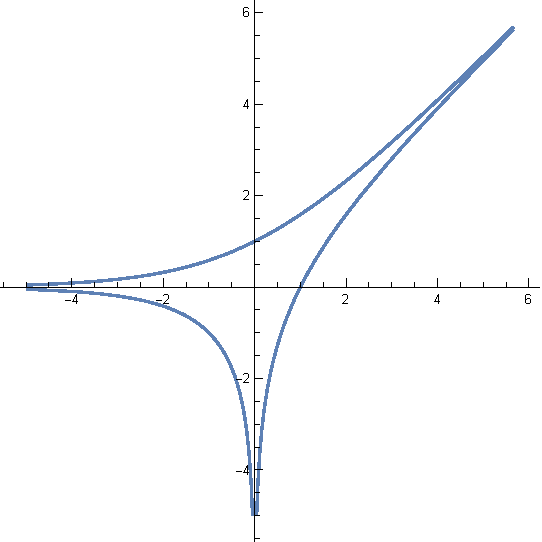
\includegraphics[width=0.25\textwidth]{figs/fig2-5-2amoeba.pdf}}\quad
        \subcaptionbox{Sequence of amoebas as $t\to\infty$\label{fig:2.6-ApproxAmoebas}}{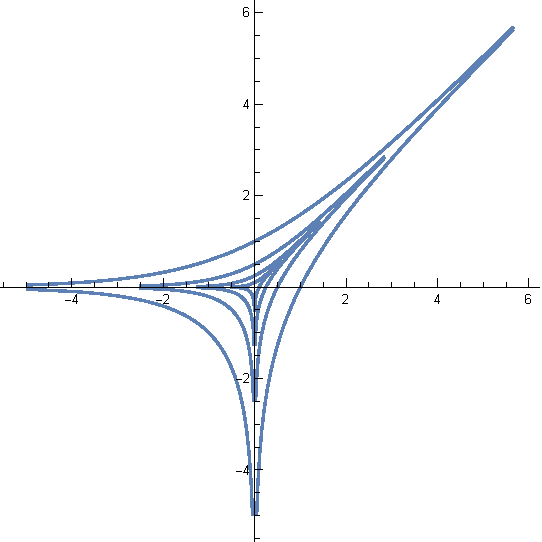
\includegraphics[width=0.25\textwidth]{figs/fig2-6-ApproximatingAmoebas.pdf}}
        %\caption{This is the caption.}
        \label{fig:2.4-thru-2.6}
    \end{figure}
\end{Ex}

Observe that the spine approaches the tropical hypersurface associated to $p$. In other words, we have that the tropical hypersurface is $\lim_{t\to\infty}\log_t(V(p))$.


\subsection{Degenerations of Algebraic Varieties}
We may parametrize any algebraic variety with a time variable. Then in converting the information to a graph, the edges encode the information about how fast the node forms related to the length.\par
Consider a family of \red{of what, what is this family of?! Stuff? Curve in P1xP1 which eventually becomes P2?}
\begin{figure}[h!]
    \centering
    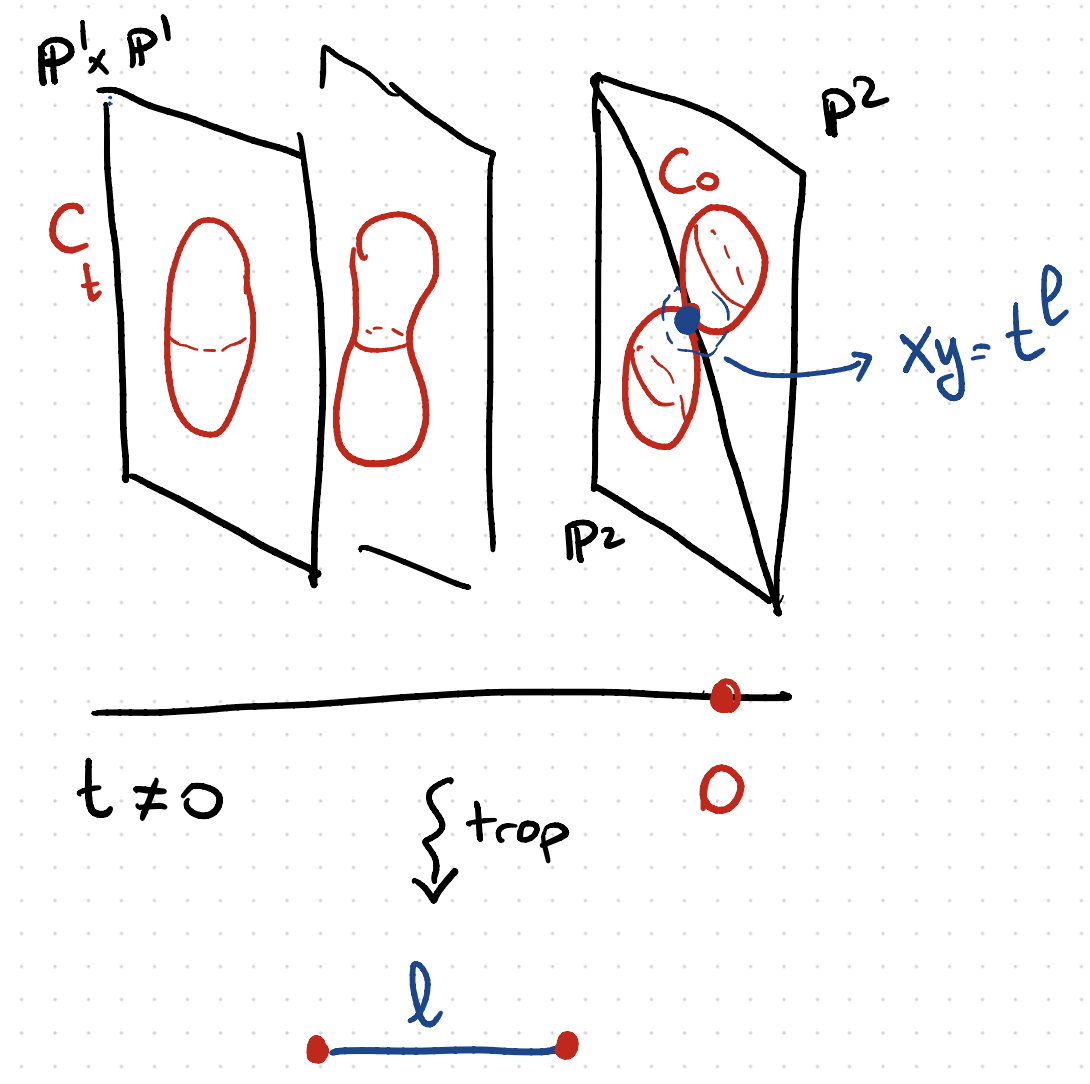
\includegraphics[width=0.5\textwidth]{figs/fig1-1.png}
\end{figure}

It is too early to understand this rather complicated point of view. We will set everything up to get to it.\par 
In general, the big idea will be to explore and understand these perspectives in the case of plane curves. We want to show how they are equivalent and then recover classical algebraic geometry results in terms of tropical geometry.

\subsection{Tropical Arithmetic}%%%Based on TropicalNumbers.pdf

We now would like to answer the question
\begin{significant}
    Where do tropical numbers come from?
\end{significant}
Let us begin with an application problem and see how the tropical numbers arise from its context.

\subsubsection{Minimizing Tolls}

Consider a set of cities connected by a network of toll-ways:
\begin{figure}[h!]
    \centering
    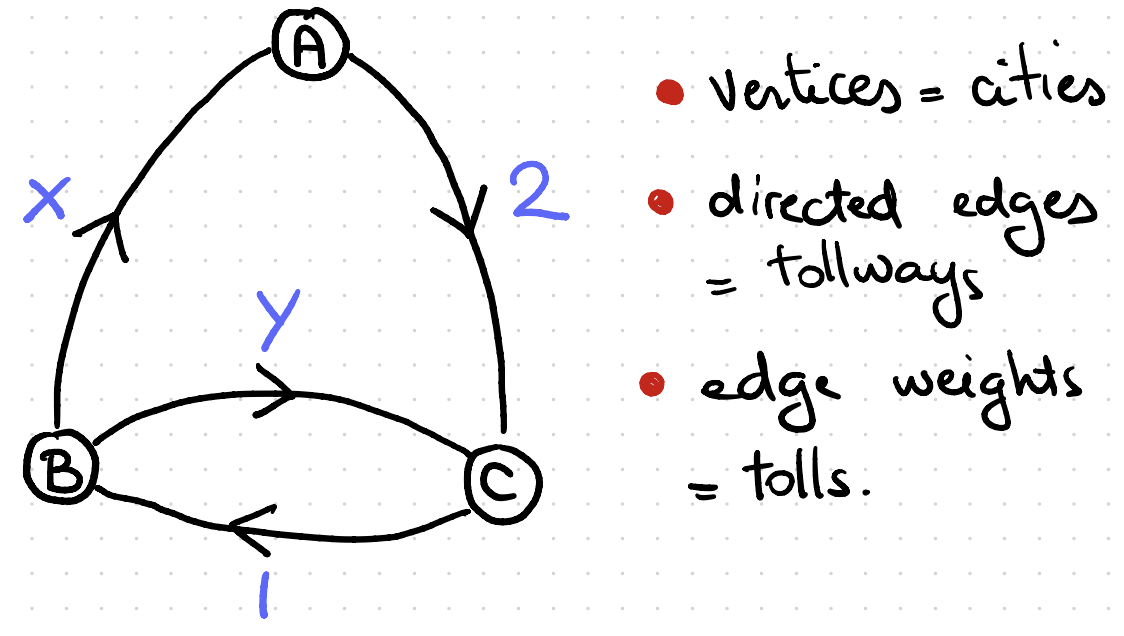
\includegraphics[width=0.5\textwidth]{figs/fig1-2.png}
\end{figure}

If we only care about minimizing toll expenses when traveling, what would be the cheapest way to go from one given city to another? Let us record the information as an incidence matrix:
$$M_{ij}=\text{price of going from city }i\text{ to city }j\text{ in at most one trip}\To M=\threebythree{0}{\infty}{2}{x}{0}{y}{\infty}{1}{0}$$

In this matrix, the rows determine the outbound city, while the columns are the destination. Each entry records the cost of a toll and tolls are considered to be infinite when the road does not exist. So, for example, there is a toll road from A to C which costs two dollars, but there is no road from A to B. We can also think of $M$ as recording the cheapest toll to go from one city to another with at most one move.\par 
How would we compute the best strategy of going from city $i$ to $j$ in \emph{at most two trips}? If, for example, we want to find trips from $A$ to $B$ in two steps, then we have three choices:
$$AAB,\quad ABB,\quad ACB.$$
The costs of each one respectively are 
$$(0,\infty),\quad (\infty,0),\quad (2,1)$$
To find the optimal route, we sum these costs and take the minimum. In fact, if we relate this to the entries of the matrix $M$, we could use $M^2$. However, we must redefine our basic operations as follows: 
$$+=\min,\quad\.=+$$
So we have the identification 
$$(1,2)\text{ entry of }M^2=\sum_{j=1}^{3}M_{1k}M_{k2}=\min(M_{11}+M_{12},M_{12}+M_{22},M_{13}+M_{32}).$$
In general:
\begin{align*}
    \threebythree{0}{\infty}{2}{x}{0}{y}{\infty}{1}{0}^2&=\threebythree{\min\threebyone{0+0}{\infty+x}{2+\infty}}{\min\threebyone{0+\infty}{\infty+0}{2+1}}{\min\threebyone{0+2}{\infty+y}{2+0}}{\min\threebyone{x+0}{0+x}{y+\infty}}{\min\threebyone{x+\infty}{0+0}{y+1}}{\min\threebyone{x+2}{0+y}{y+0}}{\min\threebyone{\infty+0}{1+x}{0+\infty}}{\min\threebyone{\infty+\infty}{1+0}{0+1}}{\min\threebyone{\infty+2}{1+y}{0+0}}\\
    &=\threebythree{0}{3}{2}{x}{\min(0,y+1)}{\min(x+2,y)}{1+x}{1}{\min(0,1+y)}.
\end{align*}
Observe that $1+y$ can be the minimum in the diagonal when we allow \emph{negative tolls}.

\begin{Rmk}
If we disallow negative tolls, the products $M^n$ eventually stabilize to a matrix whose entries record the cheapest way to get from one city to another in $n$ steps.
\end{Rmk}
This gives us the intuition that minimization problems eventually correspond to linear algebra problems over $(\bT,+,\.)$ which is precisely $(\bR\cup\set{\infty},\min,+)$.

\subsubsection{Forgetting phases}



Another context we can consider is related to physics/electromagnetism. If we take a complex number, we can write it in polar coordinates, i.e. $z \in \CC$ can be written as $z = rho e^{i \theta}$. Suppose we do not particularly care about the phase ($\theta$), or that we are working on a logarithmic scale. Then we consider the function would be $T_t\:\bC\to\set{-\infty}\cup\bR,\quad z\mapsto\log_t(|z|)$. We add the point at negative infinity in order to define $T_t(0)$.

\begin{figure}[h!]
    \centering
    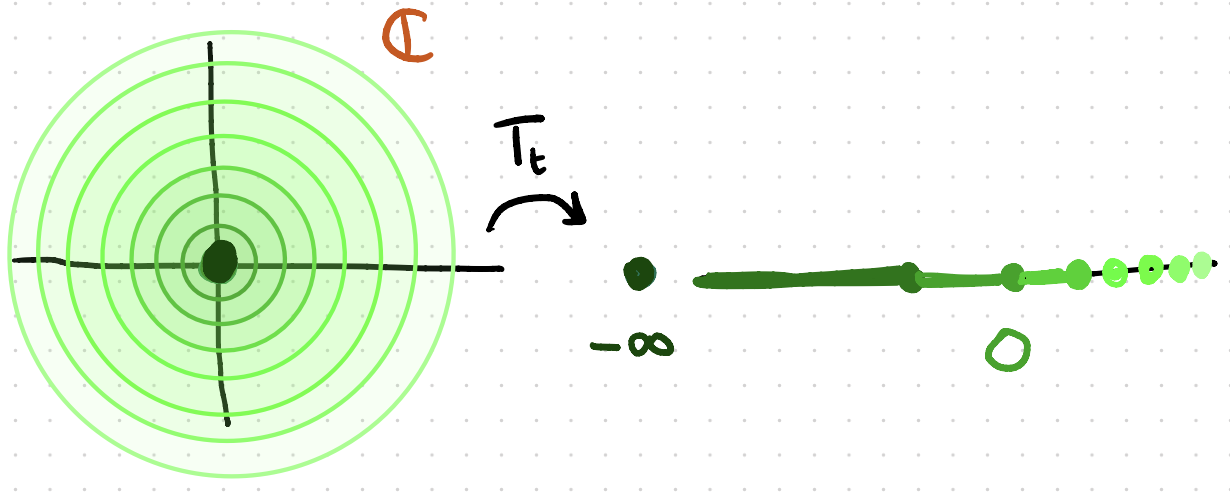
\includegraphics[width=0.5\textwidth]{figs/fig1-3.png}
\end{figure}


Note that this map is surjective. Any $x\in\bR$ is 
$$T_t(t^xe^{i\te})=\log_t|t^xe^{i\te}|=\log_tt^x=x,\quad\te\in\bR.$$
This means that the inverse image of a point contains a plethora of points, in fact:
$$
\left\lbrace
\begin{aligned}
    &T_t^{-1}(x)=\set{t^xe^{i\te}}\subseteq\bC,\word{for}x\in\bR,\\
    &T_t^{-1}(-\infty)=0.
\end{aligned}
\right.
$$
With this in mind, we wish to define an exotic addition and multiplication on $\set{-\infty}\cup\bR$ using $T_t$. We will dequantize!\par 


We begin with \textbf{hyper-addition}. The output will be a subset of $\set{-\infty}\cup\bR$ so notice that this is not a binary operation by itself. 
$$x\diamondplus_t y\:= T_t(T_t^{-1}(x)+T_t^{-1}(y))=\bonj{\log_t(|t^x-t^y|),\log_t(t^x+t^y)}.\label{problem1-hyperAddition}$$
This is an interval in $\set{-\infty}\cup\bR$. In order to make $\diamondplus_t$ into a true operation, we take a limit:
\begin{figure}[h!] 
    \centering
\begin{tikzpicture}[x=0.75pt,y=0.75pt,yscale=-1,xscale=1]
%uncomment if require: \path (0,300); %set diagram left start at 0, and has height of 300

%Straight Lines [id:da5156276968518897] 
\draw    (85,62.6) -- (142,62.99) ;
\draw [shift={(144,63)}, rotate = 180.39] [color={rgb, 255:red, 0; green, 0; blue, 0 }  ][line width=0.75]    (10.93,-3.29) .. controls (6.95,-1.4) and (3.31,-0.3) .. (0,0) .. controls (3.31,0.3) and (6.95,1.4) .. (10.93,3.29)   ;

%Straight Lines [id:da8224691621679702] 
\draw    (96,133) -- (144,133.38) ;
\draw [shift={(146,133.4)}, rotate = 180.46] [color={rgb, 255:red, 0; green, 0; blue, 0 }  ][line width=0.75]    (10.93,-3.29) .. controls (6.95,-1.4) and (3.31,-0.3) .. (0,0) .. controls (3.31,0.3) and (6.95,1.4) .. (10.93,3.29)   ;
%Straight Lines [id:da27001319663870027] 
\draw    (57,77) -- (57,118) ;
\draw [shift={(57,120)}, rotate = 270] [color={rgb, 255:red, 0; green, 0; blue, 0 }  ][line width=0.75]    (10.93,-3.29) .. controls (6.95,-1.4) and (3.31,-0.3) .. (0,0) .. controls (3.31,0.3) and (6.95,1.4) .. (10.93,3.29)   ;
%Straight Lines [id:da8909494911629017] 
\draw    (195,83) -- (195,120) ;
\draw [shift={(195,122)}, rotate = 270] [color={rgb, 255:red, 0; green, 0; blue, 0 }  ][line width=0.75]    (10.93,-3.29) .. controls (6.95,-1.4) and (3.31,-0.3) .. (0,0) .. controls (3.31,0.3) and (6.95,1.4) .. (10.93,3.29)   ;

% Text Node
\draw (34,53.4) node [anchor=north west][inner sep=0.75pt]    {$x\diamondplus_t y$};
% Text Node
\draw (34,123.4) node [anchor=north west][inner sep=0.75pt]    {$x\ +_{t} \ y$};
% Text Node
\draw (152,53.4) node [anchor=north west][inner sep=0.75pt]    {$x\diamondplus y=\lim _{t\rightarrow \infty } x\diamondplus_t y$};
% Text Node
\draw (152,123.4) node [anchor=north west][inner sep=0.75pt]    {$x+y=\max( x,y)$};
% Text Node
\draw (60,98.5) node [anchor=west] [inner sep=0.75pt]  [font=\scriptsize]  {$\max$};
% Text Node
\draw (114.5,59.4) node [anchor=south] [inner sep=0.75pt]  [font=\scriptsize]  {$\displaystyle\lim _{t\rightarrow \infty }$};
% Text Node
\draw (121,129.8) node [anchor=south] [inner sep=0.75pt]  [font=\scriptsize]  {$\displaystyle\lim _{t\rightarrow \infty }$};
% Text Node
\draw (197,102.5) node [anchor=west] [inner sep=0.75pt]  [font=\scriptsize]  {$\max$};


\end{tikzpicture}

\end{figure}



\begin{Rmk}
Note that $\diamondplus$ is still a hyperoperation. Its output is not a singleton \emph{only} when adding a number to itself:
$$x\diamondplus y=\begin{cases}
    \max(x,y),\quad x\neq y\\
    \bonj{-\infty,x},\quad x=y
\end{cases}$$
\end{Rmk}

Formally this process, taking a limit of a family of operations, is known as \emph{dequantization}.\par

In the case of multiplication, the definition is much more straightforward:

$$x\.y =T_t\bonj{T^{-1}(x)\.T^{-1}(y)}=\log_t\bonj{|(t^xe^{i\te})(t^ye^{i\vf})|}=\log_tt^{x+y}=x+y$$


Why is this better? Let us consider a small example. 

\begin{Ex}
    Observe that 
    $$4\diamondplus_t 2=T_t(T_t^{-1}(4)+T_t^{-1}(2))=T_t\left|t^4e^{i\te}+t^2e^{i\vf}\right|$$
    and the term on the inside can be simplified to $t^{4}(e^{i\te}+t^{-2}e^{i\vf})$. $T_t$ takes that expression to
    $$4+\log_t|e^{i\te}+t^{-2}e^{i\vf}|=4+\frac{\log|e^{i\te}+t^{-2}e^{i\vf}|}{\log t}.$$
    What happens if we take the limit as $t\to\infty$? We get a result that is independent from $t$! 
    The term on the right vanishes, and we are left with $4=\max(4,2)$. This is a tad bit better, but it is still a hyperoperation!
\end{Ex}

\begin{Ej}
Check how the definition of $+$ and $\.$ extend to the \emph{number} $-\infty$.
\end{Ej}

\begin{ptcb}
The point of this exercise is to operate $-\infty$ with both finite numbers and itself.\par
For a finite $x$, we will find $x+(-\infty)$. This is the limit of the previous hyperoperation:
$$x\diamondplus_t(-\infty)=T_t(T_t^{-1}(x)+T_t^{-1}(-\infty))=T_t(T_t^{-1}(x)+0)=T_t(T_t^{-1}(x))=x.$$
If we let $t$ grow, the result does not change, and so this behaves in accordance with $\max(x,-\infty)=x$.\par 
On the other hand, when taking the product:
$$x\.(-\infty)=T_t\bonj{T^{-1}(x)\.T^{-1}(-\infty)}=T_t\bonj{T^{-1}(x)\.0}=T_t(0)=\log_t(0)\to-\infty,$$
which is also similar to the notion of $x+(-\infty)=-\infty$.\par 
We can now operate $-\infty$ with itself:
$$(-\infty)\diamondplus_t(-\infty)=T_t(0)=\log_t(0)=-\infty=\max(-\infty,-\infty),$$
and when taking the product:
$$(-\infty)\.(-\infty)=T_t(0)\log_t(0)=-\infty=(-\infty)+(-\infty),$$
where the last sum is a sum in the usual sense.
\end{ptcb}

So, summarizing this process:
\begin{itemize}
    \item We forgot about the phase of the complex numbers and only looked at them radially. 
    \item The modulus of these numbers was scaled logarithmically.
    \item Finally, we took the limit of these operations and obtained the desired (somewhat) result.
\end{itemize}
This is known as Maslov\footnote{Viktor Pavlovich Maslov (1930615-20230803)} dequantization. With this, we can see $(\bT,+,\.)$ as $(\set{-\infty}\cup\bR,\max,+)$. Note, we will abbreviate $\lim_{t\to\infty}T_t$ with $T_{t\to\infty}$

\section{Interim 1|Valuations}
%%valued fields and puiseux seires

\subsection{Valuations}

In essence, a valuation provides a measure of the \emph{size} (or multiplicity) of elements in a field. 

\begin{Def}
    If $K$ is a field, a \term{valuation} on $K$ is a mapping
    $$\val\:\ K\to\bR\cup\set{\infty}$$
    with the properties:
    \begin{enumerate}[i)]
        \itemsep=-0.4em 
        \item $\val(x)=\infty\iff x=0$,
        \item $\val(xy)=\val(x)+\val(y)$,
        \item $\val(x+y)\geq\min(\val(x),\val(y))$, with equality if $\val(x)\neq\val(y)$.
    \end{enumerate}
    In this case, we say that $K$ is a valued field.
\end{Def}

Previous discussion has shown us that the order of vanishing, $\val_0$, is a valuation of the field of Puiseux series $\bK$. The above properties can be shown to be true for $K$ by writing out two Puiseux series and checking them directly.

\begin{Ej}
Verify that the field of Puiseux series is indeed a valued field with valuation $\val_0$.
\end{Ej}

There is also a another common example, the $p$-adic valuation, which comes from number theory.\par
We first define the valuation on $\bZ$ as 
$$v_p(a)=\max\set{k\in\bZ\:\ p^k\mid a},$$
 where $p$ is a prime number. For the rational numbers, the valuation is defined as $v_p(m/n)=v_p(m)-v_p(n)$.\par
This valuation can be used to study the field of $p$-adic numbers, which is the completion of $\bQ$ with respect to the $p$-adic absolute value $|r|_p=p^{-v_p(r)}$.

\begin{Ej}
In a similar fashion, verify that $v_p$ is a valuation over $\bQ$.
\end{Ej}

\chapter{The Tropical Numbers}

\section{Day 4|20230828}

We have now seen where our ideas and intuition come from. Certain kinds of minimization problems give rise to our tropical numbers, and by expressing complex numbers in a logarithmic scale without phase, inducing a sum actually gives us a hypersum. The was converted into an operation by taking a limit, and the algebraic structure we obtained was once again the tropical numbers. Let us talk more formally about the perspective of valued fields.

\subsection{Puiseux series}
Recall from our time in Calculus class that when resolving indeterminate limits, the relevant information is contained in the order of vanishing of the function.

\begin{Ex}
    Consider the limit $\lim_{t\to 0}\frac{\sin(x)}{x}=1$. Near $t=0$, we have 
    $$\sin(t)=t+o(t)\sim t^1\word{and}\frac{1}{t}=t^{-1},\word{so}t^1t^{-1}=t^0=1.$$
\end{Ex}

From this, we wish to study the orders of zeroes and poles of Laurent series. In order to extend the class of functions to an algebraically closed field, we consider Puiseux series, or rational functions. We can identify Puiseux series as 
$$\bC\set{\set{t}}=\bigcup_{n\in\bN}\bC(t^{1/n}).$$
Concretely, elements here are Laurent series with rational exponents, and the exponents of terms with non-zero coefficients have a common denominator. 
\begin{Ex}
    The series $\sum_{k=-37}^{\infty}t^{k/42}$ is a Puiseux series. However $\sum_{k=1}^\infty t^{1/k}$ is \emph{not} a Puiseux series.
\end{Ex}
This is the most natural algebraically closed field with a \emph{canonical} valuation. This is the function:
$$\val: \bC\set{\set{t}}\to\bR\cup\set{\infty},\begin{cases}
    0\mapsto\infty\\
    t^{p/q}+\text{higher order}\mapsto p/q
\end{cases}$$

In other words, the valuation sends $\sum_{k=k_0}^\infty a_kt^{q_k}$ to $q_{k_0}$.

\begin{Prop}\label{prop:PropertiesOfValuation}
For $\al,\bt\in\bC\set{\set{t}}$, the valuation satisfies the following properties:
\begin{enumerate}[i.]
    \item $\val(\al\.\bt)=\val(\al)+\val(\bt)$.
    \item $\val(\al+\bt)\geq\min(\val(\al),\val(\bt))$.
\end{enumerate}
Equality holds when $\val(\al)\neq\val(\bt)$.
\end{Prop}

So, if we decide to define operations on $\bR\cup\set{\infty}$ by inducing them from the operations on $\bC\set{\set{t}}$, we obtain the hyperoperation
\begin{align*}
    &x\diamondplus y=\val\left(\val^{-1}(x)+\val^{-1}(y)\right),
    &x\. y=\val\left(\val^{-1}(x)\.\val^{-1}(y)\right).
\end{align*}
Now $\.$ coincides with usual addition, and $+$ is the hyperoperation
$$x\diamondplus y=\begin{cases}
    \min(x,y)\word{when}x\neq y,\\
    [\min(x,y),\infty]\word{when}x=y.
\end{cases}$$
\begin{Ex}
    If we attempt to sum $0$ with itself, we get 
    $$0\diamondplus 0=\val\left((a_0+a_1t^{q_1}+\dots)+(-a_0+b_1t^{r_1}+\dots)\right).$$
    Note that this could be either $q_1$ or $r_1$ because the constant terms cancel! 
\end{Ex}
The only natural way to turn this into an operation is to define $x+y=\min(x,y)$. In conclusion, the field of Puiseux series with the order of vanishing and poles is congruent to $(\bT,+,\.)$, which in this case is $\left(\bR\cup\set{\infty},\min,+\right)$.

\subsection{The Tropical Semifield}

\begin{Def}
    The \term{tropical semifield} is $(\bT,\oplus,\odot)$ where we can choose either:
    \begin{itemize}
        \item $\bT=\bR\cup\infty$, $\oplus$ to be $\min$ and $\odot$ is $+$ (called the min convention)
        \item $\bT=\set{-\infty}\cup\bR$, $\oplus=\max$ and $\odot=+$ (called the max convention).
    \end{itemize}
\end{Def}

There is a natural isomorphism between the two choices given by $x\mapsto -x$. As we have mentioned, different contexts may be more natural than the other when using certain conventions. For our purposes, we will typically utilize the $\max$ convention. 

\begin{Prop}
The following algebraic properties hold for $(\bT,+,\.)$:
\begin{enumerate}[i)]
    \itemsep=-0.4em
    \item $0_\bT=-\infty$.
    \item $1_{\bT}=0$.
    \item The only solution of $x\oplus y=0_\bT$ is $x=y=0_\bT$. This means that only $-\infty$ has an additive inverse.
    \item Addition is idempotent, i.e. $x\oplus x=x$.
    \item Every non-zero element has a multiplicative inverse such that $1/x=-x$.
\end{enumerate}
\end{Prop}

\begin{ptcbp}
    \begin{enumerate}[i)]
        \itemsep=-0.4em
    \item Observe that $x\oplus0_\bT=\max(x,-\infty)=x$.
    \item $x\odot 1_\bT=x+0=x$.
    \item $x\oplus y=0_\bT\iff \max(x,y)=-\infty\To x=y=-\infty$.
    \item $x\oplus x=\max(x,x)=x$.
    \item $x\.(1/x)=x+(-x)=0=1_\bT$.
\end{enumerate}
\end{ptcbp}
Observe that it is not possible to adjoin formal additive inverses. Suppose that for $x\in\bT$, there exists a $y$ such that $x+y=0_\bT$. Then 
$$(x\oplus x)\oplus y=x\oplus y=0_\bT\word{and}x\oplus (x\oplus y)=x\oplus 0_\bT=x,\word{but}x\neq 0_\bT.$$
This means that any invertible element necessarily has to be $-\infty$.

\begin{Ej}
What other algebraic properties do these operations satisfy? We have claimed, for example, that $\oplus$ is associative. Prove this.\par 
Are the operations commutative? Do they distribute with respect to each other?
\end{Ej}

\begin{ptcb}
Let us assume without loss of generality that 
$$x<y<z.$$
Then 
\begin{align*}
    &x\oplus (y\oplus z)=\max(x,\max(y,z))=\max(x,z)=z\\
    &(x\oplus y)\oplus z=\max(\max(x,y),z)=\max(y,z)=z,
\end{align*}
which shows us that $\oplus$ is associative. We can see that it is commutative by realizing that $\max$ is also commutative.\par 
Finally, we wish to know if distribution holds. First observe that 
$$y<z\To x+y<x+z.$$
We can see that 
\begin{align*}
&x\odot(y\oplus z)=x\odot y\oplus x\odot z\\
\iff &x+\max(y,z)=\max(x+y,x+z)\\
\iff &x+z=x+z,
\end{align*}
which proves that distribution does indeed hold. Note that it is not necessary to check distribution on the other side as our operations are commutative.
\end{ptcb}

\begin{Prop}[Weird Fun Facts]
Recall that the usual Pascal's Triangle is built by adding the previous two elements to get the next one. In the tropical case, we have all 0's:
$$
%https://tex.stackexchange.com/questions/17522/pascals-triangle-in-tikz
\begin{tikzpicture}
    \foreach \n in {0,...,2} {
      \foreach \k in {0,...,\n} {
        \node at (\k-\n/2,-\n) {$1_\bT$};
      }
    }
    \end{tikzpicture}
    \word{\raisebox{2.5em}{=}}%tex.se/47016
    \begin{tikzpicture}
        \foreach \n in {0,...,2} {
          \foreach \k in {0,...,\n} {
            \node at (\k-\n/2,-\n) {$0$};
          }
        }
        \end{tikzpicture}
    $$
    and this extends downwards with the same pattern.\par 
    We also get  a "freshman's dream" type of identity:
    $$(x\oplus y)^n=x^n\oplus y^n.$$

In other words, the tropical version of the binomial theorem is just a restatement of the identity $n\max(x,y)=\max(nx,ny)$.
\end{Prop}

\begin{Ej}
Recall that the coefficients in the expansion for the binomial theorem are the corresponding elements in the rows of Pascal's Triangle. Verify that the coefficients agree in the tropical case for the binomial theorem.
\end{Ej}

\begin{ptcb}
We must verify that the coefficient of every monomial in the expansion of $(x\oplus y)^n$ does match the $n^{\text{th}}$ row of Pascal's triangle. To that effect, note that 
\begin{align*}
    (x\oplus y)^n&=(x\oplus y)\odot(x\oplus y)\odot\dots\odot(x\oplus y)\\
    &=x^n\oplus x^{n-1}y\oplus\dots\oplus xy^{n-1}+y^n\\
    &=x^n\oplus y^n.
\end{align*}
In the second line, recall that we would usually have $\binom{n}{k}$ terms of the form $x^ky^{n-k}$. However, since addition is idempotent here, all those terms become just one single term.\par 
Also, observe that the coefficient (tropically) multiplying each term is $1_\bT$. This is because multiplication by 1 is simply adding 0. So it is indeed the case that all coefficients in the binomial expansion are $1_\bT$.\par 
Finally, observe that for any $k$, $kx+(n-k)y\leq\max(nx,ny),$ which means that the only terms that survive are the power $n$ monomials in the expansion. 
\end{ptcb}

Note that the fact taht $x^2 \oplus (x \odot ) \oplus y^2 = x^2 \oplus y^2$ does not imply cancellation, i.e. we do not automatically have that $x \odot y = -\infty$.


\subsubsection{The Optimal Assignment Problem}

Suppose we have $n$ jobs for $n$ workers. Each worker can only work one job, and once the job is taken, no one else can do it. We wish to assign a job to each worker in order to maximize our company's profit.

\begin{Ex}
    As a small example, consider Alice and Bob's hydroponics farm. When working with the weeds, Alice produces $5$ credits, and while working with the water, she produces $6$. On the other hand, Bob produces $3$ and $5$ respectively.\par 
    It is easy to see that Alice should be assigned to the weeds and Bob to the water in order to maximize. But let us apply what we know with tropical arithmetic.\par 
    Let 
    $$M_{ij}=\text{amount of credits work }i\text{ produces when doing job }j.$$
    Then we can summarize the previous information in a matrix 
    $$M=\twobytwo{5}{6}{3}{5},$$
    and if we take the tropical determinant, we get
    $$\Trop\det M=5\.5+6\.3=\max(5+5,6+3)=10,$$
    which is the maximal profit we can make by best assigning our workers to jobs.
\end{Ex}


In general, we define $tropdet(X) = \sum_{\sigma \in S_d}  \prod_{\sigma(i)}x$,where the sum is the tropical sum and the product is the tropical product. We do not get a signed determinant because tropical geometry does not have subtraction, so our tropical determinant is really a permanent.


\begin{Ej}
    Do the following:
    \begin{enumerate}[i)]
        \itemsep=-0.4em
        \item Construct a $3\x3$ matrix with non-permuted entries such that there is more than one possible assignment for the optimal jobs.
        \item Use the combinatorial definition of a permanent to show that the tropical determinant of $M$ is indeed the maximal profit. \hint{The definition of permanent is the same as the determinant but without the $(-1)^{\sgn\sg}$.}
        \item Assuming you know the tropical determinant of a matrix, devise a way to identify one job combination which reaches the optimum value. \aside{It is not actually necessary to know the value of the determinant!}
    \end{enumerate}
\end{Ej}

\begin{ptcb}
    \begin{enumerate}[i)]
        \itemsep=-0.4em
        \item Consider a matrix $A\in \bR^{3\x3}$. For a given $n\in\bN$, which will be our profit, we may build an infinite family of matrices which satisfy the required conditions.\par 
        The conditions our matrix must satisfy are sums of permuted entries.\par 
        In this case, the solution is given by $5$ parameters, including the profit:
        $$(n-f-h,n-g-g,n-f-g-h+i,f+g-i,f+h-i,f,g,h,i).$$
        An example of a valid matrix is 
        $$\threebythree{1}{3}{1}{3}{5}{3}{2}{4}{2}.$$
        \item The permanent by definition is 
        $$\bigoplus_{\sg\in S_n}\bigodot_{i=1}^n M_{i\sg_i}=\max_{\sg\in S_n}\left(\sum_{i=1}^n M_{i\sg_i}\right).$$
        The right hand side gives us the largest out of all the possible permutations, which is the highest sum over all possible job assignments, so the permanent will indeed find the maximal profit.
        \item We can proceed with a greedy algorithm. Row by row, choose the largest element, then eliminate the column the found element was in and repeat this process.\par 
        For example, pick $A_{1k}=\max(\text{row }1)$, then throw out column $k$ and repeat the process with the $(1,k)$ minor of $A$.\aside{This doesn't actually prove that the greedy algorithm works.} 
    \end{enumerate}
\end{ptcb}

\begin{Rmk}
Observe that the first problem can be solved in any dimension $d$ because in total, we have $2d$ equations while having $d^2$ indeterminates. Since $2d<d^2$ for $d\geq 2$, we have that the problem will always be under-determined. Thus, there is always more than one possible optimal assignment. 
\end{Rmk}

We now pose another question: 
\begin{significant}
    Is there an instance in which the greedy algorithm fails to find an optimal assignment for the jobs?
\end{significant}

\begin{Ej}
Prove or disprove that the greedy algorithm will find an optimal assignment for the jobs given the conditions above. You may assume to know the value of the permanent of the matrix.
\end{Ej}


\subsection{Tropical Polynomials and Roots}

A tropical univariate (Laurent) monomial is corresponds to an affine linear function with integer coefficients. Such a monomial is an expression of the form 
$$a\odot x^{\odot m},\quad a\in\bT,\quad m\in\bZ.$$

\begin{Ex}
    Consider
    $$5x^2\otto 5+2x\text{ and } 2x^{-3}\otto 2-3x.$$
    The second example is a Laurent monomial because of the negative power.\par
    Also consider $\sqrt 5\odot x^{\odot 3}$, which corresponds to $y=\sqrt{5}+3x$. Notice how the slope is always an integer, but the translation can be any number. This is an affine linear transformation because we can shift via $a,$ and it has integer slope $m.$ Furthermore, $$\{-\infty\}\odot x^{\odot m} = -\infty + mx = - \infty,$$ so we maintain that multiplying by the additive identity gives the additive identity.
\end{Ex}

A tropical univariate (Laurent) polynomial is a finite sum of monomials which give rise to a \emph{convex}, continuous, piecewise, affine linear function with integer slopes. 

\begin{Ex}
    Consider $p(x)=-5\odot x^{\odot2}\oplus(-2)\odot x^{\odot-3}\oplus 0,$ which corresponds to 
    $$\max(-5+2x,-2-3x,0).$$
    If we graph these functions, we obtain
    \begin{figure}[h!]
        \centering
        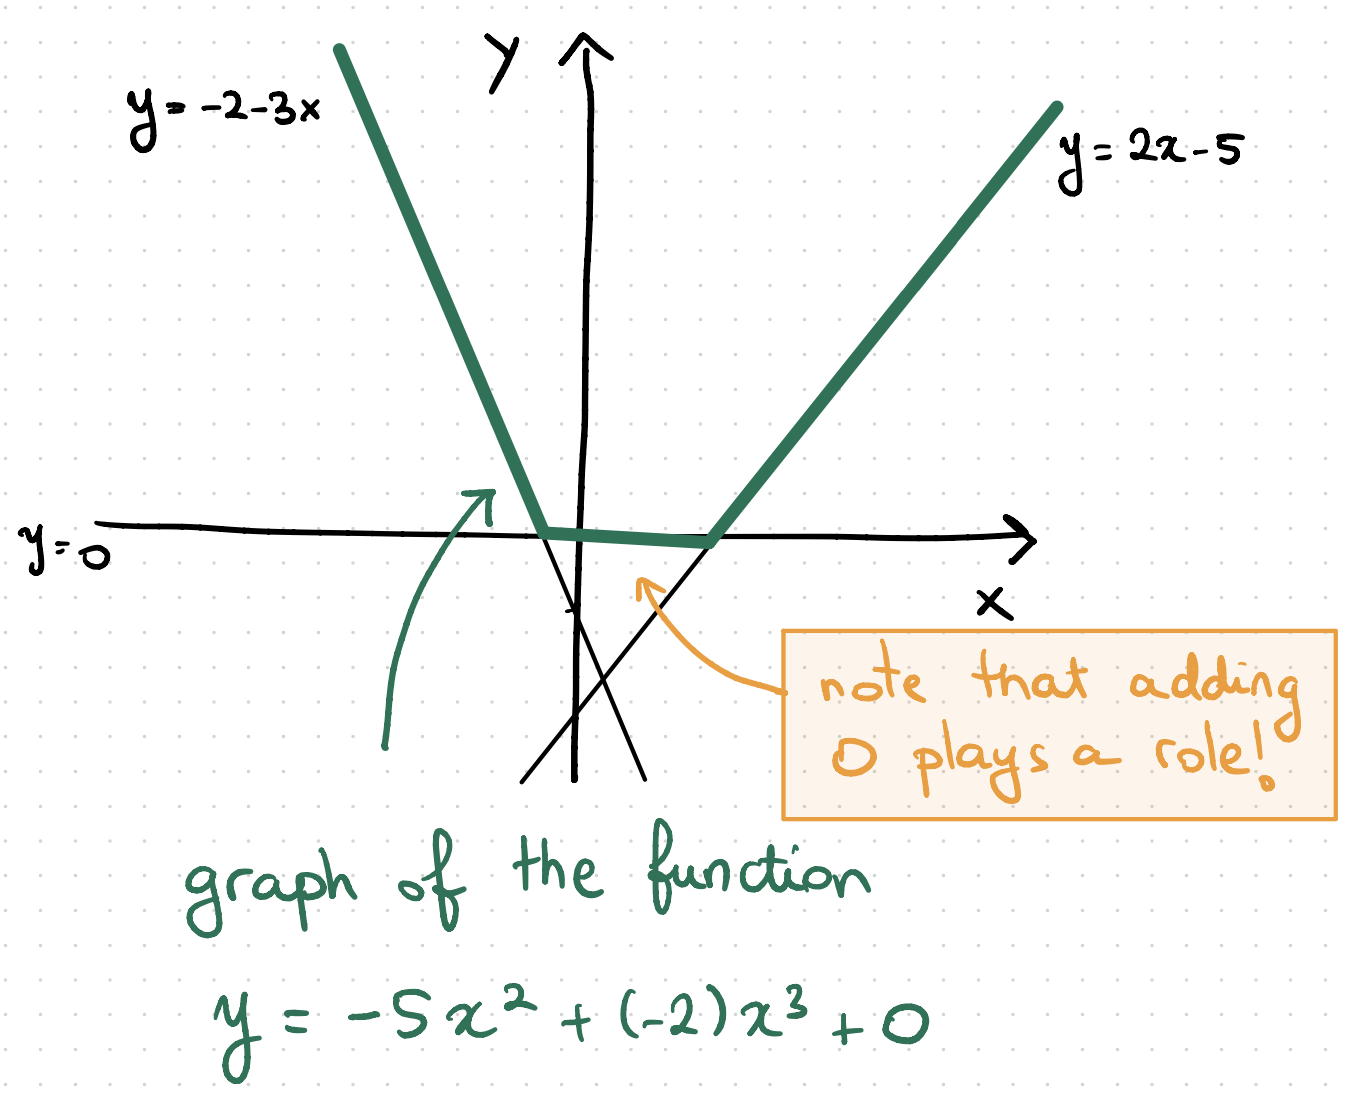
\includegraphics[width=0.5\textwidth]{figs/fig3-1RenzoNotes3.png}
        %\caption{This is the caption.}
        \label{fig:3.1-ConvPLFunc}
    \end{figure}

    Observe that this function is indeed convex, and it fulfills all of the previously stated properties. 
\end{Ex}

In fact, the map from $\bT[x]$ to convex, affine piecewise linear functions with \emph{finitely} many distinct regions of linearity is surjective. If we do not want to take the finiteness condition into consideration, we must amplify the domain to tropical Laurent series.\par 
A small measure of care should be taken here because there are multiple tropical polynomials which map to the same function.

\begin{Ex}
    Consider 
    $$p_1=x+\frac{1}{x}+0\text{ and }p_2=x+\frac1x-2.$$
    In our tropical world, these are
    $$\max(x,-x,0),\quad\max(x,-x,-2),$$
    which both $|x|.$
    \begin{figure}[h!]
        \centering
        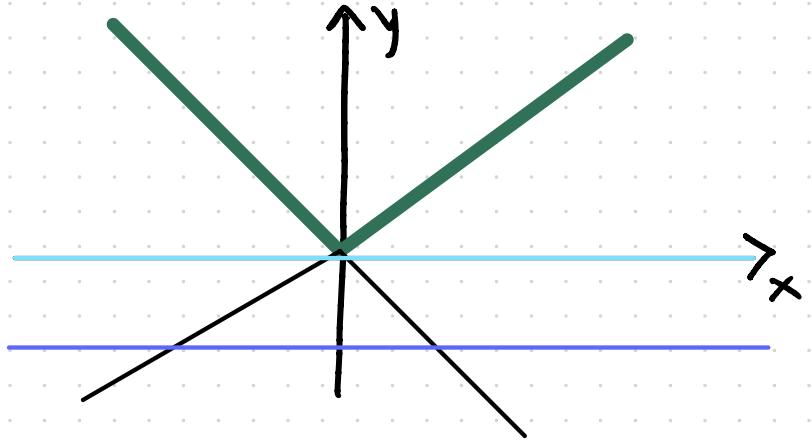
\includegraphics[width=0.5\textwidth]{figs/fig3-2RenzoNotes3.png}
        \caption{Failure of injectivity as both functions map to $|x|$ with $y=0$ and $y=-2$ shown.}
        \label{fig:3.2-InjectivityFailure}
    \end{figure}
    Adding something which is smaller than the minimum value of the function does not change it in general. This added element also need not be a constant. In the previous example, the the monomial $(-4)\odot x^{\odot 1}$ is smaller than any of the linear functions, so its addition changes nothing.
\end{Ex}

Now that we have defined polynomials, we seek a tropical interpretation of roots of polynomials. It does not make sense to say "values of $x$ for which $p(x)= - \infty$, and solving for $0$ also does not help, as in this context, $0$ is just another number/function. Thus, to talk about the roots, we will start with a purely combinatorial definition. 

\begin{Def}
    Given a polynomial $p\in\bT[x]$ of degree $d$, we say the following:
    \begin{itemize}
        \item $-\infty$ is a root of $p$ if the slope of the corresponding affine piecewise linear function is non-zero for $x\ll 0$.
        \item $x_0\in\bR$ is a root of $p$ if $p'(x_0),$ the derivative of the corresponding piecewise linear function, is undefined. Notice that the derivative is undefined only when there is a change in slope.
    \end{itemize}
    We say that the \term{multiplicity} of $x_0$ is the difference between slopes across $x_0$. If $-\infty$ is a root, then its multiplicity is equal to the slope of the associated function for $x\ll 0$.
\end{Def}

\begin{Ex}
    Consider the polynomial $x^{\odot2}\oplus1\odot x^1\oplus 0=\max(2x,x,0)$.
    \begin{figure}[h!]
        \centering
        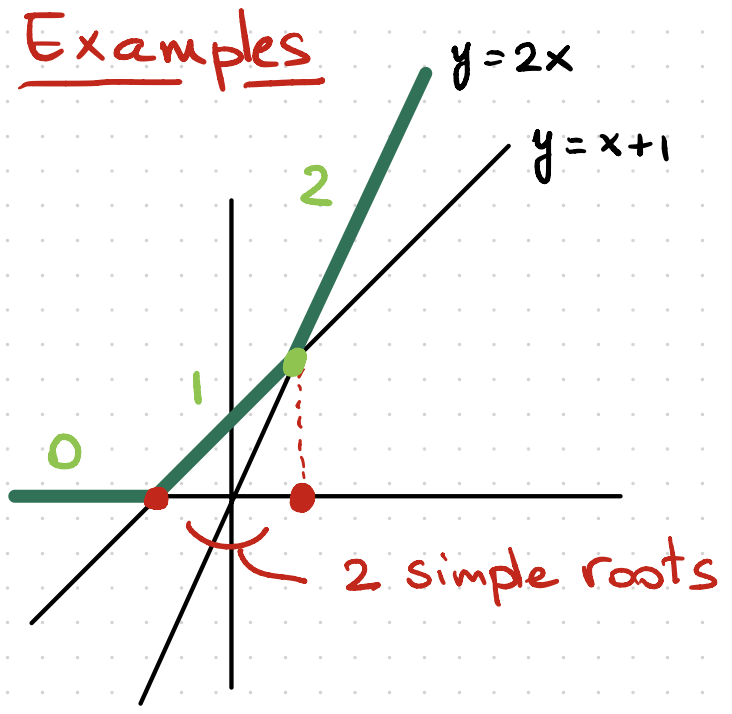
\includegraphics[width=0.5\textwidth]{figs/fig3-3SimpleFiniteRootsTropicalPolynomial.png}
        %\caption{}
        \label{fig:3.3-SimpleFiniteRoots}
    \end{figure}
    
    We can see that there are changes in slope at $x_1=-1$ and $x_2=1$. The number of roots coincides with the degree of the polynomial as in the usual sense.
\end{Ex}

\begin{Ex}
    If we remove the zero (recall that zero is not the additive identity), the polynomial we have instead is $x^{\odot2}\oplus1\odot x^1=\max(2x,x)$.
    \begin{figure}[h!]
        \centering
        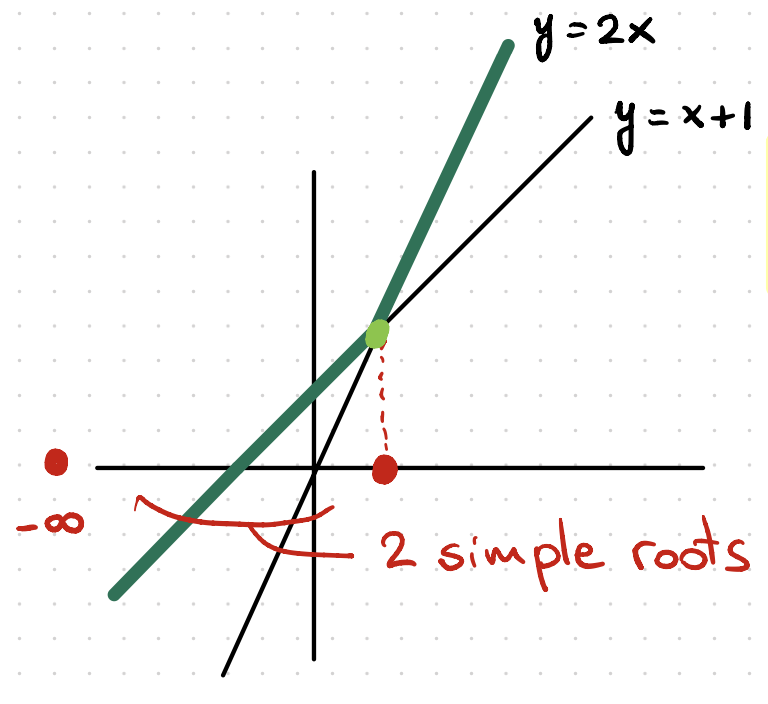
\includegraphics[width=0.5\textwidth]{figs/fig3-4SimpleRootsTropicalPolynomial.png}
        %\caption{}
        \label{fig:3.4-OneFiniteRootOneInfiniteRoot}
    \end{figure}

    Now one of the roots is still $x=1$, but remember that if the slope is non-zero when $x\ll 0$, then $-\infty$ is a root of $p$. This is the case here because the slope is $1$ as $x\to-\infty$. Once again, we have two roots, $x_1=-\infty$ and $x_2=1$.
\end{Ex}



\begin{Def}
    We now define what it means for a tropical root to have multiplicity.
    \begin{itemize}
        \item If $- \infty$ is a root of $p(x)$, its multiplicity is equal to the slope of $f_p(x)$ for $x<<0$.
        \item If $x_0\in\bR$ is a root of $p(x)$, its multiplicity is the difference in slopes across $x_0$. In other words, the multiplicity of the root is equal to the difference in the two extremal positions where the $\max$ is attained.
    \end{itemize}
\end{Def}

Note, if we accept Laurent polynomials, then the multiplicity of $-\infty$ is equal to the slope towards $- \infty$.


\begin{Ex}
    Let us now change a sign in one of our coefficients. Consider $x^{\dot2}\oplus-1\odot x^1\oplus0$. But what is tropical subtraction? Let us convert this slowly into what it's supposed to be:
    $$x^{\odot2}\oplus-1\odot x^1\oplus0=(x\odot x)\oplus(-1)\odot x\oplus0=(2x)\oplus(x\oplus(-1))\oplus0=\max(2x,x-1,0).$$
    \begin{figure}[h!]
        \centering
        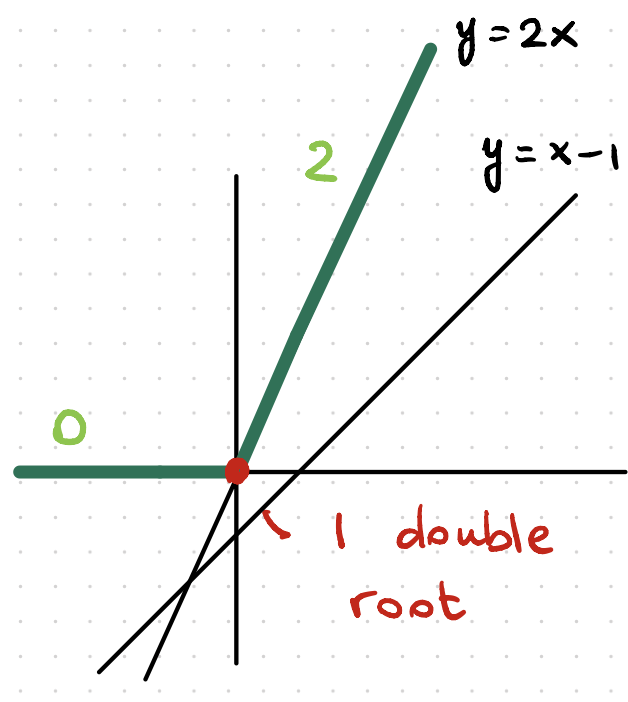
\includegraphics[width=0.5\textwidth]{figs/fig3-5DoubleRootTropicalPolynomial1.png}
        %\caption{}
        \label{fig:3.5-DoubleRoot1}
    \end{figure}

    Observe that because the line $y=x-1$ is below our graphs, it does not interfere with the calculation of our zeroes. The only place where a change in sign occurs is at $x=0$. The slope on the right is $2$, and the slope on the left is $0$, so we say that the multiplicity is $2-0=2$.
\end{Ex}


\begin{Ex}
    In a similar fashion, $x^2+0$ also has a double root at $x=0$.
    \begin{figure}[h!]
        \centering
        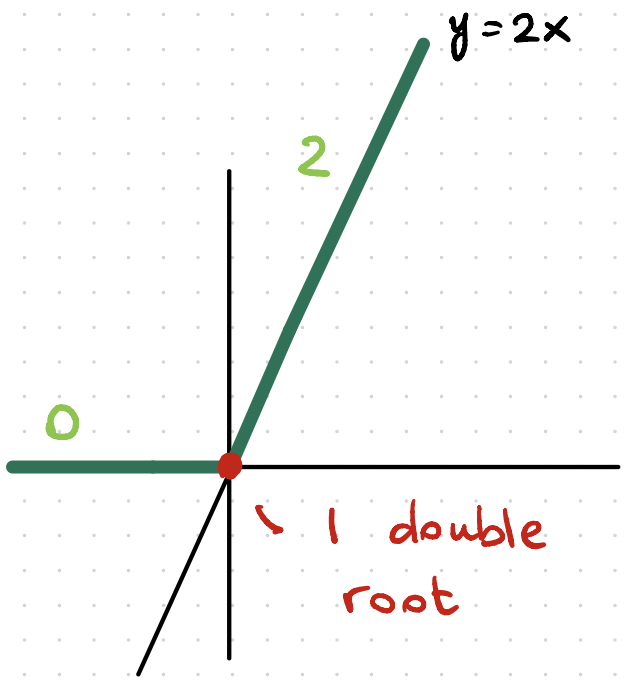
\includegraphics[width=0.5\textwidth]{figs/fig3-6DoubleRootTropicalPolynomial2.png}
        %\caption{}
        \label{fig:3.6-DoubleRoot6}
    \end{figure}
    
    There is only one change in slope at $x=0$, and the difference in slopes is $2$.
\end{Ex}



\begin{Lem}
For a tropical polynomial $p$, a finite $x_0$ is a root of $f$ if and only if when we write the function as a $\max$ of linear functions, the maximum value is obtained at least twice at $x_0$.\par 

\end{Lem}

This should be more or less obvious. A root means that we have an intersection of two lines which are above all the others.


\begin{lemma}
    Only $-\infty$ can have a pole (root with negative multiplicity) due to concavity.
\end{lemma}

As per usual, some questions arise:
\begin{significant}
    \begin{itemize}
        \item Which functions have only one simple zero at $-\infty$?
        \item What would a function with an order two zero at $-\infty$ look like?
    \end{itemize} 
\end{significant}

\begin{Ej}
    Do the following:
    \begin{itemize}
        \item Is it possible for a function to have only a simple zero at $-\infty$? Provide an example of function with one simple zero at $-\infty$ or prove that such function cannot exist. 
        \item Do functions with zeroes at $-\infty$ have infinite order at such a zero, or is the order arbitrarily high? If a function has a zero with finite order at $-\infty$, provide an example of a function with a double zero at $-\infty$. Otherwise, prove that such functions have infinite order at that zero.
    \end{itemize}
\end{Ej}

\subsection{Factorization of Tropical Polynomials}

How do we know that the notions of roots are natural or useful?

Suppose a polynomial $p\in\bT[x]$ has roots $a_k$ with multiplicity $m_k$. Then we may factor $p$ as a product of linear polynomials: 
$$p(x)=c_0\bigodot(x\oplus a_k)^{m_k}.$$
This $p$ is the affine piecewise-linear function, not the formal object. And so, in a sense, $\bT$ is algebraically closed. Instead of proving this, we will simply sketch the proof to get an idea of how things work with a couple of examples.\par 
The basic idea of the proof is that we check that product does define a piecewise-linear function with the right slopes, so that $c_0$ then gives the translation factor.
\begin{Ex}
First, let us deal with the case where $-\infty$ is not a root. Consider the polynomial 
$$p(x)=(-1)\oplus(-1)\odot x\oplus(-4)\odot x^{\odot4}=\max(-1,x-1,4x-4).$$
Remember, as in the case of real polynomials, the square and cube terms are still present. The coefficient that goes along with them is simply $-\infty$. We can graph the polynomial in order to better see the roots:
\begin{figure}[h!]
    \centering
    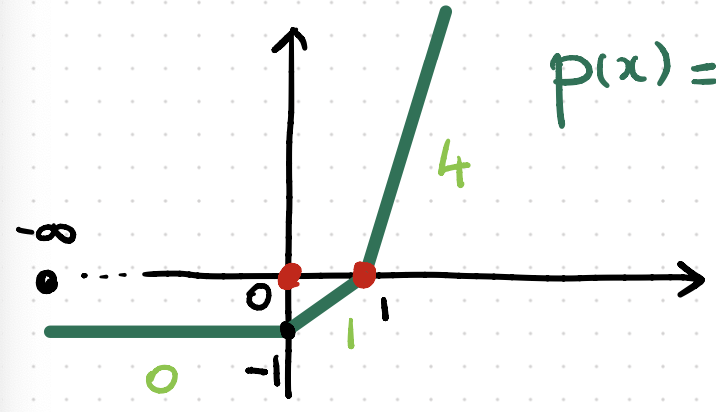
\includegraphics[width=0.5\textwidth]{figs/fig4-1-InfinityNotRoot.png}
    \caption{Graph of $p(x)$ with roots shown}
    \label{fig:4.1-InfinityNotRoot}
\end{figure}

The points where there is a change in slope are $a_1=0$ and $a_2=1$. Their multiplicities are $1-0=1$ and $4-1=3$ respectively. We may write $p$ as 
$$p(x)=c_0\odot(x\oplus 0)\odot(x\oplus 1)^{\odot3}=c_0+\max(x,0)+\max(3x,3).$$
Whatever function we have, we can write it as the sum of three terms. So let us subdivide the tropical line in order to see which terms go where.
\begin{table*}[h!]
    \centering
    %\arraystretch{1.3}
    \begin{tabular}{rrrr}\toprule
        $x\leq 0$ & $0\leq x\leq 1$ & $1\leq x$\\ \midrule
        $c_0$& $c_0$&$c_0$\\
        $0$&$x$ & $x$\\
        $3$& $3$ & $3x$\\ \midrule
        $c_0+3$&$c_0+3+x$&$c_0+4x$\\
   \bottomrule
    \end{tabular}
    \legend{Behavior of $p(x)$ across $\bT$}
    \end{table*}

    The constant $c_0$ can be determined by plugging in $x=-\infty$. We can see that 
    \begin{align*}
        p(-\infty)&=(-1)\oplus(-1)\odot (-\infty)\oplus(-4)\odot (-\infty)^{\odot4}=-1\\
        &=c_0\odot(-\infty\oplus 0)\odot(-\infty\oplus 1)^{\odot3}=c_0\odot0\odot 1^{\odot 3}.
    \end{align*}
    This gives us the equation $c_0+0+3=-1$, which leads us to $c_0=-4$. With this, we verify that 
    $$p(x)=\begin{cases}
        -1&x\leq 0\\
        x-1&0\leq x\leq 1\\
        4x-4&1\leq x
    \end{cases}$$
    So, in this case, $c_0=p(-\infty)-\sum m_ka_k\in\bR$.
\end{Ex}

\begin{Ex}
    We now explore the case where $-\infty$ is a root or a pole. The argument will essentially be the same with a small modification.\par 
    Consider the function $\frac{1}{x}\oplus x$.
    \begin{figure}[h!]
        \centering
        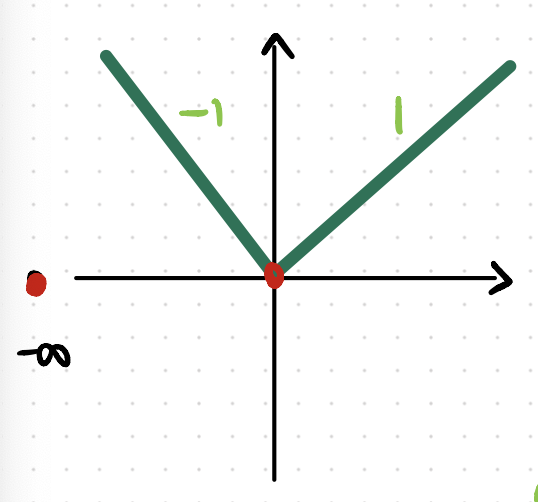
\includegraphics[width=0.5\textwidth]{figs/fig4-2RootAndPoleProof.png}
        %\caption{}
        \label{fig:4.2-RootAndPoleProof}
    \end{figure}
    We have $-\infty$ as a pole of order $1$, and $0$ is a root of order $1-(-1)=2$. So, this can be factored as 
    $$p(x)=c_0\odot(x^{-1})\odot(x+\oplus 1)^2,$$
    and even if $-\infty$ does not give us a particular value for the function, we can still find $c_0=0$ from the equation $p(0)=0$.\par 
    If, on the other hand, we have a negative slope, then we have a zero at $-\infty$. Consider the function $p(x)=x+x^2$:
    \begin{figure}[h!]
        \centering
        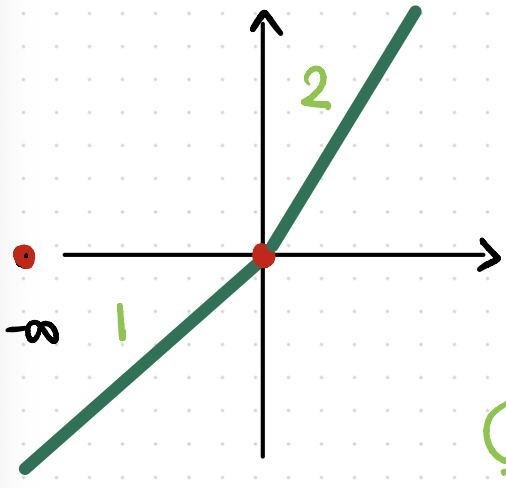
\includegraphics[width=0.5\textwidth]{figs/fig4-3RootsForProof.png}
        %\caption{}
        \label{fig:4.3-RootsForProof}
    \end{figure}

    This function has two simple roots at $-\infty$ and $0$. We may factor it as 
    $$p(x)=c_0\odot(x\oplus-\infty)\odot(x\oplus 0).$$
    Even if $p(-\infty)=-\infty,$ we can plug in $0$ to get $0$ back in order to get $c_0=1$.
\end{Ex}

\subsection{Correspondence Theorems}
Recall the maps
$$
\left\lbrace 
\begin{aligned}
    &T_t\: \bC\to\bT\quad(\text{with }\max),\\
    &\val\: \bC\set{\set{t}}\to\bT\quad(\text{with }\min).
\end{aligned}
\right.
$$
If we consider a polynomial 
$$p(X)\in\bC[X]\word{or}p(x)\in\bC\set{\set{t}}[X],$$
then we can produce a tropical polynomial as follows:

\begin{enumerate}[i.]
    \item Apply $T_t$ or $\val$ to the coefficients.
    \item Perform tropical operations.
\end{enumerate}

We expect that if $r\in\bC$ or $r\in\bC\set{\set{t}}$ is a root of $p$, then $\lim_{t\to\infty}T_t(r)$ will be a root of the new polynomial.\par
We can also work the other way around. Given $p\in\bT[x]$, we can lift the coefficients to $\bC$ or the Puiseux series via the above maps. We can find the roots of the corresponding polynomials in $\bC[x]$ or $\bC\set{\set{t}}[x]$, and then the image of those roots via $T_t$ or $\val$ are the tropical roots of $p(x)$.

\begin{Ex}
    Consider the polynomial $p(x)=2\odot x\oplus3\in\bT[x]$. We wish to construct a polynomial in $\bC[x]$ which tropicalizes to $p$. Take the polynomial 
    $$q(x)=t^2X+t^3\in\bC[x],\quad t>0.$$ 
    We could certainly add phase as $e^{i\te}$ to the $t^k$'s, but that will not change anything. Taking the logarithm of the coefficients, we get 
    $$t^2\mapsto 2\word{and}t^3\mapsto 3.$$ 
    Then, switching to tropical operations, we have
    $$t^2X+t^3\xrightarrow[]{\Trop}2\odot X\oplus 3,$$ 
    which was our original polynomial $p$.\par 
    Additionally, if we solve the equation $q=0$, we obtain the root $X=-\frac{t^3}{t^2}=-t$. Now $\log_t|-t|=1$. Lo and behold, this is the same root of $p(x)$! 
    \begin{figure}[h!]
        \centering
        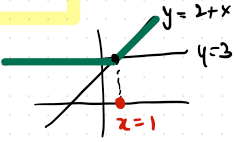
\includegraphics[width=0.5\textwidth]{figs/fig4-4CorrespondenceRoots1Example.png}
        \caption{Root of $p(x)$ in correspondence with $-t$ of $q(x)$}
        \label{fig:4.4-CorrespondenceRoots1Example}
    \end{figure}
\end{Ex}

However, we should be skeptical since this was only an example of a linear polynomial. Let us increase the degree and see what happens to hopefully eventually show that this correspondence holds in its entirety.

\begin{Ex}
    Consider the polynomial
    $$q(X)=X^2+t^2X+1\in\bC[X]\xrightarrow[]{\Trop}p(x)=x^{\odot2}\oplus 2\odot x\oplus 0.$$
    We can identity the roots of $p$ as $-2$ and $2$. However, we may find it difficult to interpret the roots of $q$ as roots of $p$. Observe that, using the quadratic formula, we may derive those to be:
    $$X_{1,2}=\frac{-t^2}{2}\pm\frac{\sqrt{t^4-4}}{2}=\frac{-t^2}{2}\left(1\pm\sqrt{1-\frac{4}{t^4}}\right).$$
    Even if taking the logarithm seems hard, notice that we are not interested in the logarithm itself, just the limit! Observe that 
    $$\lim_{t\to\infty}\log_t\left|\frac{-t^2}{2}\left(1+\sqrt{1-\frac{4}{t^4}}\right)\right|=2+\lim_{t\to\infty}\frac{1}{\log(t)}\log\left|\frac{1}{2}\left(1+\sqrt{1-\frac{4}{t^4}}\right)\right|.$$
    The quantity on the right tends to $1/\infty$, which collapses to zero, so the logarithm only has $1$ as its argument. Overall, we find one of our original roots, $2$! The next limit has a different sign, so it is not as direct. We may calculate that limit as follows:
    $$\lim_{t\to\infty}\log_t\left|\frac{1}{2}\left(1-\sqrt{1-\frac{4}{t^4}}\right)\right|\approx\lim_{t\to\infty}\log_t\left|\frac{1}{2}\left(1-\left(1-\frac{4}{2t^4}\right)\right)\right|=\lim_{t\to\infty}\log_t\frac{1}{t^4}=-4.$$
    So, for the negative root, we would actually obtain $2-4=-2$, which is the other root of our polynomial.
    \begin{figure}[h!]
        \centering
        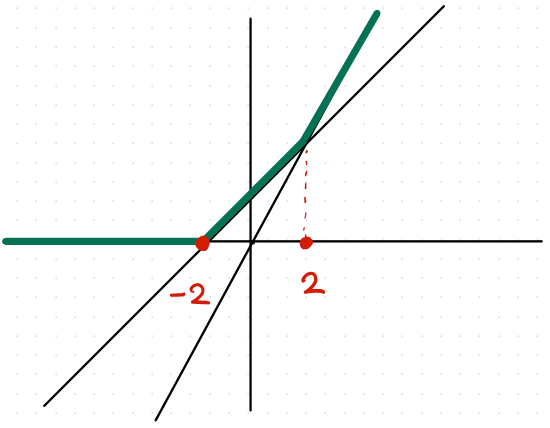
\includegraphics[width=0.5\textwidth]{figs/fig4-5CorrespondenceRoots2Example.png}
        \caption{Indeed the roots of $q$ correspond with $p$'s}
        \label{fig:4.5-CorrespondenceRoots2Example}
    \end{figure}
\end{Ex}







\section{Interim 2}

\begin{Def}
    If $q(x)=\sum a_kx^k\in\bC[X]$ or $\bC\set{\set{t}}[x]$, then the \term{tropicalization} of $q$ is 
    $$\Trop(q)=\sum T_{t\to\infty}(a_k)x^k$$
    or respectively with the valuation. In this case, we omit the notation for tropical operations but the sum and product are indeed tropical.
\end{Def}

\begin{Th}
For a polynomial $q$, $r_k$ is a root of $q(x)$ with multiplicity $m_k$ if and only if $T_{t\to\infty}(r_k)$ is a root of $\Trop(q)$ of multiplicity $m_k$.
\end{Th}

In the univariate case, we may prove the theorem using the following lemmas.

\begin{Lem}
$\Trop$ is a multiplicative function on polynomials. That is,
$$\Trop(pq)=\Trop(p)\Trop(q)\word{for}p,q\in\bC[x].$$
\end{Lem}

\begin{Lem}
The roots of $\Trop(p)\Trop(q)$ are the union of the roots of the factors. If a root is repeated, then the multiplicities are added.
\end{Lem}

\begin{Ej}
Prove the preceding lemmas and then conclude the theorem as a result.
\end{Ej}

Otherwise, we may prove the correspondence theorem in a different way. This is more conducive to a higher number of variables. This is helpful, as in higher dimensions we do not have a fundamental theorem of algebra. But, in this case, the most convenient perspective is the valued field perspective, so let us swtich to that point of view and interpret 
$$x\oplus y=\min(x,y).$$

\begin{Th}
Let $q\in\bC\set{\set{t}}[x]$. Then $r\in\bC\set{\set{t}}$ is a root of $q$ if and only if $\val(r)\in\bT\cap\bQ$ is a root of $\Trop(q)$.
\end{Th}

\begin{ptcbp}
Let us begin by considering a root $r$ of $q$. Then $q(r)=0$, which means that 
$$a_0+a_1r+\dots+a_dr=0.$$
This is formal sum of monomials which, in order to vanish, must have at least two of the monomials reaching a minimum order of vanishing to cancel. This is equivalent to $\val(r)$ being a root of $\Trop(q)$. \par %%REVIEW
The other direction is substantially more difficult, as it is an instance of a realizability question. We have two cases; either $r$ is a finite root or $r=\infty$. We will assume that $r$ is finite and proceed with a proof by example. 
\end{ptcbp}

\begin{Ex}
    Consider the polynomial 
    $$q(x)=tx^3+x^2+x+t\To\Trop q(x)=1\.x^3+x^2+x+1.$$
    \begin{figure}[h!]
        \centering
        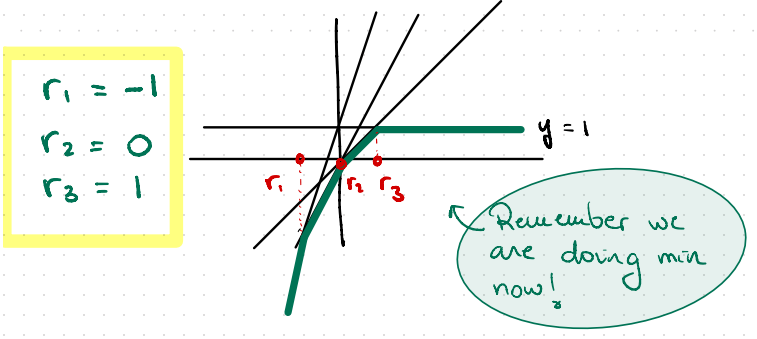
\includegraphics[width=0.85\textwidth]{figs/fig5-1RealizabilityExampleProof.png}
        \caption{Tropicalization of $q$ in $\min$ convention}
        \label{fig:5.1-RealizabilityExampleProof}
    \end{figure}

    The roots of this polynomial are $-1,0$, and $1$. We will now find a root $r_1\in\bC\set{\set{t}}$ of $q$ with $\val(r_1)=r_1$. For this to happen, we require
    $$r_1=yt^{-1}+z\word{where}y\in\bC,\word{and}z\in\bC\set{\set{t}},\ \val z>r_1.$$
    We now plug $r_1$ into $q$ and obtain
    \begin{align*}
        q(r_1)&=t(yt^{-1}+z)^3+(yt^{-1}+z)^2+(yt^{-1}+z)+t\\
        &=\un{y^3t^{-2}}+3y^2zt^{-1}+3yz^2+z^3t+\un{y^2t^{-2}}+2yzt^{-1}+z^2+yt^{-1}+z+t.
    \end{align*}
    Extracting the coefficients, we get $y^3+y^2=0$, which means that $y=-1$. Plugging this back into our expression as $y$, we get 
    $$3zt^{-1}-3z^2+z^3t-2zt^{-1}+z^2-t^{-1}+z+t=tz^3-2z^2+(t^{-1}+1)z+(-t^{-1}+t).$$
    Tropicalizing (\red{is it actually or is it the reverse operation?}), we get 
    $$1\.z^3+z^2+(-1)z+(-1)$$
    which has as a root $1>-1$. So,
    $$z=y+z_1\word{with}y\in\bC,\quad z_1\in\bC\set{\set{t}}.$$  
    \begin{figure}[h!]
        \centering
        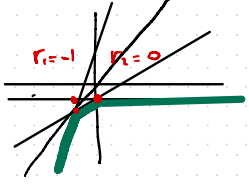
\includegraphics[width=0.5\textwidth]{figs/fig5-2EndOfProofFiniteCase.png}
        \caption{I don't know what this is}
        \label{fig:5.2-EndOfProofFiniteCase}
    \end{figure}
    \red{ASK MAPLE CODE}
\end{Ex} 

The question now is: how do we turn this idea into a formal proof?
\begin{enumerate}[i.]
    \item We do one root at a time, starting with the rightmost one.
    \item Observe that if $r$ is a tropical root and $\al=yt^r$ with $y$ chosen so cancellation happens, then denoting $\tilde{q}$, $q$ without the $x^0$ term:
    $$\Trop(q(x+\al))>\Trop(\tilde{q})\oplus\Trop(q(\al)).$$
    \item Finally, we iterate and check that the sequence of $r_i$'s goes to $\infty$.
\end{enumerate}




\subsection{Combinatorialization of Root Finding}

We momentarily convert to the max convention. Let us consider $p(x) = \sum\limits_{i=0}^d a_i \odot x^{\odot i}$. Can we develop a systematic and simple way to say how many roots, with what multiplicity, and what equations to solve?\par 
Indeed, $p(x) = \max_i \{a_i + ix\}$. There are $d+1$ lines $y= a_i + ix$. It is a finite process to intersect every pair of these lines, and then to compare the corresponding heights of each function to find the max. To make root finding more efficient, we work from left to right.\par
The left-most root can be found via
$$\min\left(\frac{a_0-a_k}{k}\right)=\text{achieved by }k\text{ such that }\frac{a_0-a_k}{k}\text{ is maximized}.$$
In other words, we are looking for the largest slope:
\begin{figure}[h!]
    \centering
    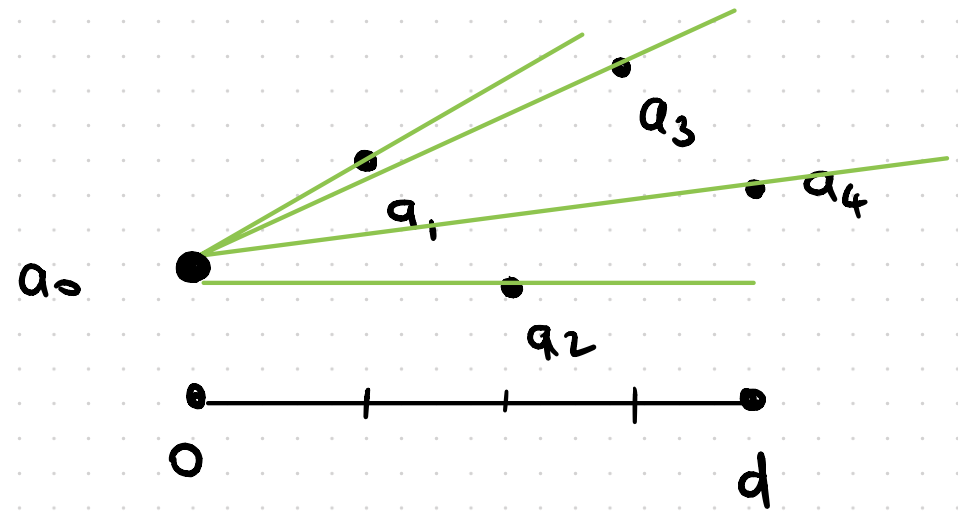
\includegraphics[width=0.5\textwidth]{figs/fig6-1BiggestSlope.png}
    \caption{Difference of coefficients as slopes}
    \label{fig:6.1-BiggestSlope}
\end{figure}


This gives us $a_j$ for our first root. Our next root is to the right of $a_j$ because the corresponding line has a larger slope than the preceeeding lines, and the preeceding lines have an intersection, and are thus no longer considered in our root finding. So we use that as our next starting point, and we continue on.
We then get the following algorithm:
\begin{enumerate}[i.]
    \item Let $p_k=(k,a_k)\in\bonj{0,d}\x\set{-\infty}\cup\bR$.
    \item Now $\Sg$ is the convex hull of the points $\set{p_k\:\ k\in[d]}$. We may divide the region into $\Sg^+$ and $\Sg^-$.
    \item Call $q_i=\pi(p_i)$ for $p_i$'s that for the vertices of $\Sg^+$.
\end{enumerate}

Following this algorithm, we have that
\begin{itemize}
    \item [A)] The roots of $p(x)$ are in bijection with the complement of the projections, i.e. the subdivisions of the Newton polytope.
    \item [B)] The value of the root corresponding to a given segment $(i,j)$ is found by solving the equation $a_i + ix = a_j  +jx$.
    \item [C)] The multiplicity of the root is equal to the length of the segment.
\end{itemize}



\begin{Ex}
    Take for example the polynomial 
    $$p(x)=0+1\.x+1\.x^2+x^3+2\.x^4+1\.x^5.$$
    We now place the points in our diagram and project:
    
    \begin{figure}[h!]
        \centering
        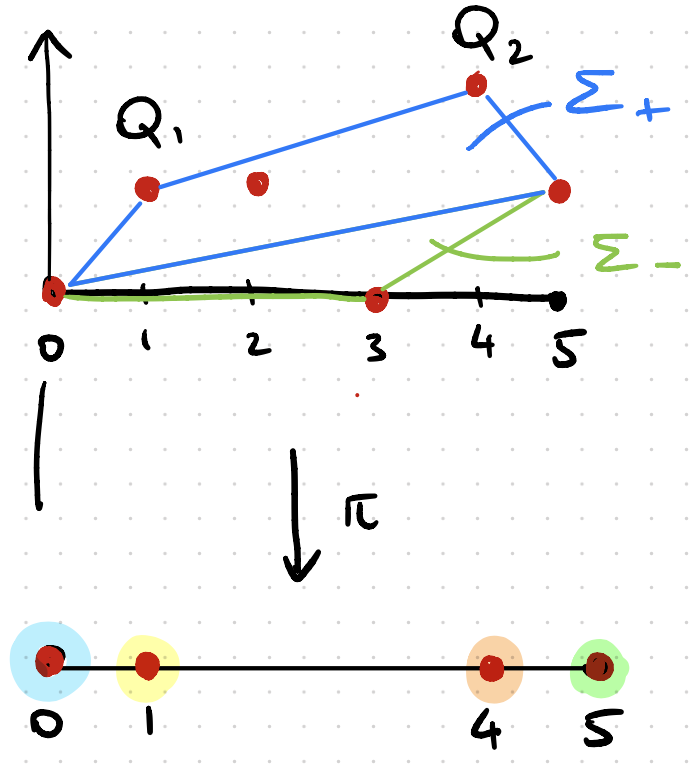
\includegraphics[width=0.5\textwidth]{figs/fig6-2CombinatorializationExample.png}
        \caption{Root finding for $p(x)$}
        \label{fig:6.2-CombinatorializationExample}
    \end{figure}

    From this, we deduce that there are two simple roots and one triple root. This comes from the equations
    $$
    \left\lbrace
    \begin{aligned}
        &0=x+1&\To x=-1\\
        &x+1=2+4x&\To x=-1/3\\
        &2+4x=1+5x&\To x=1
    \end{aligned}
    \right.
    $$
\end{Ex}



\subsection{Grobner}

Let $K$ be a field with valuation, such as $\CC\{\{t\}\}$. Then we will call$$
\left\lbrace
\begin{aligned}
    &R_K\subseteq K=\text{ elements with non-negative valuation}\\
    &\lie{m}\subseteq R_K=\text{ elements with positive valuation}
\end{aligned}
\right.
$$
Notice that $\quot{R_K}{\lie{m}}$ is a residue field. 
$$\lie{m}=\bigcup_nt^{1/n}\bC\bonj{\bonj{t^{1/n}}}\subseteq R_K=\bigcup_n\bC\bonj{\bonj{t^{1/n}}}\subseteq\bC\set{\set{t}},\word{and}\quot{R_K}{\lie{m}}=\bC.$$

Tropical polynomials form a Gr\"obner complex\footnote{What are Gr\"obner complexes? To see in interim.}.

\begin{Def}
    Given $q\in K[x]$ and $w\in\bT$, the \term{initial form} of $q(x)$ with respect to $w$ is a polynomial in $K[x]$that records the part of $q$ that has lowest order when $\val(x)=w$.
\end{Def}

\begin{Ex}
    Let us consider the polynomial 
    $$q(x)=t^{-4}+\sqrt{2}x+3t^2x^2.$$
    Suppose we picked a valuation $val(x) = -3$. We can then ask for the valuation of the individual terms. Then
    $$t^{-4}\to -4,\quad \sqrt{2}x\to-3,\quad 3t^2x^2\to -4,\word{so}w=-3.$$
    We may construct the initial form as $I_wq=1+3x^2$, but formally this is $\bonj{t^4(q(t^{-3}x))}_{t=0}$. In general, if $W=\Trop q(w)$, then 
    $$I_wq=\bonj{t^{-W}(q(t^{w}x))}_{t=0}.$$
\end{Ex}




\subsubsection{Gr\"obner Complex of $q(x)$}

Polyhedral decomposition of $\bR$ (in the case of a valuation space, we can also add in $\infty$, but it usually is left out) is induced by the equivalence relation
$$w_1\sim w_2\iff In_{w_1}q=In_{w_2}q\footnote{Does this refer to initial form?}.$$

\begin{Ex}
    Consider the polynomial 
    $$t^2+\sqrt2x+3t^2x^2.$$
    Each monomial maps\footnote{Through what? The valuation?} to $2,w,$ and $2+2w$ respectively.
    \begin{figure}[h!]
        \centering
        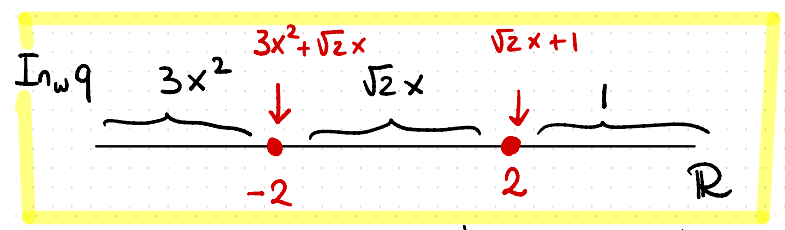
\includegraphics[width=0.5\textwidth]{figs/fig6-3-InitialFormExample.png}
        \caption{Initial form determination and roots}
        \label{fig:6.3-InitialFormExample}
    \end{figure}

    So the tropical roots are the locus where the initial form is not a monomial.
\end{Ex}


\begin{define}
    The complement of the locus of $w$ such that $In_W q$ is a monomial is called the \term{Gr\"obner complex} of $q(X)$.
\end{define}

The Gr\"obner complex of $q(X)$ is equal to the roots of $trop(q(x))$.


\section{More Variables}


Let $p(x,y)= \sum a_{ij} \odot x^i\odot y^j$ be a tropical polynomial in two variables. 

\begin{define}
    Define a \term{tropical curve} $V(p)$ to be either
    \begin{enumerate}
        \item the locus in the domain of piecewise-linear $p$ where $p$ is not linear, or
        \item $\{(x,y)\; |\; \max(a_{ij} +ix+jy)$ is attained and is $>1\}$.
    \end{enumerate}
\end{define}

\subsection{Our First Correspondence Theorem}

\begin{Def}
    Given a family of polynomials 
    $$q_t=\sum A_k(t)x^k\in\bC[x]\word{with}t>1,$$
    the \term{tropicalization} of $q_t$ is 
    $$\Trop(q_t)(x)=\sum a_k\odot x^{\odot k},\word{where}a_k=\lim_{t\to\infty}T_t(A_k).$$
    We may also use the $\min$ convention by exchanging the field to Puiseux series and $T_t$ by the valuation.
\end{Def}

\begin{Th}
    If $q(x,y)$ is a polynomial with coefficients over valued field $\CC\{\{t\}\}$ and $trop (q) = p$, then the tropical curve $V(p)$ is equal to the closure of the valuation of the points $\{(val(x), val(y)) \:\; |\; (x,y) \in V(q)\}$.
\end{Th}

We can study structural properties of tropical curves. We get a correspondence statement with subdivisions of Newton polygons, and we get balancing and edge weights.  We will also see the tropical versions of classical plane curve theorems. In particular, we get a tropical Bezout theorem (two projective curves of degree d and e intersect in $d*e$ points) and a tropical degree/genus formula.


\begin{Th}[Correspondence]
    For a polynomial $q_t$, $R_t$ is a root of $q_t$ if and only if $\Trop(R_t)=\lim_{t\to\infty}T_t(R_t)$ is a root of $\Trop(q_t)$.
\end{Th}


This is saying that we have a polynomial, an object in algebraic geometry, and tropical geometry will somehow know about its roots by degenerating it. Then it is easy to find the tropical roots, and there must be certain algebraic roots that map to them. It may not be easy to understand this last map, but at least we have some qualitative information.\par 
We can use the fundamental theorem of algebra to reduce to the linear case, so the first step is to prove the theorem for the case of linear polynomials. We have a couple of lemmas to finish the proof and expand it to the general case:


\begin{Lem}
    $\Trop$ is a multiplicative function on polynomials. That is,
    $$\Trop(pq)=\Trop(p)\odot\Trop(q)\word{for}p,q\in\bC[x].$$
    \end{Lem}
    
This first lemma does not add anything unusual because the tropical product is just the standard addition.

    \begin{Lem}
    The roots of $\Trop(p)\odot\Trop(q)$ are the union of the roots of the factors. If a root is repeated, then the multiplicities are added.
    \end{Lem}

    Essentially what this is saying is that if we have two piecewise-linear functions which change slope at the same place, then the sum will also change slope at the same place. Because the functions are convex, a root can never be cancelled, except possibly $-\infty$.

    \subsection{Higher Dimension}

    We will return to the Puiseux series convention now:
    $$P(X)\in\bC\set{\set{t}}\bonj{X},\ P(R)=0\iff \Trop(P)(\val(R))=0.$$
    The easier direction is to begin with a root of our Puiseux polynomial. Let 
    $$P(X)=\sum A_i(t)X^i,\word{and}\Trop(P)(X)\sum a_i\odot x^i$$
    where $a_i=\val(A_i)$. Let $R=R(t)$ be a root of $P(X)$.\par 
    We know $\val(P(R))=\infty$ because $P(R)=0$. Formally, $\val(P(R))$ should greater than or equal to the minimum of the valuation of each of the monomials evaluated at $R$. In other words,
    $$\min(\val(A_i(t)R^i))=\min_i(a_i+i\val(R))=Trop(P)(R).$$
    Since we know that strict inequality holds, the terms in the formal evaluation with lowest order must cancel. In other words, the minimum is attained at least twice by two different monomials.\par 
    We previously mentioned attaining the minimum twice is the same as being a root.

    \begin{Ex}
        Consider the polynomial $(t^2+7t^3)X+(t^5+t^{27})=Q(X)$. The root here is $R=-\frac{t^5+t^{27}}{t^2+7t^3}$, and its valuation is $5-2=3$. If we plug in something of this form instead of $X$, we get 
        $$Q(-t^3+O(t^4))=(t^2+7t^3)(-t^3+O(t^4))+(t^5+t^{27})=(-t^5)+t^5+O(t^6).$$
        In particular, the first thing that will cancel is the lowest order term, $t^5$. So \emph{two} monomials must have lower order term.
    \end{Ex}

The next thing to consider is whether this process makes sense if we instead begin with a Puiseux series polynomial. If the process ends up being the same, does this mean that tropical geometry over a trivially valued field is uninteresting? That is not the case; this is simply because we are in dimension zero. 

\subsection{Gr\"obner Complexes}

These types of complexes arise in commutative algebra. The setup begins with a valued field, Puiseux series $\bC\set{\set{t}}$, in our case. We can find the ring of integers, the positive valued elements, in our field. These types of functions are regular at $t=0$. Inside this ring, we have the maximal ideal of functions which vanish at zero. If we wish, we can take a quotient to find the residue field, which is a copy of $\bC$.\par 
Every time we are given the data of polynomial $q$ in $\bC\set{\set{t}}\bonj{x}$ plus a choice of a valuation, we can recover the initial form of $q$, which is a polynomial with coefficients in the residue field.\par 
The way to find it is to look at the valuation of each monomial assuming $\val(x)=w$ and then save only the monomials with the smallest valuation and only keep the coefficient in front of the smallest term.

\begin{Ex}
    Consider the polynomial 
    $$q(x)=t^{-4}+t^{2}+\sqrt{2}x+3t^2x^2,$$
    and take $w=-3$. This means that $\val(x)=-3$. Let us now consider the valuation monomial by monomial.\par 
    The term $(t^{-4}+t^{2})$ has valuation $-4$ because there is no $x$. For $\sqrt{2}x$, we have
    $$\val(\sqrt{2}x)=\val(\sqrt{2})+\val(x)=0+(-3)=-3.$$
    Therefore, it has valuation $-3$,and $3t^2x^2$ has valuation $2-6=-4$. We now consider only the first and last terms, as they have the smallest valuation, and extract the coefficients of the smallest terms. In the case of $t^{-4}+t^{2}$, it is the $1$ accompanying the $t^{-4}$ and a $3$ accompanying the last term. So the initial form is 
    $$\operatorname{In}_{-3}(q)=1+3x^2.$$
\end{Ex}

\red{FORMULA for initial form}\par 
We now define an equivalence relation over $(\bR,w)$,
$$w_1\sim w_2\iff In_{w_1}q=In_{w_2}q,$$ 
which separates $\bR$ into two types of equivalence classes:
\begin{itemize}
    \item single points in which the initial form is not a monomial,
    \item open intervals where the initial is a monomial.
\end{itemize}

The Gr\"obner complex of $q(x)$ is equal to the roots of $\Trop(q)(x)$. This is indeed in correspondence with Gr\"obner basis, which is very interesting in higher dimension. 

\subsection{1-dimensional Tropical Geometry}

If we have $p(x,y)$, a tropical polynomial in two variables, then we can define its tropical variety to be $V(p)$:
\begin{itemize}
    \item The locus in the domain where the piecewise-linear function where $p$ is not linear.
    \item The locus of points $(x,y)$ where the $\max$ associated to each monomial is obtained more than once.
\end{itemize}

We will have a correspondence theorem which says that if $q(x,y)$ is a polynomial with coefficients over a valued field and the tropicalization of $q$ is $p$, then 
$$V(p)=\ov{\set{(\val(x),\val(y))\: (x,y)\in V(q)}}.$$
\begin{Ej}
Show that pairs of rational numbers are dense here. \aside{It has to do with the valuation only taking rational numbers.}
\end{Ej}

\subsection{Tropical Lines}

\subsubsection{The $\max$ convention}

If we have a tropical polynomial of degree 1, 
$$p(x,y)=a\odot x\oplus b\odot y\oplus c,$$
we will assume for the sake of drawing pictures that $-\infty\neq a,b,c$. This corresponds to the piecewise-linear function 
$$\max(a+x,b+y,c),$$
and if we set any of these two equations equal to each other, we can see that there are three lines that play a role:
\begin{align*}
    &a+x=b+y\To y=x+(a-b)\\
    &a+x=c\To x=c-a\\
    &b+y=c\To y=c-b
\end{align*}
So this is the locus where two functions are equal to each other. In each of the regions, the maximum is attained by a particular linear function, and the boundary between them is the locus of non-linearity. The point in the middle is $(c-a,c-b)$. 

\begin{figure}[h!]
    \centering
    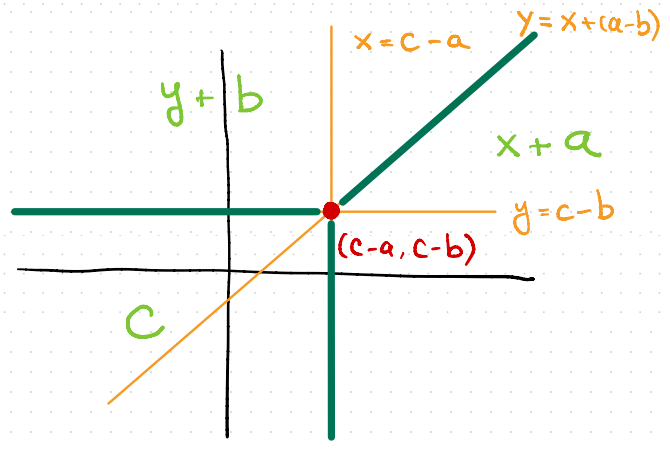
\includegraphics[width=0.5\textwidth]{figs/fig7-1-TropicalLineExample.png}
    \caption{Graph of $p(x,y)=0$ in $\bR^2$}
    \label{fig:7.1-TropicalLineExample}
\end{figure}

In general, tropical lines look like this "tripod," and changing the $a,b,c$ shifts the graph. 

\begin{Ej}
Figure out what happens when a coefficient is $-\infty$.
\end{Ej}

This is analogous to what we have done with tropical univariate polynomials. The tropical line $V(p)$ is the locus of non-linearity of our function:
$$V(p)=\set{(x,y)\in\bR^2\:\ df_p\!\mid\!_{(x,y)}\text{ is not defined}}.$$

\subsubsection{The Case of Puiseux Series}

In this case, lines in the zero loci of polynomials are of the form 
$$p(X,Y)=A(t)X+B(t)Y+C(t)$$
with 
$$a=\val(A),\quad b=\val(B)\word{and}c=\val(C).$$
We let $L=\set{(X,Y)\in\bK^2\:\ p(X,Y)=0}$ be the zero locus and then define
$$\Trop(L)=\ov{\set{(\val(X),\val(Y))\:\ (X,Y)\in L}}\subseteq\bT^2.$$
We may parametrize $p$ in the following way. Let $X=\ga(t)$ with an arbitrary valuation, and then solve for $Y$:
$$Y=\underbrace{\frac{-A(t)}{B(t)}\ga(t)}_{a-b+\val\ga}-\underbrace{\frac{C(t)}{B(t)}}_{c-b}$$ 
\red{ASK RENZO} Depending on the value of $\val\ga(t)$, we may get different values for $\val Y(\ga(t))$. 
\begin{itemize}
    \itemsep=-0.4em 
    \item If $\val\ga(t)>c-a$, then $\val Y(\ga(t))=c-b$.
    \item If $\val\ga(t)<c-a$, then $\val Y(\ga(t))=x+a-b$.
    \item If $\val\ga(t)=c-a$, then $\val Y(\ga(t))$ can be anything above $c-b$. We therefore set 
    $$\ga(t)=\left(-\frac{C(t)}{A(t)}\right)(1+t^{\odot m}),\word{where}m>0.$$
\end{itemize}
The first two items represent a graph of $(a-b)x+(c-a).$\footnote{ask Renzo because I don't understand, page 4 of TG7.}

\begin{Rmk}
If we send $a,b,c,X,$ and $Y$ to their negatives, then $\Trop(L)$ agrees with the previous perspective. Alternatively, we can check that $\Trop(L)$ agrees with the previous perspective but using the $\min$ convention.
\end{Rmk}

\begin{Ex}
    Let us explicitly choose $A,B$ and $C$:
    $$q(X,Y)=t^aX+t^bY+t^c.$$
    Note that $q$'s tropicalization is $p(X,Y)$.
    Points in $V(q)$ can be parametrized as 
    $$X=\al,\quad Y=\frac{-t^a}{t^b}\al-\frac{t^c}{t^b}=-t^{a-b}\al-t^{c-b},\word{where}\al\in\bK^\ast.$$
    Taking valuations of $X$ and $Y$, we get $\Trop(L)$ (but without closing it). Specifically, we are looking at the set 
    $$\Trop(L)=\set{\left(\val(\al),\val(-t^{a-b}\al-t^{c-b})\right)\in\bT^2\:\ \al\in\bK^\ast}.$$
    We can let $\al$ have any valuation we want and, depending on that, we determine the valuation of the binomial $Y$. The possible valuations are 
    $$\val Y=a-b+\val(\al)\word{or}\val Y =c-b,$$
    which are equal when $\val(\al)=c-a$. \red{ASK RENZO ABOUT THIS HOW TO DETERMINE THE CRITERION ABOUT VAL AND STUFF}

    \textbf{Claim: We can obtain any value for $y$, but it must be greater than $c-b$.}
    Let $r\geq 0$ and $\al=-t^{c-a}(1+t^r).$
\end{Ex}

\begin{figure}[h!]
    \centering
    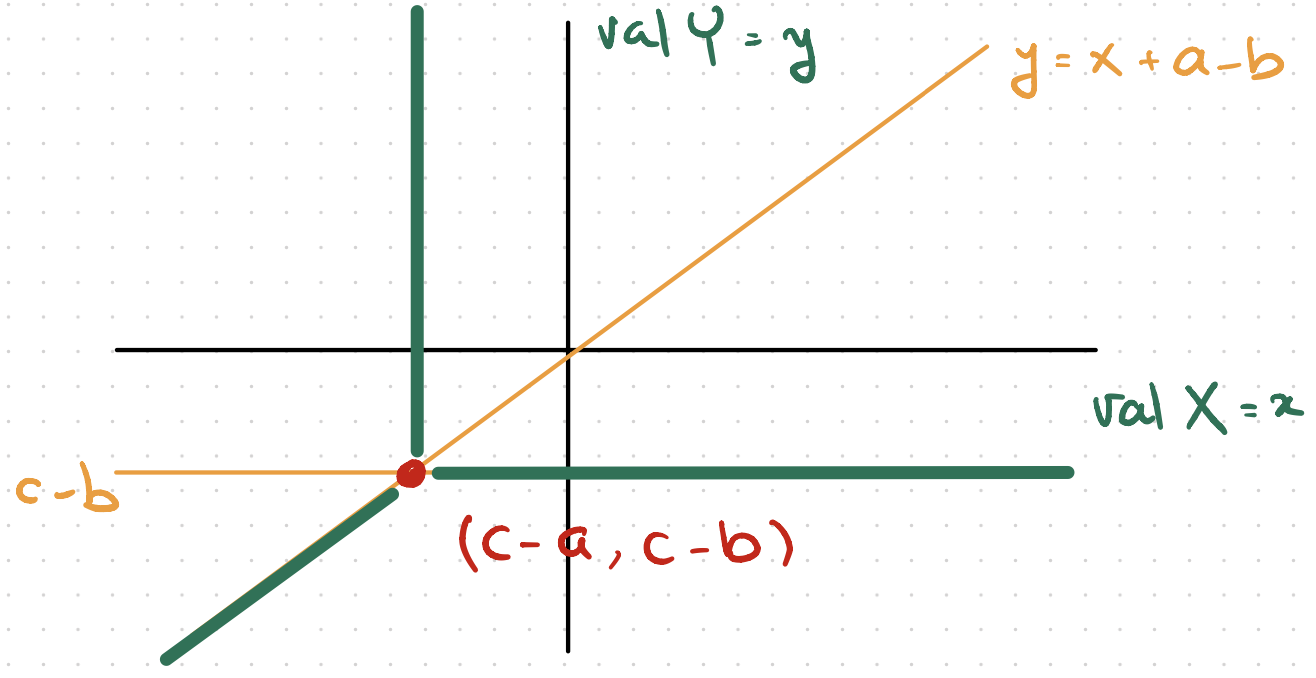
\includegraphics[width=0.5\textwidth]{figs/fig7-2-TropicalLinePuiseuxExample.png}
    \caption{The tropical line from the Puiseux perspective}
    \label{fig:7.2-TropicalLinePuiseuxExample}
\end{figure}

\subsubsection{Glimpse into Amoebas}

Recall that what matters the most is the logarithm base $t$ of our function. So let us continue with 
$$q(x,y)=t^ax+t^by+t^c$$
and play the same game as before. We look for solutions to the equation $q_t=0$ in $\bC^2$, which is a line intersecting the $x$-axis at $-t^{c-a}$ and the $y$-axis at $-t^{c-b}$. Every pair of points $(x,y)$ gives us a pair $(\log_t|x|,\log_t|y|)$. We get the real trace of this when $x,y\in\bR$ can be parametrized with $x=t^\al$ and $y=-t^{a-b+\al}$. We analyze the trace in three intervals. 

To recap, for $p(x,y)$ a tropical polynomial, we can define the variety of $p,$ $V(p)$, which is either the locus of non-linearity of $p$ or the locus where the maximum is attained more than once. Then for $q(X,Y)$ a polynomial, we can tropicalize it.


\subsection{Lines}
Lines are $V(p)$ such that $deg(p)=1$.
Now, to see what happens with tropical lines, consider $p(x,y) = (a \odot x) \oplus (b \odot y) \oplus c$. Assume $-\infty<a<b<c$. Then $p(x,y) = max\{ a+x,b+y,c\}$.

Setting any two equal to each other, we get $a+x=b+y$, $a+x=c$, and $b+y=c$. We get three lines, $y=x+(a-b)$, $x=c-a$, and $y=c-b$.

Every tropical line is of the form of a tripod. Even if we only keep $-\infty< a,b,c$, we still keep the tripod, and the corresponding regions of maxima are maintained. This is because the loci are found by setting (constant plus variable) = constant, which gives a vertical or horizontal line, or (constant plus variable)=(constant plus variable), which give a line of slope 1.

As a second perspective, let $q(X,Y)$ be a degree $1$ polynomial with coefficients from the Puiseux series. We then have $q(X,Y)=t^aX+t^bY+t^c$. If we tropicalize $q$, we get $trop(q)=(a \odot x) \oplus (b \odot y) \oplus c$. If we take $V(trop (q))$, we get what we had prior to modulo adjusting for the switch between min and max conventions. In this context, $V(q) = \{(X,Y)\; |\; q(X,Y)=0\} \subset (\KK^*)^2.$


The great thing about lines is that they can be parameterized! We can write $V(q)= \{(\alpha, -t^{a-b}\alpha -t^{c-b})\; |\; \alpha \in \KK\}$. Now, for any point in $V(q)$, we want to take the valuation $\{(val(\alpha),val( -t^{a-b}\alpha -t^{c-b}))\; |\; \alpha \in \KK^*\} \subset \RR^2$. We now study the valuation of $-t^{a-b}\alpha -t^{c-b}$, which is done by studying the valuation of the individual terms. The first term has valuation $a-b + val(\alpha)$, and the valaution on the right equals $c-b$. Interesting things happen when the valuations are equal, i.e. when$ val(\alpha)= c-a$.


Finally, we consider $val(\alpha) = c-a$. Our claim is that we can obtain any value for $Y$, but it has to be $\geq c-b$. 

\begin{proof}
    Let $\gamma \geq 0$, and let $\alpha =-t^{c-a}(1+t^\gamma)$. We need $\gamma \geq 0$, so that the valuation of $1+t^{\gamma}$ equals zero and the valuation of $\gamma$ remains $c-a$. Then $val(Y(\alpha)) =val(-t^{a-b}(-t^{c-a}(1+t^\gamma)) - t^{c-b} )$. This equals $val(t^{c-b(1+t^\gamma}) -t^{c-b}) = val(t^{\gamma +c-b}) = \gamma+c-b$, and so we can make $y$ take valuation any value greater than or equal to $c-b$.
\end{proof}


If we were to send $a \mapsto -a$, $b \mapsto -b$, $c \mapsto -c$, $X \mapsto -X$, and $Y \mapsto -Y$.


This process can be repeated for the amoeba perspective. Take a family of polynomials $q_t(X,Y)$. The coefficients are functions of $t$, but we specifiy $q_t(X,Y) = t^aX + t^bY+t^c$. We now want to consider $q_t = 0 \subset \CC^2$. For every $(X,Y) \in L$, we consider $(\log_t|X|,\log_t|Y|)$. We first study the real trace of this object, i.e. when $ X,Y \in \RR$. We now have three cases to consider. 


We can consider the real image, where $X,Y \in |RR$, and further when $0< X,Y$. We can then take $(\log_tX,\log_tY)$. We can once again parameterize to get $X= t^\alpha$, $Y = -t^{a-b+\alpha} -t^{c-b}$.  For each of the three cases, we pick up asymptotes.

\subsection{The Amoeba Perspective}%%VAMOS POR AQUI TG7

Our goal is to understand the image of the line 
$$L_t=\set{t^ax+t^by-t^c=0}\subseteq\bC^2$$
via the map $(x,y)\mapsto (\log_t|x|,\log_t|y|)$. The line $L_t$ has three sections, where both $x$ and $y$ are positive, and one section corresponding to each $x$ and $y$ are negative. For ease of calculation, we may solve the equation as $y=-t^{a-b}x+t^{c-b}.$\par 
Let us consider the case where $x$ and $y$ are both positive. We can see that $0<x<t^{c-a}$. This traces an $x$ in the parameter space such that $-\infty<x<c-a$. Via the solution for $y$, we may write 
$$\log_t|y|=\log_t(t^{c-b}-t^{a-b+x})$$
where we have solved the equation for $x$. This is what gives us an $x$ exponent, and $y$ is positive as we have assumed. We can simplify this as 
$$\log_t\bonj{t^{c-b}\left(1-t^{a-c+x}\right)}=(c-b)+\log_t(1-t^{a-c+x}).$$
This can be traced as a function of $t$, and, in particular,
$$\lim_{x\to-\infty}(c-b)+\log_t(1-t^{a-c+x})=c-b\word{and}\lim_{x\to(c-a)^{-}}(c-b)+\log_t(1-t^{a-c+x})=-\infty.$$
With this information, we see two asymptotes for our function, $y=c-b$ and $x=c-a$.

\subsection{Arbitrary Degree $d$}

Recall that for a polynomial $q\in\bK[x,y]$, we may describe its algebraic variety in $\bK^2$. We may think of that field as Puiseux series. Along it, we may tropicalize it to $p$ and get its tropical hypersurface, the set of non-linearity.\par
Kapranov's theorem allows us to see a correspondence as follows:
$$\ov{\Trop(V(q))}=V(\Trop(q)).$$
Left-to-right is still the same idea as the correspondence theorem. If $(x_0,y_0)\in\Trop(V(q))$, then there exists $(X_0,Y_0)\in\bK^2$ such that $\val(X_0)=x_0,\ \val(Y_0)=y_0$ and $q(X_0,Y_0)=0$. Let 
$$q=\sum a_{ij}X^iY^j.$$
If we call $m_{ij}$ each monomial, then $\set{m_{ij}(X_0,Y_0)}_{i,j}$ is a set of elements of $\bK^\ast$ with the property that their sum is zero. Now call 
$$\mu=\min\set{m_{ij}(X_0,Y_0)}_{i,j}.$$
We claim that there are at least two monomials whose valuation is $\mu$. If there was only one monomial with valuation $\mu$, then that power of $\mu$ \emph{cannot} be cancelled. This means that $(x_0,y_0) $ is in $V(p)$. Now we use minimality of closure, and we are done.\par 
The harder direction will use the fact that we have proven this in dimension zero and proceed by induction. First, we want to show that $V(\Trop(q))\cap\bQ^2$ is dense in $V(\Trop(q))$. This is true because all monomials $m_{ij}$ correspond to all linear functions with integer slopes of rational coefficients.
$$a_{ij}X^iY^j=\Trop(m_{ij})=\val(a_{ij}\odot x^{i}\odot y^j)=\val(a_{ij})+ix+jy.$$
It suffices to check that \red{ERASED TOO QUICK}\par 
Now we wish to proceed by induction. For example, a polynomial $q(X,Y)$ can be seen as 
$$q(X,Y)=r_0(X)+r_1(X)Y+\dots+r_d(X)Y^d\word{with}r_i(X)\in\bK[X].$$
We do not lose generality when assuming that all $r_i$'s are monomials\footnote{to see next time}, so we have $(x_0,y_0)\in\in V(\Trop(q))$. We want to find $(X_0,Y_0)\in(\bK^\ast)^2$ such that 
$$q(X_0,Y_0)=0\word{and}(\val(X_0),\val(Y_0))=(x_0,y_0).$$
We can choose $X_0$ however we would like as long as we have the valuation condition. Given our assumption, this implies that $r_i(X_0)$ is non-zero for all $i$. Now consider the polynomial 
$$q(X_0,Y)=\sum r_i(X_0)Y^i\in\bK[Y]$$
and its tropicalization
$\tilde{p}(y)=\Trop(q(X_0,Y))=\sum\val(r_i(X_0))y^i=\min(\val R_i(X_0)+iy)=\min.$
They are hidden in terms of unknown \red{LEFT BLANK}




To recap, we start with a family of lines indexed by $t \in \RR_{>1}$, dentoed $L_t= \{t^aX + t^bY -t^c=0\} \subset \CC^2$. We have the function $ T_t$, which makes $x= \log_t|X|$, and $y=\log_t|Y|$. We can solve for this line and get $Y= -t^{a-b}X + t^{c-b}$.


We focus momentarily on when $X,Y \in \RR$, so we focus on $\RR^2$. The instance in which $X$ and $Y$ are both positive is our first case. In particular, $0<X<t^{c-a}$ and $-\infty<x<c-a$.


We define a path $X_s :=e^{i\pi s}X_0$ where $s \in [0,1]$. Then for each $X_s$, we have a corresponding $Y_s$ which is the corresponding equation of $L$ for $X_s$. Now, we can ask about what happens to $T_t(|X_s|, |Y_s|$. In this case, phase changes are irrelevant to the $X$ coordinate, so $T_t(|X_s|,|Y_s|)= (\log_t(X_0), f(s))$ where $f(s)$ is continuous. This traces a full interval, which allows us to take advantage of the other cases where $X$ and $Y$ can be complex numbers.





We now take $q(X,Y)\in \KK[X,Y]$ (Consider Puiseaux series for $\KK$). We then consider the variety $V(q) = \{(X,Y) \; |\; q(X,Y) = 0 \} \subset (\KK^*)^2$. We can also take the tropicalization $p(x,y) = trop(q(X,Y))$. From here we can define the variety of $p$ to be $V(p)$, which is the locus where $p$ fails to be linear. Note that $V(p) \subset \RR^2$. We also have the function $(\KK^*)^2 \rightarrow \RR^2$ defined by $(val, val)$, which takes the valuation of the coordinates. We hope to call $(val, val)$ $trop$. 

\begin{theorem}[Kapranou's]
$\overline{trop(V(q)} = V(trop(q))$, where the closure is with respect to the Euclidean topology of $\RR^2$.
\end{theorem}

\begin{proof}
    $\subset$ This is still the same idea. If $(x_0,y_0)\in trop(V(q))$, that means that there exists $(X_0,Y_0)\in (\KK^*)^2$ such that $val(X_0)= x_0$, $val(Y_0)=y_0$, and $q(X_0,Y_0)=0$. Let $q = \sum a_{ij}X^iY^j$, let $m_{ij}=a_ijX^iY^j$ be the monomial. We can then consider the collection $\{m_{ij}(X_0,Y_0)\}_{ij}$, which is a collection of elements of $\KK^*$ with the property that their sum equals $0$. We let $\mu= \min  val\{m_{ij}(X_0,Y_0)\}_{ij}$. The claim is that there are at least two monomials whose valuaton is $\mu$. This implies that $(x_0,y_0) \in V(p)$. We have shown $trop(V(q)) \subset V(trop(q))$. However, $V(trop(q))$ is closed in the Euclidean topology (since the variety comes from equalities and inequalities).



    $\supset$ This direction is a bit tougher. We will prove the claim in dimension $0$ and proceed by induction. We first want to show that $V(trop(q)) \cap \QQ^2$ is dense in $V(trop(q))$. This is true because all monomials $m_{ij}$ correspond to affine linear functions with integer slopes and rational coefficients. We had $trop(m_{ij})=\val(a_{ij}) \odot x^i \odot y^j= \val(a_{ij}) + ix+jy$, where $\val(a_{ij})\in \QQ$, and $ix+iy \in \NN$.


    We can thus focus on rational points, checking that $V(trop(q)) \cap \QQ^2$ lives in $trop (V(q))$. It will then follow that the closures give $V(trop(q)) = \overline{V(trop(q)) \cap \QQ^2} \subset \overline{trop(V(q))}$.


    We proceed by the following assumption. If we have a polynomial $q(X,Y)$, we can consider it a polynomial in $Y$ with coefficients in $Y$, i.e. $q(X,Y) = r_0(X) + r_1(X)Y + \cdots r_d(X)Y^d$ with $r_i(X) \in \KK[X]$. We assume that $r_i(X)$ is a monomial for every $i$. We have $(x_0,y_0) \in V(trop(q))$, and we want to find corresponding $(X_0,Y_0)\in (\KK^*)^2$ such that 
    \begin{enumerate}
        \item $q(X_0,Y_0)=0$,
        \item $\val(X_0=x_0$, 
        \item and $\val(Y_0)=y_0.$
    \end{enumerate}

    We choose $X_0$ arbitrarily, so long as $\val(X_0)=x_0$. Because we have made our assumption of $r_i(X)$ being a monomial, no matter how we choose $X_0$, $X_0$ is not a root of these monomials. This implies that $r_i(X_0) \neq 0$ for all $i$. Let us now consider the polynomial $q(X_0,Y_0)= \sum r_i(X_0)Y^i \in \KK[Y]$. Let $\tilde{p}(y) = trop(q(X,Y)) = \bigoplus\limits_{i=1}^d\val(r_i(X_0))\odot y^i$. Furthermore, we claim that $y_0$ is a root of $\tilde{p}(y)= \min(\val(r_i(X_0) + iy) = \min(\val(a_{ij} + jx_0 + iy)$. Recall that $a_{ij}$ is a Puiseux series. Then

    \begin{align*}
        \tilde{p}(y) = \min(\val(a_{ij} + jx_0 + iy)= trop(q(x,y)|_{x=x_0}).
    \end{align*}
    Since we started with $(x_0,y_0)$ in $V(trop(q))$, then clearly $y_0$ is a root of our $\tilde{p}(y)$.


    By this univaraite case, there exists $Y_0 \in \KK^*$ such that $Y_0$ is a root of $q(X_0,Y)$, and $\val(Y_0)=y_0$.

    We now need to show that the polynomial case proves the general case. To see why the assumption that $r_i(x)$ is not monomial in $X$ is not too restrictive, consider $q(X,Y) = XY +X^2Y=(X+X^2)Y$. This is not of the form $\sum r_i(X)Y^i$. However, we can consider $\tilde{q}(X,)=q(XY,Y)=XY^2+X^2Y^3$. This satisfies the assumption of monomials. If $(\tilde{X_0},\tilde{Y_0})$ is a solution for $\tilde{q}=0$, then  $\left(\frac{\tilde{X_0}}{\tilde{Y_0} },\tilde{Y_0}  \right)$ is a solution for $q=0$. The key point is that $\tilde{q}$ is obtained from $q$ by an invertibe transformation in $(\KK^*)^2$.


    %If you have to divide by zero, call Chuck Norris -Renzo


    Given $q(X,Y)$ of degree $d$, define $\tilde{q}(X,Y) = q(XY, Y^{d-1})$. This satisfies the assumptions we have made. If we have $q(X,Y) = \sum r_{ij} x^iY^j$, then $\tilde{q}(X,Y) = \sum r_{ij}X^iY^{(d+1)j+1}$. We now consider whether it is possible to have conflicitng $i,j$, i.e. $(d+1)j_1+i_1=(d+1)j_2+i_2$. This says we need $(d+1)j_1-j_2=i_2-i_1$. However, $0\leq i_1,i_2 \leq d$, so their differnece is $\leq d$. Furthermore, $j_1-j_2 \geq d+1$ when $j_1=j_2$. (Easier proof, sifting powers of $Y$ first, then assure powers of $X$ cannot cause overlap).



    
\end{proof}

We can ask which polynomial with Puiseux valued coefficients has as its tropical polynomial $p(x,y)=xy\oplus x \oplus \oplus y 0$. Valuations of zero only occur with the constant complex numbers. We set the coefficients associated with $X's$ and $Y's$ to be $1$, so we let $q(X,Y)= XY+X+Y+C$ where $C \in \CC$. $q$ is a polynomial in $\KK[X,Y]$ with the property that $trop(q) = p$. Now, for particular $q$, we can ask for $V(q)$. For $q=(X+1)(Y+1)+(C-1)=0$, we can ask for the set $\{(X+1)(Y+1) = C\}$. This is a translation of the $\CC^2$ hyperbola where the asymptotes are the axes $X=-1$ and $Y=-1$.


We can attempt to describe this curve in the projective plane. We homogenize with $Z$ to then describe the points at infinity. It is odd that the curve hits infinity twice, considering that is two of the three special points of the projective plane of $\CC^2$ with the other being the origin. Instead, we can compactify via $\PP^1\times \PP^1$, the product of $\CC^2\cup \{\infty\}$. We do this by aking the polynomial bi-homogeneous (homogenous on $X$ and homogenous on $Y$). So we have $\tilde{q} = X_1Y_1 +X_1Y_0+Y_1X_0 + X_0Y_0C = 0$. This is done by treating $Y$ as a constant. We then get homogenous in $X$ and vice versa. This is bi-homogenous of degree $1$. Now we do not intersect the four special points at all, and we intersect each of the special lines once. This gives us general behavior (transversal intersection with the boundary).

Somehow, the shape of the tropical curve tells us that it is tropicalization of some plane curve, but it should be compactified in $\PP^1\times \PP^1$, not $\PP^2$.





\begin{theorem}{(Bummer)}
    Let $q(X,Y)= \sum\limits_{i+j\leq d}a_{ij}X^iY^j$ be a polynomial of degree $d$ in $\CC[X,Y] \subset \CC\{\{t\}\} [X,Y]$. All coefficients are $\neq 0$, i.e. $a_{ij} \neq 0$ for all $i,j$. Then $\overline{\trop(v(q))}$ looks like a tropical line with vertex at $(0,0)$. 
\end{theorem}

This occurs for a trivially valued field where $0 \mapsto \infty$ and everything else maps to $0$.


\begin{proof}
    The tropicalization of $q$ is $\bigoplus x^i\odot y^j$ (the $a_{ij}$ are all nonzero $\CC$, so their valuation is $0$). Then $\trop(q) = \min\{ix+jy\}_{i+j\leq d}$, and the minimum is always obtained by $0$ in the first quadrant when $i=j=0$, $dx$ in the section containing the second quadrant, and $dy$ in the section containing the fourth quadrant.
\end{proof}



\begin{define}
    Let $p(x,y) = \bigoplus a_{ij} \odot x^i\odot y^j$ be a tropical polynomial. The \emph{Newton polygon} of $p$ is the convex hull of $(i,j)$ such that $a_{ij} \neq - \infty$.
\end{define}


\begin{define}
Let $\Sigma$ be the convex hull of the points $(i,j,a_{ij})\subset vert(NP)\times \RR$. $\Sigma$ (vert(NP) is the vertex set of the newton polygon) is a convex polytope in $\RR^2 \times \RR$. We consider $\pi_z: \RR^2 \times \RR \rightarrow \RR^2$ defined by $(x,y), z \mapsto (x,y)$. Let $\tilde{N}$ be the subdivision of the Newton polytope by projecting the corners of $\Sigma$ we can see from above (positive $z$ coordinate). Then the tropical curve $V(p)$ is \emph{dual} to such a subdivision, i.e.

\begin{enumerate}
    \item There is a bijection between vertices/edge of a tropical curve $\leftrightarrow$ faces/edges of $\tilde{N}$,
    \item Reverse poset structure is given by inclusion into the closure,
    \item Every edge of $V(p)$ is $\perp$ to the edge of $\tilde{N}$ to which it corresponds, and
    \item The coordinates of a vertex are found by solving the linear system of equations obtained by setting equal the linear functions corresponding to monomials corresponding to vertices of the face of the $\tilde{N}$ dual to $V$.
\end{enumerate}

\end{define}


\begin{ex}
  The Newton polynomial of $p(x,y) = 0 \oplus x^2 \oplus y^2 \oplus 1x \oplus 1y \oplus (1+xy)$ has six points in a triangle, the three vertices and the three midpoints of the line segments. Each point gets a height corresponding to the value of the coefficent of the monomial ($y^2$ has coefficent 0, and thus weight 0, while $1xy$ has coefficient $1$, and thus weight 1). We then get the three-dimensional polytope $(a,b, wt(a,b))$. If we imagine draping  a curtain over the top, we get a distinguished top corresponding to the triangle with vertices (the midpoints of the line segments which had weight 1).
\end{ex}

\begin{theorem}
    If $q(X,Y)\in \KK[X,Y]$ such that $trop(q) = p $ (modulo adapting for min/max), then the subdivisions of the Newton polytope keep track of the initial forms of $q$, in the sense that for any cell in the Newton polygon subdivision, the initial form is given by the monomials corresponding to the lattice points in the cell.
\end{theorem}

The silly but crucial observation to prove this theorem is the following lemma.

\begin{lemma}
    Evaluating a tropical monomial at a point $(x_0,y_0)$ can be done as a dot product.
\end{lemma}
\begin{proof}
    A tropical monomial is of the form $m=a\odot x^i \odot y^j$. Then $m(x_0,y_0) = a + ix_0 +j_0 = (i,j,a)\cdot(x_0,y_0,1)$.
\end{proof}


\begin{proof}

When we construct the subdivision of the Newton polygon, we consider all points with coordinates $(i,j,a_{ij})$ as $i,j$ range where $a_{ij} \neq -\infty$. So evaluating at $(x_0,y_0)$ ammounts to searching for the maximum of the dot product of the vector $(x_0,y_0,1)$ with all points $(i,j,a_{ij})$.


Evaluating the tropical polynomial at the normal vector to the plane at the top of the polytope for vectors on the edges of that face, we get zero, so the evaluation at the vertices of the vector are equal. Thus, the evaluation of the point at the two monomials is equal. We want the vertex to be on the face of the tropical curve. For any other dot products, the evaluations are negative (the other vertices are below the plane, so the evaluations of the dot product will be negative). We construct the vectors from the plane down, so the vertex on the face is larger than the ones below. We therefore have $m_{ij}(n_x,y) <\tilde{m_{ij}}(n_x,n_y)$ when $m_{ij}$ corresponds to a vertex not in the face, and $\tilde{m_{ij}}$ when it does correspond to vertex in the face.



If this is done for every face of the Newton polygon, then $(n_x,n_y) \in \RR^2$ is the vertex of the tropical curve dual to the particular face we were considering.




Precisely, we consider the faces of the convex hull whose outward pointing normal vector has positive $z$-coordinate. In higher dimension, we say the last coordinate of the normal vector of the face has positive value.

    
For the edges, we focus on a particular edge $e$ of the Newton polygon. This edge $e$ bounds two faces, $F_1$ and $F_2$. $F_1$ and $F_2$ have their respective normal vectors $n_1$ and $n_2$. The edge $e$ dots to zero with $n_1$ and $n_2$, and the same is true for all linear combinations of $n_1$ and $n_2$. In particular, it is true on the segement connecting $n_1$ to $n_2$. So every point in the segment in $\RR^2$ joining $(n_x,n_y)_1$ and $(n_x,n_y)_2$ has the property that the vector $(n_x,n_y,1)_i \dot (m_1)=(n_x,n_y,1)_i \dot (m_2) > (n_x,n_y,1)_i m_{other}$. As the maximum is obtained twice, those points belong to the tropical curve.

\end{proof}

\begin{Th}
$V(\Trop(q))=\ov{\Trop(V(q))}.$
\end{Th}

\begin{ptcbp}
We have already shown that right-to-left is easy.\par 
The other direction is trickier, as it is a lifting problem. Given $(x_0,y_0)\in V(\Trop(q))\subseteq\bR^2$, we must find 
$$(X_0,Y_0)\in V(q)\subseteq \bK^{\ast2},\quad\val(X_0)=x_0\quad\val(Y_0)=y_0.$$
If we write $q$, then we will assume that we can write 
$$q(X,Y)=\sum r_i(X)Y^i,\quad r_i(X)\ \text{monomials}.$$
If we first plug in $X=X_0$ (which is any Puiseux series we want with valuation $x_0$ [We have picked such $X_0$]), 
$$q(X_0,Y)=\sum r_i(X_0)Y^i$$
is a polynomial in $Y$ with Puiseux series coefficients. If we tropicalize this $q$, we get 
$$\tilde{p}(y)=\sum\val r_i(X_0)y^i\quad\text{(tropical sum and product now)}.$$
We claim that $y_0$ is a root of $\tilde{p}(y)$. Here is where we are using the monomial assumption.\par 
We want to know the linear function associated to $\tilde{p}(y)$:
$$\tilde{p}(y)=\min(\val r_i(X_0)+iy).$$
Since $r_i$ is a monomial, call it $r_i(X_0)=A_{ij}X^j$ where $A_{ij}$ is a Puiseux series. This $\tilde{p}$ becomes
$$\tilde{p}(y)=\min(\val(A_{ij})+jx_0+iy),$$
which is exactly the tropicalization of $q(x,y)$. Now plug in $x_0$. This is a univariate polynomial, which allows us to apply the univariate case. So there exists a $Y_0$, a Puiseux series, such that $Y_0$ is a root of $q(X_0,Y)$ with $\val(Y_0)=y_0$.\par 
It remains to be seen that our monomial condition is not a restriction. 
\end{ptcbp}

This allows us not only to lift, but to pick one coordinate freely and then the other one is determined!

\begin{Ex}
    Consider the polynomial 
    $$q(X,Y)=XY+X^2Y=(X+X^2)Y,\word{and}\tilde{q}(X,Y)=q(XY,Y)=XY^2+X^2Y^3$$
    such that $\tilde{q}$ does satisfy the previous assumption. If $(\tilde{X}_0,\tilde Y_0)$ is a solution to our problem for $\tilde{q}=0$, then $\left(\frac{\tilde{X}_0}{\tilde Y_0},\tilde Y_0\right)$ is a solution for $q=0$.\par 
    The key point is that $\tilde(q)$ is obtained by an invertible transformation in the torus $(\bK^\ast)^2$.
\end{Ex}

\begin{ptcb}
Given $q(X,Y)$ of degree $d$, then picking 
$$\tilde{q}(X,Y)=q(XY,Y^{d+1})$$
satisfies the monomials assumption. This is because \emph{we are giving enough space}.
$$q(X,Y)=\sum r_{ij}X^iY^j\To \tilde{q}(X,Y)=\sum r_{ij}X^iY^{(d+1)j+i}.$$
If we wished to find \dots, then 
$$(d+1)j_1+i_1=(d+1)j_2+i_2\To (d+1)(j_1-j_2)=i_2-i_1.$$
$j_1-j_2\geq d+1$ when $j_1=j_2$ and $i_2-i_1\leq d$.
\end{ptcb}

\begin{Ex}
    Compute $V(p)$ for the following polynomials:
    \begin{itemize}
        \item $p_1=0+x+y+xy$
        \item $p_2=0+x+y-xy$
        \item $p_3=0-x-y+xy$
    \end{itemize}
    For each of these polynomials, there are $\binom{4}{2}=6$ line possibilities, so we must check each one.
\end{Ex}

Consider the polynomial 
$$q(X,Y)=XY+X+Y+c,\quad c\in\bC$$
as a polynomial in $\bK[X,Y]$ such that $\Trop q=p$. We can factor $q$ as 
$$(X+1)(Y+1)+(c-1)=0\To(X+1)(Y+1)=\tilde{c},$$
which looks hyperbolic. The real locus is \red{PICTURE}, and we would like to compactify. However, in $\bP^2$, we get an anomalous curve, \red{PICTURE} so we would like to compactify instead in $\bP^1\x\bP^1$.  We bi-homogenize $q$ to obtain 
$$\tilde{q}=X_1Y_1+X_1Y_0+Y_1X_0+X_0Y_0c=0.$$ 
In this case, \red{PICTURE} we will not intersect the special points. Instead, we will only intersect general points. The point we wish to emphazise is the fact that the shape of the tropical curve tells us that this could be the tropicalization of a curve, but that the plane curve wants to be compactified in $\bP^1\x\bP^1$ instead of $\bP^2$.

\subsection{Bummer Theorem}

\begin{Th} 
    Consider $q\in\bC[X,Y]$ as a subset of Puiseux series polynomials where no coefficient is zero. We can write $q(X,Y)=\sum_{i+j\leq d}a_{ij}X^iY^j$ with $a_{ij}\neq 0$.\par 
    Then $\ov{\Trop(V(q))}$ looks like a tropical line with a vertex at zero.
\end{Th}

This is a bummer because any polynomial of this form will look like a tripod. But what happens with \emph{lines off to infinity matches the degree}? We may able to endow lines with information about the degree, but nonetheless, we lose every other piece of information. So choosing coefficients in a trivially valued field reduces all information.\par 
To prove this theorem, we will unravel the definitions.

\begin{ptcbp}
We have that the tropicalization of $q$ is 
$$\Trop q=\bigoplus(x^i\odot y^j)=\min_{i+j\leq d}(ix+jy),$$
and so we can see that the minimum is attained \red{PICTURES}.
\end{ptcbp}

Working with Puiseux series is not only because we like to feel fancy; it is because we wish to have non-trivial objects.

\subsection{Structure Theorem for Tropical Curves}

Let $p(x,y)=\bigoplus a_{ij}\odot x^i\odot y^j$ be a tropical polynomial. The Newton polygon of $p$ is the convex hull of $(i,j)$ such that $a_{ij}\neq 0$.\par 
Let $\Sg$ be the convex hull of the points $(i,j,a_{ij})\subseteq V(NP)\x\bR$. In other words, for every $(i,j)$ point, consider the height $a_{ij}$ so that $\Sg$ is a convex polytope in $\bR^2\x\bR$. Observing the polytope from the top and projecting down, we get a subdivision of the Newton polygon.\par 
Consider $\pi_z((x,y),z)=(x,y)$ and let $\tilde{N}$\~N be the subdivision of the Newton polytope obtained by projecting the corners of $\Sg$ you can see from above.
If we want to say this in fancier words, a polytope is a finite intersection of half-spaces, and we then look at intersections of planes with outward normal vectors ($z$-coordinate is positive) and project down to the $x-y$ plane.\par 
The tropical curve is \textbf{DUAL} to such subdivision, meaning that:
\begin{itemize}
    \item Vertices of the tropical curve map to faces of \~N, and edges map to edges of \~N.
    \item There is a poset reversing structure given by inclusion into the closure.
    \item Every edge of $V(p)$ is perpendicular to the edge of \~N to which it corresponds.
    \item Coordinates of vertices $v$ are found by solving the linear system obtained by setting equal the linear functions corresponding to monomials corresponding to vertices of the face of \~N dual to $v$.
\end{itemize}

\begin{Ex}
    Consider the polynomial
    $$p(x,y)=0\oplus x^2\oplus y^2\oplus 1x\oplus 1y\oplus xy.$$
    Each monomial corresponds to a vertex in our triangle. Somehow now we know that our tropical curve has 4 vertices, so we can then find our corresponding edges.\par 
    To get the coordinates of the lower left vertex, we look at the vertices surrounding the corresponding triangle. The linear system we ought to solve is 
    $$0=1+x=1+y\To x=-1,\ y=-1,$$
    and in this fashion, we can obtain the coordinates, and  $(0,0)$ is the coordinate of the central vertex.
\end{Ex}

\begin{Rmk}
There is not metric duality between the triangle and the curve! It is possible to make a Newton polygon which does not fit in the curve.
\end{Rmk}

\begin{Ej}
Find such an example!
\end{Ej}

If we did this in the case of Puiseux series, then the subdivision of the Newton polytope keeps track of the initial forms of $q$ in the sense that, for any cell in the Newton subdivision, the initial form is given by the monomials corresponding to the lattice points in this set.

\begin{Ex}
    Consider the polynomial 
    $$q(X,Y)=7+3X^2+2Y^2+t^{-1}X+2t^{-1}Y+t^{-1}XY.$$
    This polynomial tropicalizes via $-\val$ to the polynomial $p$ from our last example.\par \red{FIGURE}\par 
    The initial form in the face $F_1$ corresponds to the monomials $XY+2Y+2Y^2$, then $XY+2Y+X$ in $F_2$, $X+2Y+7$ in $F_3$, and $3X^2+X+XY$ in $F_4$. The Gr\"obner fan is still the same as in the tropical curve.\par 
    Along the edge $01$ of $F_1$, the initial form is $2Y^2+XY=In_w(q)$ where $w=(w_1,w_2)=-(\val X,\val Y)$ for $w$ in the blue edge of the tropical curve (corresponds to \red{stuff} which has that initial form). 
\end{Ex}

We will prove this fact by making a crucial observation. Evaluating a tropical monomial at a point $(x_0,y_0)$ can be done as a dot product. Take $m=a\odot x^i\odot y^j$ so the evaluation cat $(x_0,y_0)$ is 
$$\braket{(i,j,a)}{(x_0,y_0,1)}.$$
When we construct the subdivision of the Newton polytope, we consider all points with coordinates $(i,j,a_{ij})$ as $i,j$ ranges over $\set{a_{ij}\neq -\infty}.$
So evaluating $p(x_0,y_0)$ amounts to looking for the maximum of the dot products of $(x_0,y_0,1)$ with all $(i,j,a_{ij})$.\par 
\red{FIGURE}\par 
In other words, $m_{ij}(n_x,n_y)$ is equal for all monomials corresponding to vertices of the green face. For vertices below, it occurs that $\braket{\vec n}{\vec v}<0$, so 
$$m_{ij}(n_x,n_y)<m_{\tilde i\tilde j}(n_x,n_y)$$
when $m_{ij}$ corresponds to vertices not in the face and $m_{\tilde i\tilde j}(\dots)$ in face.\par 
We have identified why the vertices correspond to tropical subdivisions, but what about the edges? If we focus on one, it bounds two faces $F_1$ and $F_2$ which span two planes with normal vectors $\vec n_1,\vec n_2$ with their respective $z$-coordinates equal to $1$. So any vector between these two, i.e. any one in with first two coordinates in the segment $n_1$ to $n_2$, has the property that 
$$\braket{n}{m_1}=\braket{n}{m_2}>\braket{n}{m_{\text{other}}}.$$ %Nate tiene los dibujos y revisar notas en canvas

We have discussed that tropical plane curves are dual to a subdivision of the Newton polytope. There is a combinatorial algorithm that will allow us to divide the Newton polytope.\par 
We will study a couple more characteristics to discern between stick figures and tropical curves. We need to introduce the fact that each \emph{stick} gets a weight.

\begin{Def}
    Any edge of a tropical curve $V(p)$ is given \term{weight} $w_e$ equal to the lattice length of the segment of the Newton polytope subdivision dual to the edge.
\end{Def}

\begin{define}
    A \term{primitive vector} of the direction vector $p$ is the first integral vector (vector with integer coordinates) after the origin which lies on the line defined by $p$ in the directon of $p.$
\end{define}

Let us look at an example. 

\begin{Ex}
    Consider the tropical cubic with subdivision edges $1\to yx^2$ and $yx^2\to y^2$. We may identify weights of edges with black in the coming figure:
    \begin{figure}[h!]
        \centering
        %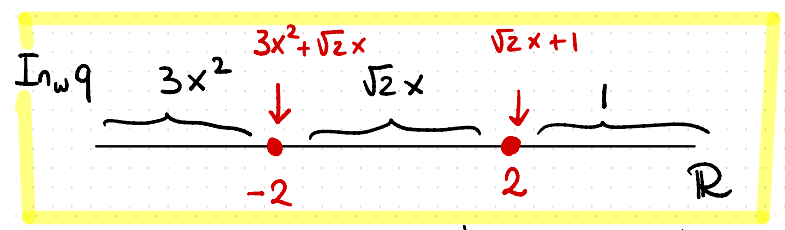
\includegraphics[width=0.5\textwidth]{figs/fig6-3-InitialFormExample.png}
        %\caption{Initial form determination and roots}
        %\label{fig:6.3-InitialFormExample}
    \end{figure}
\end{Ex}

\begin{Th}
Tropical plane curves are balanced, meaning that at every vertex,
$$\sum_{v\in e}w_e\vec p_e=0.$$
Here, $w_e$ is the weight of the edge $\vec p_e$ of the outgoing primitive vector in the direction of $e$.
\end{Th}

Continuing along the lines of the previous example, at the vertex we were examining, we have outgoing primitive vectors 
$$\twobyone{1}{2},\quad\twobyone{-1}{0}\word{and}\twobyone{1}{-2}.$$
Observe that when taking the weighted sum at the vertex, we get 
$$2\twobyone{-1}{0}+\twobyone{1}{2}+\twobyone{1}{-2}=\twobyone{0}{0}.$$
We will prove the theorem next.

\begin{ptcbp}
Any vertex is dual to a face $F_v$ of the Newton polytope subdivision.
For every edge bounding $F_v$, the vector $w_e\vec p_e$ is obtained by the vector tracing the dual edge via a $90^circ$ rotation. We claim to be done due to the fact that the equation being satisfied is equivalent to the fact that the Newton polytope is a closed polygon.
\end{ptcbp}

Imagine that a stick figure with weighted edges comes up to you. We can then check the compatibility condition. If it does not have weights, does there exist an assignment of weights in order to form a tropical curve? 

\subsection{What do the weights mean?}

\begin{Ex}
    Suppose we have a subdivision with edges 
    $$x^2y\to x^5y^2\to x^8y^3\to x^11y^4$$
    and the corresponding edges in the tropical curve. We want to see the initial form. This subdivision \emph{remembers} the monomials that appear in the initial form! It will be a linear combination of the monomials in the edge.
    $$\operatorname{In}_\omega(q)=Ax^2y+Bx^5y^2+Cx^8y^3+Dx^{11}y^4=x^2y(A+Bx^3y+Cx^6y^2+Dx^9y^3)=x^2yP(x^3y).$$
    This polynomial factors so nicely because they lie on the same line! If we are just looking for solutions in $(\bC^\ast)^2$ or asymptotically $|x|,|y|\gg 0,$ the monomial part is irrelevant. Additionally, $\deg(P)$ is equal to the lattice length of the segment. A 1-parameter subgroup orbits $x^3y=r_i$ where the $r_i$ is a root of $P$ counted with multiplicity.    
\end{Ex}




\section{Day 17|20230929}

Last time we talked about edges weighted by lattice length determines the segments of the Newton Polygon it is dual to. Today we will draw topological types of tropical plane curves and cubics. The objective is to experiment with various tropical curves and seek a conjecture to compute their $b_1$. Study a pencil of tropical conics, in other words draw a conic and pick 4 points on it in general position. Then find all conics through those 4 points.

\section{Day 18|20231002}%% TG11




For any interior point of the Newton Polygon, we can make sure that we can find as many cycles can a tropical curve have. There is a correspondence theorem.\par 
The solution to the parameter space of conics is that we get a trivalent tree with $6$ edges. This corresponds to $\bP^5$ which has $6$ boundary divisors.

\subsection{Intersections of tropical curves}

\begin{Def}
    Two tropical curves have a \term{transversal intersection} if they intersect in finitely many points which are not vertices of either curve.
\end{Def}

\begin{Ex}
    Two tropical lines seen as tripods which touch just at a point intersect transversally. 
    \begin{figure}[h!]
        \centering
        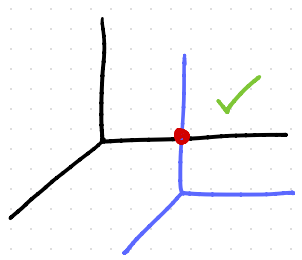
\includegraphics[width=0.5\textwidth]{figs/fig11-1-TransversalIntersectionExample.png}
        \caption{Example of a Transversal Intersection}
        \label{fig:11.1-TransversalIntersectionExample}
    \end{figure}
\end{Ex}

\begin{Ex}
    If the line is placed right on top of the other one, they could also intersect non-transversally on the whole edge.\par 
    If for example we had a conic, it could intersect the vertex of another tropical line non-transversally. Or two vertices could intersect!
    \begin{figure}[h!]
        \centering
        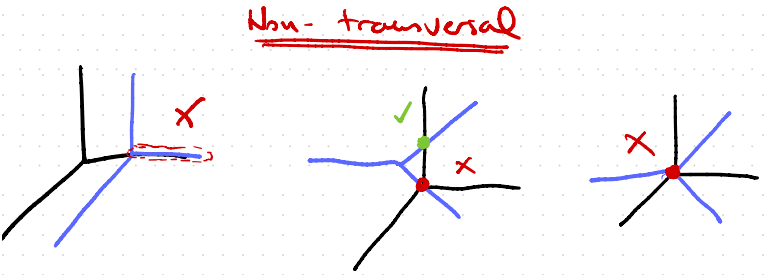
\includegraphics[width=0.8\textwidth]{figs/fig11-2-NonTransversalIntersectionExample.png}
        \caption{Example of Non-Transversal Intersections}
        \label{fig:11.2-NonTransversalIntersectionExample}
    \end{figure}
\end{Ex}

It looks like if the intersection is transversal then the set of intersection is just a point. Otherwise let's be very topological and talk about stable intersections.

\begin{Def}
    For a vector $\vec v\in\bR^2\less\set{0}$, call the \term{vector intersection} of $\Ga_1,\Ga_2$
    $$\Ga_1\cap_{\vec v}\Ga_2=\lim_{t\to 0}\left(\Ga_1\cap(\Ga_2+t\vec v)\right).$$
\end{Def}

\begin{figure}[h!]
    \centering
    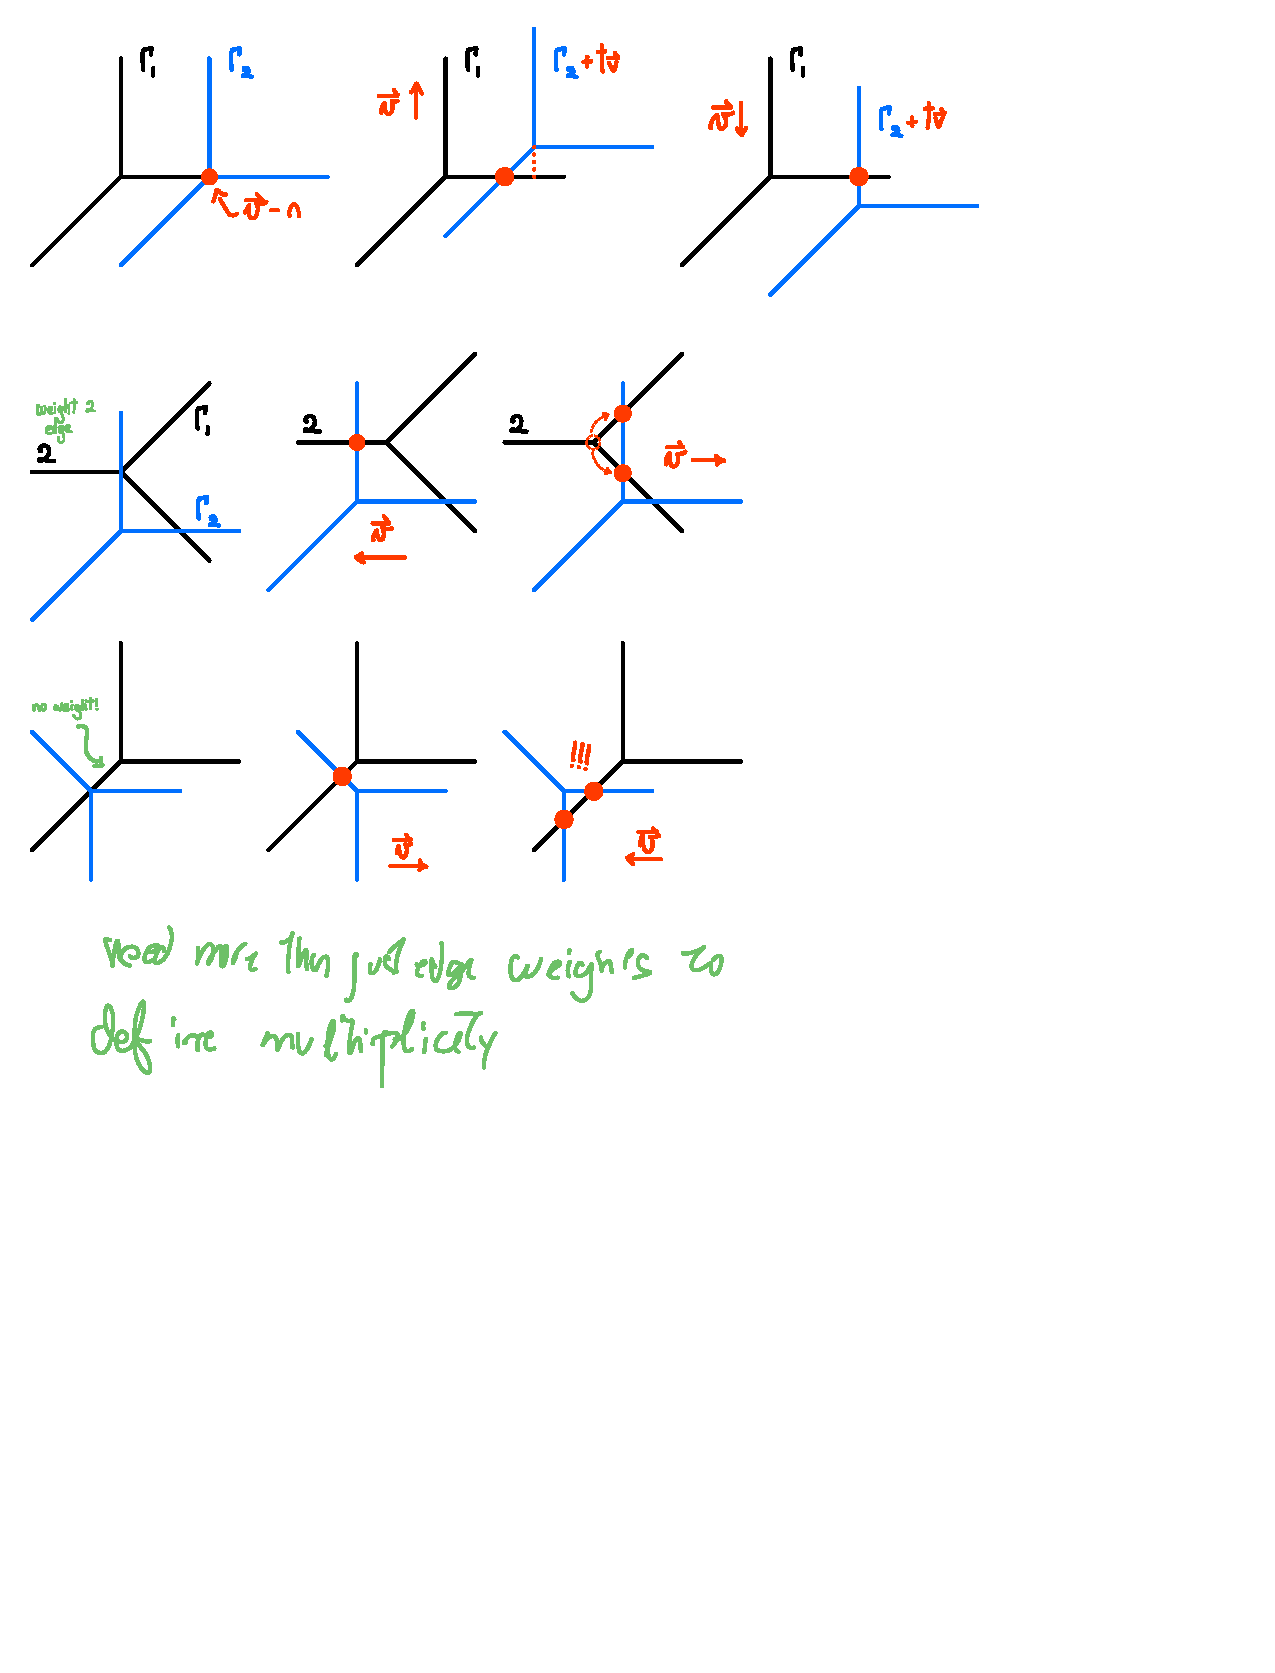
\includegraphics[width=0.8\textwidth, trim= 0.1cm 23.25cm 5cm 0.25cm,clip]{figs/fig11-3-4-and-5-VectorIntersections.pdf}
    \caption{Example of Vector Intersections}
    \label{fig:11.3-VectorIntersection1}
\end{figure} 

Observe that this definition may be troublesome because of the choice of the vector $\vec v$. What happens if we get another intersection point with another $\vec v$?

\begin{figure}[h!]
    \centering
    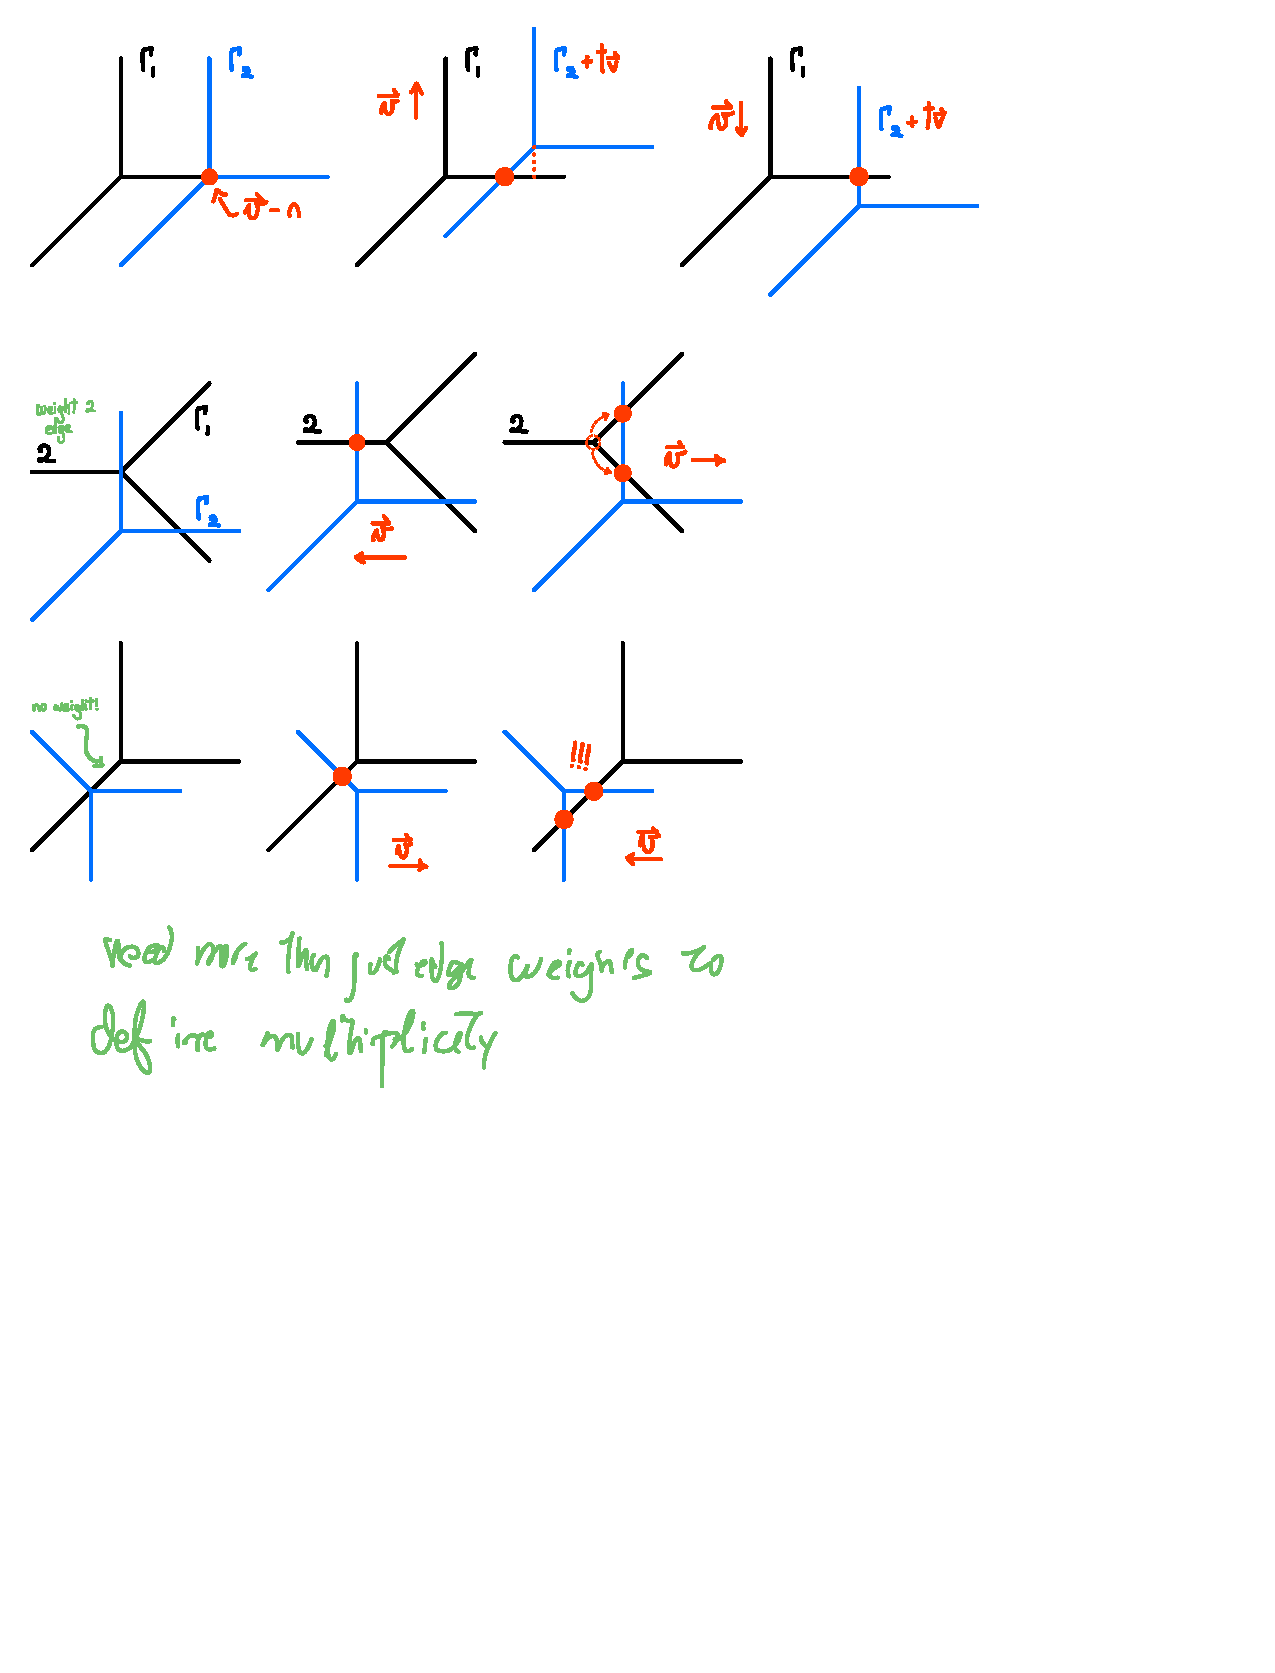
\includegraphics[width=0.8\textwidth, trim= 0.1cm 17.75cm 9cm 5.5cm,clip]{figs/fig11-3-4-and-5-VectorIntersections.pdf}
    \caption{Weighted Vector Intersections}
    \label{fig:11.4-WeightedVectorIntersection2}
\end{figure}
   
From this we deduce that intersection points should be weighted by multiplicity of the edges they belong to. We need more than just the edge weights to define this.

\begin{figure}[h!]
    \centering
    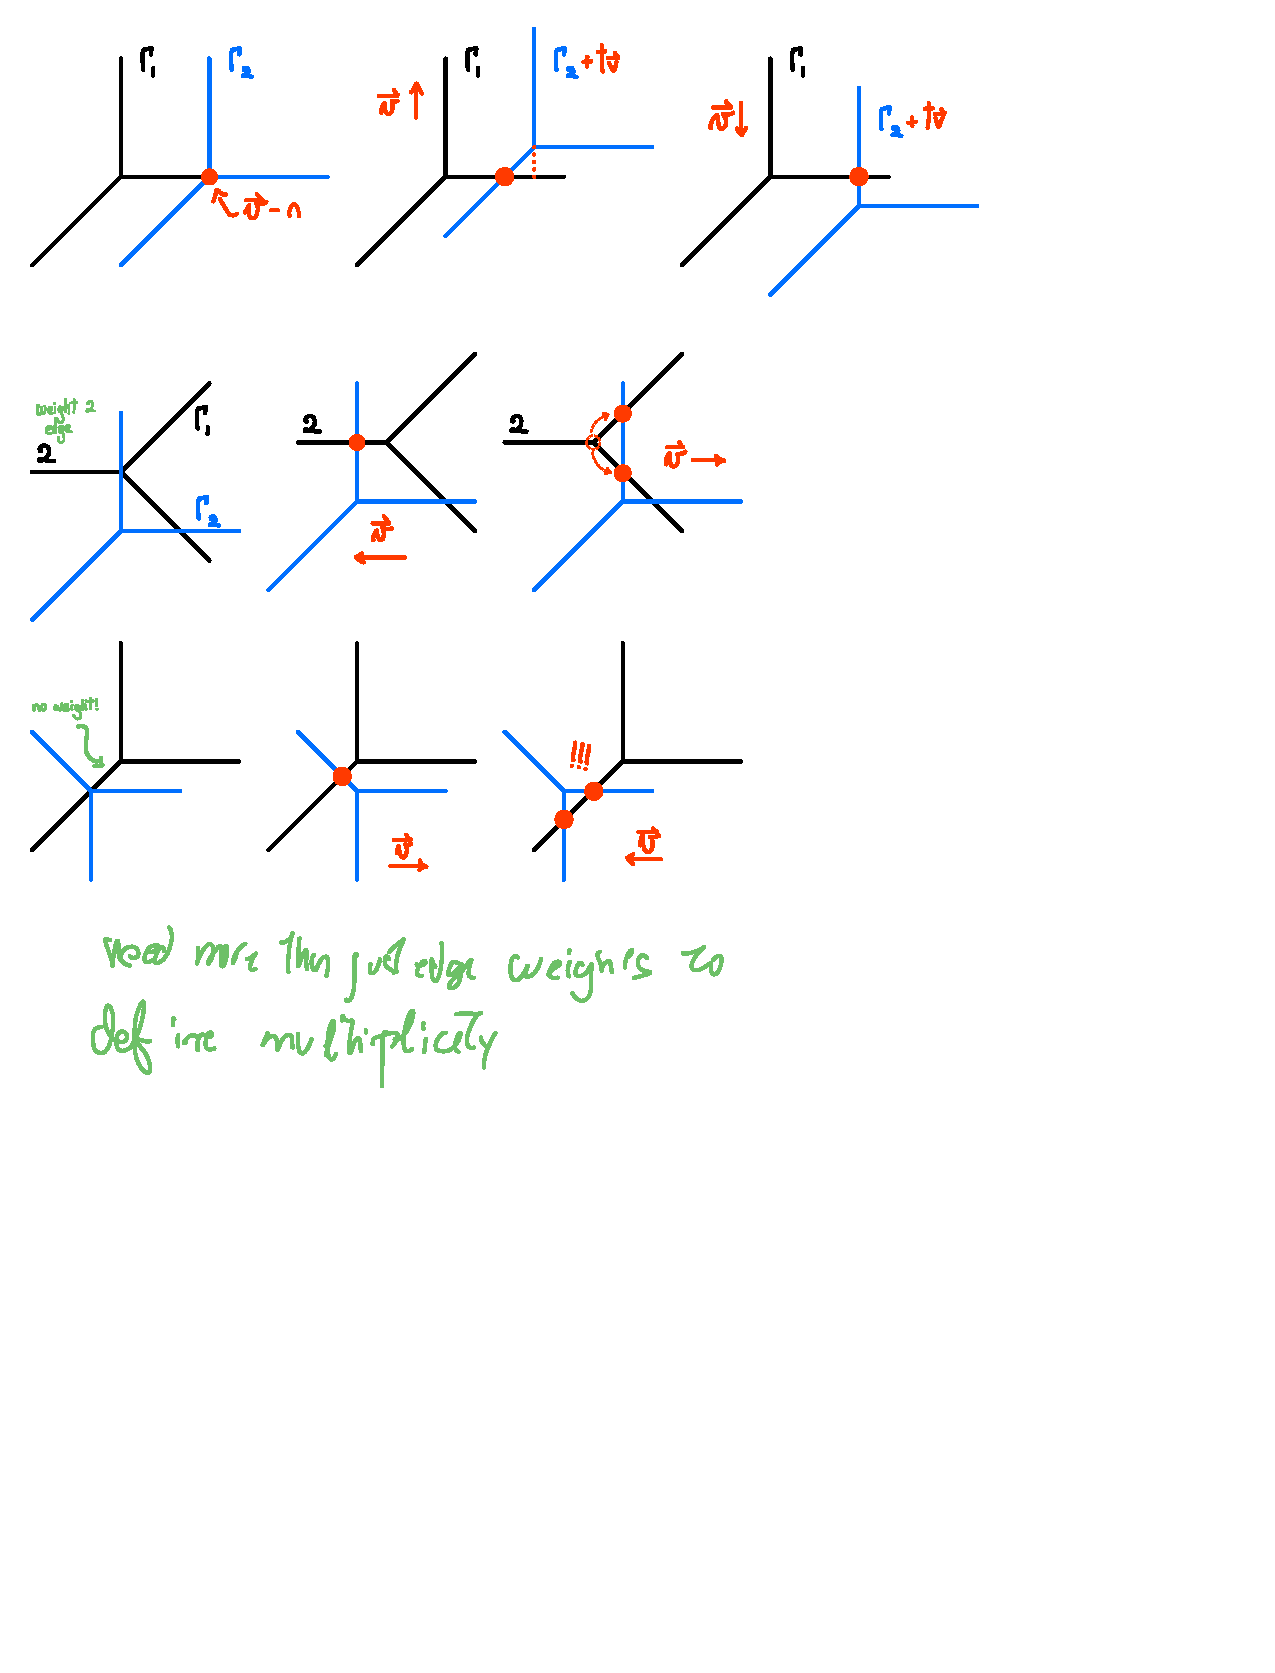
\includegraphics[width=0.8\textwidth, trim= 0.1cm 13cm 9cm 10.75cm,clip]{figs/fig11-3-4-and-5-VectorIntersections.pdf}
    \caption{Problematic Vector Intersections}
    \label{fig:11.5-NonWeightedVectorIntersection2}
\end{figure}
%Amaury Was here
%double checking to see if this worked
Before we jump into the theory, let's have an aside question, let us ask how the curves 
$$C_1=\set{x^a=y^b},\word{and} C_2=\set{x^c=y^d}$$
intersect in $\bC^2$. Observe that we may parametrize $C_1$ as $(x,y)=(t^b,t^a)$ and substitute into $C_2$'s to get 
$$t^{bc}=t^{ad}\To t^{bc}(t^{ad-bc}-1)=0$$ 
which means that at zero we have a point of high multiplicity and $(ad-bc)$ points away from the origin. The interesting question is how does this relate to our problem. At a glance there doesn't seem to be a connection, but if we look at the \emph{valuation} we might just start to see some hints of it.

\begin{Def}
    Let $q$ be a point of transversal intersection of two tropical curves $\Ga_1,\Ga_2$. Then the multiplicity of the intersection is determined by the primitive\footnote{Primitive lattice vectors are the shortest lattice vectors possible}
    directions $\vec p_1,\vec p_2$  of the intersection as 
    $$m_q(\Ga_1,\Ga_2)=w_1w_2|\det(\vec p_1,\vec p_2)|=w_1w_2\bonj{\bZ^2\: \vec p_1\bZ\oplus \vec p_2\bZ}.$$
    The last quantity is the subgroup index of $\vec p_1\bZ\oplus \vec p_2\bZ$ inside $\bZ^2$. %TG11 page 5
\end{Def}
%%https://ocw.mit.edu/courses/12-108-structure-of-earth-materials-fall-2004/9df654250315660f294bf6c9acd49ae1_lec7.pdf PRIMITIVE VECTORS
%% https://en.wikipedia.org/wiki/Unit_cell
%% https://www.physics.rutgers.edu/grad/601/CM601/crystals.pdf




%Amaury Notes begin

\section{Intersection of Tropical Curves}

\begin{define}
Two tropical curves intersect \emph{transversally} if they intersect in finitely many points which are not vertices of either curve.
\end{define}


Our second kind of intersection will be stable intersection.
Let $v \in \RR^2 -\{(0,0)\}$, and define $\Gamma_1 \cap_v \Gamma_2= \lim\limits_{t \rightarrow 0} \Gamma_1 \cap (\Gamma_2 +tv)$, i.e. translate $\Gamma_2$ by the vector $v $. If we were to pick another $v$, our translations would be different. We are forced to ask ourselves if distinct choices of $v$ may lead to different limits.


\begin{note}
    Points of intersections should be weighted by multiplicites of the edged they belong to.
\end{note}



\begin{ex}
    How do the complex curves $C_1=\{x^a=y^b\}$ and $C_2=\{x^c=y^d\}$ intersect in $\CC^2$?

        We can parameterize $x=t^b$, $y=t^a$, then we get $t^{bc}(t^{ad-bc}-1)=0$
\end{ex}


\begin{define}
    Let $p$ be a point of transversal intersection of $\Gamma_1, \Gamma_2$. We let the multiplciity of the point of intersection $p$ to be 
    \begin{align*}
        M_p(\Gamma_1, \Gamma_2):=w_{e_1}w_{e_2} \left| \det \begin{bmatrix}
            P_{1,x} &P_{2,x} \\
            P_{1,y} &P_{2,y}
        \end{bmatrix}  \right| =[\ZZ^2\;|\; p_1 \ZZ + p_2 \ZZ]
    \end{align*}
    Where $p_i$ are the direction vectors of the edges for the interection, $p_{1,x}$ is the $x$ coordinate of the direction vector for edge $1$, and $w_{ei}$ is the weight of the corresponding edge
\end{define}

\section{Day 19|20231004}
%Pages 6 to 8 TG11
Our objective last time was to motivate the idea of intersections with certain multiplicity. With out new definition of multiplicity, does this resolve the issue we had? \red{WHAT WAS THE ISSUE?} The issue is that we must define multiplicity in order to talk about weights/multiplicities of non-transversal intersections.

\begin{Ex}
\red{FIGURE} \blu{WHICH FIGURE THERES NO PICTURE}
In the first case we have intersections at $Q_1,Q_2$, where the first intersection has multiplicity
$$m_{Q_1}=\left|\det\twobytwo{0}{1}{1}{-1}\right|$$
and the other point also has multiplicity $1$. But if we move to the non-transversal intersection we get multiplicity $2$. This goes according to the definition. 
\end{Ex}

\begin{Lem}
The amount of intersections of two tropical curves is invariant under generic translation.
\end{Lem}

The proof follows from two facts:

\begin{itemize}
    \item The definition of multiplicity of an intersection:
    $$m_q(\Ga_1,\Ga_2)=w_1w_2|\det(\vec p_1,\vec p_2)|$$
    \item And the balancing condition at $q$: 
    $$\sum_{e\to v}w_e\vec{p}_e=0$$
    where $e\to v$ means edges incident at $v$.
\end{itemize}

It also suffices to analyze cases locally so we may zoom in into an edge of one of our curves.

\begin{ptcbp}
Consider an edge of a tropical curve $\Ga_1$ locally intersecting $\Ga_2$ at a vertex. The edge of $\Ga_1$ partitions the plane into two half planes $H^+,H^-$.\par 
Let us partition the edges into those ``in'' $H^+$ and $H^-$ and pick $\vec v_+$ in any direction pointing to $H^+$ and let us take the vector intersection with respect to such $\vec v_+$. Considering the multiplicities we get a contribution of 
$$w_1\sum_{e\in H^-}w_e\|\det(\vec p_1,\vec p_e)\|.
\footnote{The edges we have are from $H^-$ because of the relative positions. It does sound counterintuitive however.}$$
Similarly if we take a vector $\vec v_-$ pointing towards $H^-$ and translate $\Ga_2$ in that direction we get a contribution of 
$$w_1\sum_{e\in H^+}w_e\|\det(\vec p_1,\vec p_e)\|.$$
Then the contribution to a $\vec v$ deformed intersection is the same when $\vec v$ points in the direction of $H^+$ or $H^-$.\par 
Suppose $\vec v_1$ and $\vec v_2$ are two vectors pointing in different directions, if we raise the intersection, we get the lower edges intersecting. Their primitive vectors are all in the clockwise direction form $p_e$. So the weight of the $\vec v_1$-deformed intersection is 
           $$\sum_{e'\in E^-}w_ew_{e'}|\det(p_1,p_2)|$$
\end{ptcbp}
%%PAGES 6 to 8 TG11
\subsection{Tropical Bézout}

From this lemma the result follows immediately!

\begin{Th}
Let $\Ga_1,\Ga_2$ be two tropical curves of degree $d_1,d_2$. Then $|\Ga_1\cap\Ga_2|=d_1d_2$.
\end{Th}

A curve has degree $d$ if its dual to a subdivision of $0,(d,0)$ and $(0,d)$. We know that if we have a tropical curve of degree $d_1$ then we can move one of degree $d_2$ in such a way that just so many edges intersect. Counting down we get the product of the multiplicities.

\section{Day 20|20231009}

Last time we started talking about the idea behind Bézout's theorem. Recall, that a curve with degree $d_i$ is dual to the polygon with vertices $0$, $(0,d_i)$ and $(d_i,0)$. Intersections, as in the ordinary case, are counted with multiplicities.\par 
The quantity $|\Ga_1\cap \Ga_2|$ is invariant under translation, so we can move two curves so that only unbounded ends intersect. Looking at this picture from far away and squinting our eyes what we see is two tripods with degree $d_i$. This means that all the information needed to compute the intersection is independent of the subdivisions of the Newton Polygon.
\begin{Def}
    In $\bP^1\x\bP^1$, coordinates are $([x_0:x_1],[y_0:y_1])$, a \term{bi-degree $(a,b)$ curve} is the zero locus of a bi-homogenous polynomial in the aforementioned variables which is 
    \begin{itemize}
        \item homogenous of degree $a$ is $x_i$,
        \item homogenous of degree $b$ is $y_i$.
    \end{itemize}    
    Tropically, this means that $\Ga$ is dual to a subdivision of a rectangle with sides $a$, $b$.
\end{Def}

\begin{Ex}
    The polynomial $x_0y_0+x_1x_0y_1=0$ is a bidegree $(2,1)$ curve. On the tropical side we have \red{FIGURE} which is a $(1,1)$ curve.
\end{Ex}

The tropical Bézout theorem for $\bP^1\x\bP^1$ says that if we have $\Ga_i$ with bidegree $(a_i,b_i)$, then 
$$|\Ga_1\cap\Ga_2|=a_1b_2+a_2b_1.$$

But what if we wanted to intersect a degree $d$ curve with a bidegree $(a,b)$ curve? We just draw the stick figure and notice that degree of the intersection is $d(a+b)$. We can ask how to generalize it and the answer is precisely Bernstien's theorem.

\begin{Th}
Let $\Ga_i$ be tropical curves of degree $\Dl_i$. Then 
$$|\Ga_1\cap\Ga_2|=\operatorname{MixedArea}(\Dl_1,\Dl_2).$$
\end{Th}

In this case the degree of a tropical curve is the Newton polygon of its equation. In other words a lattice polygon.

\subsection{Minkowski Sum of Polytopes}

Once a long time ago we were told that a degree is a number, but a degree is actually a polygon.
\begin{Def}
    Consider $\Dl_i\subseteq\bR^2$ lattice polygon, then the \term{Minkowski sum} is 
    $$\Dl_1+\Dl_2=\set{(x_1,y_1)+(x_2,y_2)\in\bR^2\:\ (x_i,y_i)\in\Dl_i}.$$
\end{Def}
This definition is \textbf{compatible} with translations! At this moment we can choose how to put two polygons in $\bR^2$ and sum them. 

\begin{Ex}
    The Minkowski sum of a square and a right triangle is a gem-shaped pentagon. The idea is that we decide one of the vertices to be the origin and then make the polygon travel through the perimeter of the other one.
\end{Ex}

\begin{Ej}
The Minkowski sum appears to be commutative, prove it! Which other properties does the Minkowski sum enjoy?
\end{Ej}

\begin{Ex}
\red{FIGURE ABOUT MIXED SUDVISIONS}
\end{Ex}

\begin{Def}
    The \term{mixed area} of $\Dl_1,\Dl_2$ is either of 
    \begin{enumerate}[i)]
        \item $A(\Dl_1+\Dl_2)-A(\Dl_1)-A(\Dl_2)$,
        \item the area of the mixed cells in any mixed subdivision of $\Dl_1+\Dl_2$,
        \item the $\la\mu$ coefficient in $A(\la P+\mu Q)$.
    \end{enumerate}
\end{Def}




\chapter{Toric Varieties}
\section{Day 21|20231011}

IT says that if we have two tropical curves of degree $\Dl_1,\Dl_2$ (polytopes), and we wish to compute the intersections, then this is counted via the mixed area. This correspondence is very tight, satisfying. When taking stuff, we get the mixed cells (parallelograms with sides parallel to our original polygons). Having the polygons in positions means that the curves have been moved and the mixed cells correspond to the intersections.\par 
The weight of the edges is the length of sides of the polygon, in particular the Minkowski sum of two lattice polytopes is itself a lattice polytope.

\subsection{Torus actions}

A space $X$ with a torus action $T\.X$ and an open set isomorphic to the torus on which $T$ acts by multiplication is a toric variety. The geometry of a torus is fairly simple or trivial, which means that \emph{most} of the geometry of $X$ can be recovered from the complement of this dense open set (the one isomorphic to $T$). The fact that we have a torus action allows for a \emph{combinatorialization} of the geometric information.\par 
If we don't know what a torus is, it's a group, and the space is just the space. The action moves the points in a certain way. Geometry is connected to the representation theory of the group.

\begin{Def}
    The \term{algebraic torus} of rank $k$ is $G_m^k$ (think of it as $(\bC^\ast)^k$) \aside[If we have a different field than $\bC$, actually $G$ is a multiplicative group \emph{scheme}]. This object is a group under pointwise multiplication and in general we can view it as the scheme 
    $$\Spec\left(\bC\bonj{x_1,\frac{1}{x_1},\dots,x_k,\frac{1}{x_k}}\right).$$
    If we are more familiar with differential geometry, local coordinates are similar but the coordinate is a generalization. We can imagine elements on the scheme as regular functions from the torus to $\bC$. We will usually denote the torus by $T$.
\end{Def}

Recall a group acts on itself via multiplication and in a similar faction the torus action on a space $X$ will be a map $T\x X\to X$. We can thus relate the characters of $T$ to invertible regular functions on $T$ and if we are choosing coordinates, then they are also related to monomial functions in $x_i$'s.\par 
The characters of $T$ are the group homomorphisms from $T$ to $\bC^\ast$. It is actually the trace of an irreducible representation of $T$, but they are one dimensional and\dots Monomial functions on the $x_i$'s are precisely regular functions vanish. Those places are on the coordinate axis so nowhere near the torus. As a $\bC$-vector space, monomials are a basis of our ring. That is gonna play an important role.\par 
All of these interpretations are groups under multiplication. Given a monomial we can read a vector of exponents: 
$$x^3y^{-5}\mapsto (3,-5)$$
so this is also related to the lattice of exponents of the monomial functions. This gives a multiplicative to additive isomorphism. This lattice is called $M$, it is also called the character lattice and is isomorphic to $\bZ^k\subseteq \bR^k$ which we will also called $M_\bR$. This is actually a \emph{tensor product}. In this sense we can match 
$$(3,-5)\mapsto \vf_{(3,-5)}\: T\to\bC^\ast,\ (t_1,t_2)\mapsto t_1^3t_2^{-5}.$$
We also have a relationship between co-characters (linear functions on characters), one parameter subgroups of $T$ (group homomorphisms $\bC^\ast\to T$, $t\mapsto(t^a,t^b))$. The co-character lattice $N$ is the dual of the character lattice is isomorphic to $\bZ^k\subseteq\bR^k=N_\bR$. There is a natural pairing $M\x N\to\bZ$ which turns out to be the usual dot product. Slightly more satisfying, the natural way to get a pairing is to imagine we have a character $\chi$ and a one parameter subgroup $\ga$ we get a map 
$$\bC^\ast\xrightarrow[]{\chi}T\xrightarrow[]{\ga}\bC^\ast,\ t\mapsto(t^a,t^b)\mapsto t^{aA+bB}$$
so the exponent is precisely $\braket{(a,b)}{(A,B)}$.\par
After talking about so many ingredients, let us talk about one more thing. If we have one parameter subgroups, we can think of them as acting on the torus so we have torus orbits. Let's see some torus orbits we get with different actions. 

\begin{Ex}
    Consider the one parameter subgroup $\ga_{(1,1)}(t)=(t,t)$. Acting on a point $(a,b)$ we get the point $(ta,tb)$. So the orbits are lines through the origin. And notice the in fact, $\ga_{(-1,-1)}(t)=(t^{-1},t^{-1})$, even if we get the same orbits, on the first case we get flow inwards while on the second one we get \emph{outwards} flow.\par 
    We could get $\ga_{(1,0)}(t)=(t,1)$, the orbits are horizontal lines. Finally $\ga_{(1,-1)}(t)=(t,t^{-1})$, then the orbits are hyperbolas. 
\end{Ex}

Now we are gonna say ok, we are gonna allow ourselves to grow the torus a little bit by saying that we want to add limit points of one parameter or allow/decide that some monomial functions are regular and some are not and then add the points. In the case of $\ga_{(1,1)}$ we are going to need to fill in the point of the origin. 

\section{Day 22|20231013}

Last time we talked about the setup: the toric variety is a space $X$. One is that it contains the torus as a dense open set and the other is that the torus acts on $X$ and in particular in the open set it acts by multiplication. We linked objects from the algebraic geoemtry and representation theory of the torus. The way we think of characters of the torus are monomial functions on the coordinates of the torus. These are regular functions because there are no poles on the torus. On the other hand $N$ is a lattice of one-parameter subgroups, a map from a one dimensional torus to a $k$-dimensional one. In particular inside the torus, if we take a point and act on it via a one parameter subgroup, we get a one-dimensional orbit. It is always the case that if we let $t=0$ then the point falls off of the torus. These objects are dual to each other via dot product.

\begin{Ex}
    An example of a toric variety is $\bP^1$, the set of homogenous points $[x:y]$. Take out zero and infinity and we get a one-dimensional torus.\par 
    We can also think of points in $\bP^1$ as points of $\bC^\x$ as $[x:1]$ or $[1:y]$. Our objective is to build toric varieties from simpler varieties.
\end{Ex}

\begin{Def}
    A \term{cone} in $N_\bR$ will tell us how to add points to a torus in two ways:
    \begin{enumerate}[i)]
        \item It would tell us what orbits of one-parameter subgroups acquire a limit point when $t\to 0$.
        \item Or it would tell us what monomial functions are regular on such limit points. 
    \end{enumerate}
\end{Def}

Let us illustrate with an example taking two dimensional $N_\bR$:

\begin{Ex}
    A cone is what we think is a cone.\red{FIGURE}
This cone $\sg_1$ contains all lattice points corresponding to one-parameter subgroups of the form 
$$t\mapsto (t^a,t^b),\quad a,b>0$$
Now let's assume that we have a point of the two dimensional torus $P=(r_p,s_p),\ r_p,s_p\neq 0$. We now look at the orbit of $P$ via the coordinate-wise multiplication action:
$$t\.P=(t^ar_p,t^bs_p)$$
and now taking the limit $t\to 0$ of $t\.P$ and we want it to exist, then we introduce three cases:
\begin{itemize}
    \item Both $a,b$ are non-zero.
    \item $a=0$ but $b$ not, then we get points of the form $(r_p,0)$.
    \item The other way around for $b$: $(0,s_p)$.
\end{itemize}
$$\lim_{t\to 0}t\.P=\begin{cases}
    &(0,0),\ a,b\neq0\\
    &(r_p,0),\ a=0\\
    &(0,s_p),\ b=0
\end{cases}$$
The cone contains all the ways to pick the map. All the dots in the \emph{interior} go to zero! If $a,b$ are both zero the action is trivial. This cone is telling us to add the axes to $T$ to get $\bC^2$.\par 
Notice that if we had taken the lower cone we would've obtained a similar situation but instead of adding zeroes we would get infinities. We would still get $\bC^2$ but adding different axes.\par 
If we instead were algebraic geometers we would be interested on regular functions at the limit points. Take $f=x^\al y^\bt$, when is it regular at the $t\to 0$ limit point of the orbit of a 1.p.s. $t\mapsto (t^a,t^b)$, then 
$$f(t)=t^{a\al+b\bt}r_ps_p,$$
the limit exists as long as $a\al+b\bt$ is non-negative. This is precisely the dot product, so we are basically saying that we want all vectors in $M$ whose dot products with vectors in $N$ is non-negative. This defines the notion of \emph{dual cone}. This combinatorial object acquires the meaning of telling us what are the regular functions when adding the limit points. In this case $\sg_1^\lor$ looks exactly like $\sg_1$ \red{PICTURE}. This also tells us that $x,y$ are regular functions so every polynomial in $x,y$ is a regular function. So in particular $\bC[x,y]$ is the ring of regular functions. 
\end{Ex}

Let us focus our attention now on the projective plane.

\begin{Def}
    A \term{fan} is a collection of cones living \emph{nicely} in $N$. This means that we are not just wacking at random at some cones. All cones will have the vertex at the origin and the only overlaps occur at boundary edges. \red{PICTURE}
\end{Def}

This particular fan $\Sg$ is the fan of $\bP^2$. To construct it we follow this strategy 
\begin{enumerate}
    \item Each top dimensional cone produces an affine open chart in the sense of manifolds.
    \item Each face, or ray in common, provides transition functions. 
\end{enumerate}

If we understand how it works in $\bP^2$, generalizing is pretty simple. We will look at dual cones, monomial functions there give us regular functions. 

\begin{Ex}
    The dual to the red cone is itself, the dual to the blue cone is $\set{x<0,0<y<-x}$ and for green its $\set{y<0,0<x<-y}$. Call two monomial functions $x_1,y_1$ on $\text{red}^{\lor}$ so the regular functions are $\bC[x_1,y_1]$.\par 
    On the blue we take the points $(-1,0)$ and $(-1,1)$, they correspond to the functions $\frac{1}{t_1}$ and $\frac{t_2}{t_1}$. But actually let's just call them $x_2,y_2$ so the coordinate ring is $\bC[x_2,y_2]$ so our affine chart is a copy of $\bC^2$ with coordinates $x_2,y_2$. In a similar fashion we will get $\bC[x_3,y_3]$ from the green dual.\par 
    To make them talk to each other, we take a ray in $\Sg$ and ask for its dual. The dual of the positive $y$-axis is the upper half plane. The regular functions for this space are $\bC[\tilde x,\tilde y,\tilde x^{-1}]$ so it is $\bC^\x\x\bC$ with coordinates $\tilde x,\tilde y$. Now notice that this black cone contains the red and blue dual cones. So in particular we can express $x_1,y_1$ in terms of $\tilde x, \tilde y$. The key point is that $\bC^\x\x\bC$ is contained in the two copies of $\bC^2$ we had before. We get the following relations 
    $$\tilde x=x_1=x_2^{-1},\quad \tilde y=y_1=y_2x_2^{-1}.$$
    These are the transition functions which allow us to glue this two patches! 
\end{Ex}

Cones select subsets and produces regular monomials, this produces coordinate ring, take the algebraic variety corresponding to this ring. This variety contains the torus. This can be done in various ways so that's how we build the atlas.

\section{Day 23|20231016}

Then the combinatorial date of the fan gives us a way to construct a toric variety a s a amanigold. Every face gives us the transition functions. The way to construct this chart is the dual cone. Then we take the algebra spanned by the monomials and we ask what variety's coordinate ring is this span. 

\subsection{Consequences of our construction}

\begin{enumerate}
    \item There is an inclusion into closure reversing bijection between cones of $\Sg$ and the torus orbits of $X_\Sg$, the toric variety. And in particular, also exchanging dimension with codimension.\par 
    In action, the fan of $\bP^2$ has 3 two dimensional cones $R,G,B$ and likewise $\bP^2$ has 3 two-codimensional points. Similarly the fan has 3 one dimensional cones. $\bP^2$ has 3 one dimensional torus orbits. From the fan of $\bP^2$ we can immediately read the Euler characteristic of $\bP^2$. The only things that will contribute are the zero dimensional cones.\par 
    In general, to see how the bijection works you can take two different approach:
    \begin{itemize}
        \item The geoemtric approach is: for every cone $\tau$ of $\Sg$, look at the limits as $t\to 0$ of the torus orbits of 1-parameter subgroups $\ga$ with $\ga\in\tau^\circ$. (stuff) and instead we pick a 1 parameter subgroup which lies on a ray, take for example $b=0$, the $y$ coordinate doesn't change and $x$ goes to zero.
        \item The algebraic perspective is that for every affine patch dual to a cone, set all the coordinates that you can set to zero to zero. \par 
        What we mean by that is that if we look at the spec of the algebra dual to  the red cone we get $\bC[x_1,y_1]$ that's why it's affine. Setting both to zero we get the origin. When looking for transition functions, the ray has an affine chart, the algebra generated by the dual cone $\bC[\hat x,\frac{1}{\hat x},\hat y]$. In this case $\hat x$ can't be set to zero. Doing it, we get any non-zero complex number so we get a one dimensional something. And the origin is itself a cone, the dual cone corresponding to the trivial cone is the whole thing. The corresponding algebra is $\bC[x,\frac1x,y,\frac1y]$ and that's why we can't set anything equal to zero.
        \begin{significant}
            Coordinates here correspond to local coordinates in the affine patch. There's a lot of things with the same name. 
        \end{significant}
        Even if in blue we get the same algebra, setting coordinates to zero gives us a different point.
    \end{itemize}
    \item The second useful thing is very natural. $T$-equivarant maps of toric varieties correspond to maps of fans. (Maps of fans: Given $\Sg_k\subseteq N_{k,\bR}$, a \term{map of fans} is a $\bZ$-linear map $L\: N_{1,\bR}\to N_{2,\bR}$ such that for $\tau$ cone of $\Sg$, $L(\tau)\subseteq$ cone of $\Sg_2$.)\par 
    Consider the fan of $\bP^1\x\bP^1$, a 2 dimensional toric variety, for $\Sg,\ X_\Sg=\bP^1\x\bP^1$. We have a projection map $\pi\: X_{\Sg_1}\to\bP^1$ which is equivalent to the map of fans $\tilde{\pi}$ form $\Sg_1$ to $\Sg_2$. It is also the case for $\bP^2\less\set{pt}$ to $\bP^1$ which is projecting from that point.
\end{enumerate}
The proof of this facts is left to the reader. Even without the proof this is a natural statement which makes sense.
\begin{significant}
    $L(\tau)$ doesn't have to be a full cone. In the previous examples it is, but that's just an accident. We would allow it to not be a full cone because we can allow mor maps.
\end{significant}
For example if we wanted to send a line in a plane as a map of.k0

\subsection{Quotient construction}

Given a fan $\Sg$, the toric variety $X_\Sg$ can be obtained as a quotient space of the form:\par 
We start with affine space, cheack the irrelevant locus and then we take something that if we are lucky is a torus:
$$\quot{\bC^N\less\set{irrelevant}}{G}$$
$N$ is the numnber of rays in $\Sg$. The irrelevant set is the set determind by rays that dont span cones.And $G$ is given by lienar relations among maps. 

\begin{Ex}
In $\bP^2$  we have the tripod fan with three coordinates. So we have a $\bC^3$. We throw away the rays which don't span a cone. In this case th irrelevant. This is $\bC^3\less$ \red{FELL ASLEEP}
\end{Ex}


%Amaury notes begin
Last week: Fans $\Sigma$ lead to toric varieties $X_\Sigma$. Maximal cones lead to affine charts, and faces lead to transition functions. $\Sigma \subset N_\RR$. 


we get two neat consequences.
\begin{enumerate}
    \item THere is an incluision into closure reversing bijection between cones of $\sigma$ and the torus orbits of $X_\Sigma$ (also,e xhcanging dimension with co dimension).
    \item $T$-equivariant maps of toric varieties correspond to maps of fans.
\end{enumerate}

\begin{define}
    givne $\Sigma_1 \subset N_{1\RR}$ and $\Sigma_2 \subset N_{2\RR}$ a \emph{map of fans} is a $\ZZ$-linear map $L: N_{1\RR}\rightarrow N_{2\RR}$ such that for every cone $\tau$ of $\Sigma_1$, $L(\tau) \subset $ a cone of $\Sigma_2$
\end{define}
with the embedding, we do not necessarily want to subdivide fans,a s that introduces non trivial orbits.

If a toric varitey is made of toric variteies, torus are homotopic to circles, whch have genus 0, os they contribute trivially.
TO see how this bijection works

\begin{enumerate}
    \item FOr every cone $\tau$ of $\Sigma$, look at the limits a $t \rightarrow 0$ of  torus orbits of $1$-parameter subgroups $|gamma$< with $\gamma \in \tau^0$ (in the interior of the cone $\tau$ ).
    \item For every affine patch dual to a cone, set all the coordinates taht you can set to zero to zero
\end{enumerate}



Toric varieties can be viewed as a genralization fo projective space (we basically have homogenous coordinates). We consider the Quotient Construction. Given a fan $\Sigma$, the toric variety $X_\Sigma$ can be obtianed a a quotient space of the form $\CC^{N}- \{Irrelevalnt\} / G$, where $N$ is the number of rays in the fan $\Sigma$ (for every ray we get a homorgenous coordinate in the toric variety), the irrelevant stuff is the locus determined by sets of rays that do not span cones of the fan, and $G$ is given by linear relations among rays.


\section{Day 24|20231018}

Last time we talked about orbit-cone correspondence for toric varieties. This is a poset-reversing bijection, every biggest cone corresponds to a smallest orbit and vice-versa. In particular, this helps us do really funky things. An orthant corresponds to affine space, the dual cone is the same orthant and those are the coordinates of affine space. The fan with only the axes is $\bC^2\less\set{(0,0)}$ and so on.\par 
Maps of fans corresponds to good maps of toric varieties. They both have combinatorial descriptions, maps beteween fans are the restriciton of an integral linear map between vector spaces. Cones of the first fan move to cones of the second fan. Integral in the sense that integer coefficients.\par 
With that now we have a quotient construction: take $\bC^N$ remove \emph{stuff} which is obtained from equations coming from rays that do not span a cone and then we mod out by linear relations among rays.

\begin{Ex}
    In the case of $\bP^2$ we have the fan which looks like a tripod. As it has $3$ rays we begin with $\bC^3$. Each ray corresponds to a coordinate of $\bC^3$: $x,y$ and $z$. The only subset of rays that does not span a cone of the fan is the three rays together $\set{\rho_x,\rho_y,\rho_z}$. We take the coordinates corresponding to the rays and set them equal to zero. Then we take that locus and throw it away: $\set{x=y=z=0}$. The way to determine the group is that we see the primitive vectors: $\vec p_x=\vec 1,\dots$ $p_z=-e_1-e_2$ and the fact that we have one relation 
    $$1\.p_x+1\.p_y+1\.p_z=0$$
    means that the torus is one dimensional. $t$ acts on $(x,y,z)$ as $(t^1x,t^1y,t^1z)$. The quotient we obtain is 
    $$\quot{\bC^3\less 0}{\bC^\x}.$$
    Observe that the exponents in the action are the coefficients in the relation.
\end{Ex}

\begin{significant}
If the coefficients were $2,3,4$ the action would be $(t^2x,\dots)$
\end{significant}

If we were working with $\bP^1\x\bP^1$ the quotient would be by $(\bC^\x)^2$ and the action would be $(s,t)\.(x_1,x_2,y_1,y_2)=(sx_1,sx_2,ty_1,ty_2)$. More relations means more copies of $\bC^\x$. The real question is \emph{why is this true}? What if we take a fan and declare that any ray of the fan becomes a basis of a new vector space? Artificially we create a vector space.

\begin{Ex}
    In the case of the $\bP^2$ fan, $\vec p_x$ becomes $(1,0,0)$ and so on. Now we want to lift the other cones as cones generated by the vectors. The space we just made is the first quadrant. All the cones that we get are in the totally positive quadrant. We are actually missing a three dimensional cone. We have \emph{removed} from this fan that 3-cone. The orbits we are removing are \emph{not} lifts of cones back in the tripod. Now what we want is a map of fans that will make the quadrant go into the tripod. This will be a map of vector spaces. In particular in this case the map is projection by $(1,1,1)$. This is a one-parameter subgroup of the torus. Basically the orbits of our one-parameter subgroup get identified, so the projection is the quotient map of the action whose exponent vector is the coefficients of the relation.
\end{Ex}

\subsection{Tropicalizing Toric}

In tropical geometry, the \emph{field} is the tropical numbers $\bR\cup\set{\infty}$, then $k^\x$ is $\bR$. So the torus which is $(k^\x)^n$ is $\bR^n$, since multiplication is the action, then tropical multiplication corresponds to addition. 

\begin{Ex}
    How do we make the tropical projective plane $\bP^2$? Remember we had the fan of $\bP^2$ (the tripod inside $N$) and then from here we got the dual cones inside $M$. Each of the dual cones gave us a copy of $\bC^2$ and then we had transtition functions of the form $x_2=\frac{1}{x_1}$, and $y_2=\frac{y_1}{x_1}$. Also between red and green $x_3=\frac{x_1}{y_1}$ and $y_3=\frac{1}{y_1}$. This is what we did a couple of days ago.\par 
    To do it tropically we do it exactly the same, but instead of $\bC^2$ we get $\bT^2$. Specifically three copies with coordinates:
    $$\bT^2,x_1,y_1,\quad\bT^2,x_2,y_2,\quad\bT^2,x_3,y_3.$$ 
    These sets are basically copies of $\bR^2$ with lines at infinity so we get points like $(\infty,\infty)$, $(\infty,r)$ and $(s,\infty)$. Now we have to glue this things together to obtain one space. Every time we see a times we see a plus actually:
    $$x_2=-x_1,\quad y_2=y_1-x_1,\quad x_3=x_1-y_1,\quad y_3=-y_1$$
    To see what this objects glue to, take for example the line $(s,\infty)$, in the second $\bT^2$ we get $x_2=-s$ and $y_2=\infty-s=\infty$ (this is ordinary algebra). So the $(s,\infty)$ line maps to line at infinity \emph{in the reverse direction}. For the $1\to3$ transitions we get $x_3=s-\infty=-\infty$ and $y_3=-\infty$.\red{Finish discussing}.\par 
    What happens is that we get an infinite triangle.
\end{Ex}


%----------Amaury after this


Toric varieties have an orbit cone corespondence. THis a bijection between the cones of a toric variety, and the toric orbits.  We have that good maps of toric varieties correpsond to maps of fans. We also hav a quotient contruction $X_\Sigma = \CC^N - \{stuff\}$, where $N$ is the number of rays, the stuff is the collection of rays not spanning a cone, and $G$ is a linear relation among rays.

\begin{ex}
    $\PP^2$ has three rays, denoted by $P_Y$, $P_X$, and $P_Z$. THe only subset of rays NOT spanning a cone is the subset $\{P_X, P_Y, P_Z\}$ (any two span a cone). so we throw away the locus $\{X=Y=Z=0\}$, i.e.e the origin. The relation we have between the three is that $1P_X + 1 P_Y + 1 P_Z=0$ (the vectors are $P_X=(1,0)$, $P_Y=(0,1)$, and $P_Z=(-1,-1)$). all of the 1's tell us we have a one dimensiaonl torus, and our action will be $t(X,Y,Z) = (t^1 X,t^1,Y,t^1Z)$ With these relations, we get $\CC^*$

    Now,w e can take the fan, and declare that any ray of the fan is generated bya  basis vector of a new vector space. so $P_X=(1,0,0)$, $P_Y=(0,1,0)$, and $P_Z=(0,0,1)$. Then our three corrsponding rays in $\RR^2$ become the three positive half lines of the X, Y, Z axis. Now we want to lift the cones in our toric variety, so we get octant planes Now, everything we make is contained in the first octant of $|RR^3$, so ths is a subset of all the cones of the first octant, but the first octant with removal Bu the first octant is $\CC^n$, and we removed something. We remove orbits corresponding to not being centered in th eoctan, i.e.e we remove the three dimensional cone, so teh toric variety is $\CC^3$ minus the orbit correpsonding to the cetner cone, whcih is $(0,0,0)$.
\end{ex}





In tropica geoemtry, $k $ is identitfied with $\TT= \RR \cup \{\infty\}$, then $k^*$ corresponds to $\RR$> THen $T= (k^*)^n$ correpsonds to $\RR^n$, and the action $*$ corresponds to $+$. 



How to make tropical $\PP^2$




\section{Day 25|20231020}

Patching construction for toric varieties: Dual cone gives affine patches, edges give transtition functions. This can be switched to tropical numbers. The charts are now affine $\bT$ spaces, sometimes it could be without infinity. Transition functions become linear.\par 
With the example of $\bT\bP^2$ we had an infinite triangle. By removing the line and two points all we get is a copy of $\bT^2$. The $y$-axis of the first chart sticks to the $y$-axis of the second chart, while the $x$ axis becomes $y=x$. \red{LOOK AT PICTURE}
\begin{Rmk}
When removing the lines at infinity we get a copy of $\bR^2$, which is just the tropical torus! Even if the lines are arranged differently, the charts differ by an element of $\GL(\bZ)$. 
\end{Rmk}

The difficulty of transforming this into a general process is just painful notation. This process can always be done.

\begin{itemize}
    \item The tropical toric variety $\bT X_\Sg$ has a \emph{stratification} into $\bR^k$ strata which has a natural poset isomorphism with the stratification of the toric variety of $X_\Sg$.\par 
    \red{AUDIO AROUND 10min} Stratification means a disjoint union into locally closed spaces. Think of it as chopping into pieces of different dimensions. All pieces are tropical tori $\bR^k$ for some $k$. 
    \item The tropical toric variety has the structure of an ``infinite polytope'' (not precise, but it's what me imagine) which the normal polytope or dual to the fan of the toric variety.\par 
    In the case of $\bP^2$, the fan is the tripod fan. For every 0-cell, we have a 2-stratum, for every ray we have a codimension 1 stratum whihc is incident at exactly one point. And for each 2-cone we have a 0-strata. This is similar to the orbit-cone correspondence, now its a dimension reversing map. Composing both we get a dimension-\emph{preserving} map. \blu{AUDIO BEFORE 17 min}\par 
    The role taken by limits as $t\to 0$ of $t\.p$ in complex toric land, is replaced by $\lim_{T\to\infty}T+P$. In particular, given a 1-parameter subgroup $(1,1)$, what are the orbits?\par 
    They will act on a point $(x_1,y_1)$ as 
    $$T\.(x_1,y_1)=(x_1+T,y_1+T).$$
    With this, no matter where we start, we go to $(\infty,\infty)$. The cones of the toric variety tells us how to add the point to infinity, it works the same way here but the action is now additive instead of multiplicative. 
\end{itemize}

\subsection{The Quotient Construction}

Let's go back to $\bP^1$. In our quotient construction this is 
$$\bP^1=\quot{\bC^2\less\set{(0,0)}}{\bC^\x},\quad t\.(x,y)=(tx,ty).$$
We now read the same information from the fan, our affine space is over tropical numbers now:
$$\bT\bP^1=\quot{\bT^2\less\set{(\infty,\infty)}}{\bR},\quad T\.(x,y)=(T+x,T+y).$$
Without considering anything as of now, just by intuition, the tropical projective line should be a line segment! Formally when constructing like this, we first remove the point at infinity and then look at the orbits. They are all parallel lines and each correspond to one point in the quotient. \red{PICTURE 32min}

\subsection{Subvarieties}

We aim to answer the question about how subvarieties behave under tropicalization. The main point is that we begin with a curve in a torus and then we tropicalize.\par 
Suppose now $Y\subseteq T\subseteq X_\Sg$, where $T$ is a torus and the other is a toric variety. What is 
$$\Trop(Y)\subseteq\bR^n\subseteq \bT X_\Sg?$$

\begin{Def}
    The \term{extended tropicalization} of $Y$ inside $X_\Sg$ is the closure of $\Trop Y$ inside $\bT X_\Sg$. 
\end{Def}

\begin{Ex}
    Lines in $\bP^2$ give rise to tropical lines (tripods) in $\bR^2$. Now we know that we can close this as tropical $\bP^2$. Then we take the closure in $\bT\bP^2$ so we only get 3 additional points. \red{PIC 41 min}
\end{Ex}

\begin{Ex}
    Same line as before but we close in $\bP^1\x\bP^1$. So now we compactify inside an infinite square. Before the 3 points were part of 3 one dimensional orbits, but now one of the points corresponds to a zero-dimensional stratum.
\end{Ex}

\begin{Ex}
    If we let a line go through the origin and close in $\bP^2$. The corner locus is $\min(x,y)$ which is non linear where $y=x$. Closing in $\bP^2$ gives us a point in a line and a point in the point. But when closing in $\bP^1\x\bP^1$ we get only points.
\end{Ex}

We wish to discuss how the position is related to the original position of the complex variety.

%------- Amaury after this


\section{Tropical Toric Varieties}

From th efan $\Sigma$ we use tropical numbers and tropical operations for transition functions, i.e. $\TT \PP^2$ provides us with $\TT^2, x_1,y_i$, for $i=1,2,3$. We get relations from $i=1$ and $i=2$ via $x_i=-x_2$ \& $y_1=y_2-x_2$, from $2$ to $3$ via $x_2 = y_3-x_3$ \& $y_2 = -x_3$, and finally from 1 and 3 via $x_1 = x_3-y_3$ \& $y_1 = -y_3$.

We get invertible in GLZ, which is our notion of automorphism of the torus. We can always do this translation. We observe that the tropical toric variety $\TT X_\Sigma$ has a stratification into ``$\RR^k$''strata, whcih has a natural poset isomorphism with the stratification of the complex toric variety toric variety $X_\Sigma$. 
Furthermore, $\TT X_\Sigma$ has the structure of an $``\infty''$ polytope, i.e. scale the polytope so that lengths go to infinity, which is the normal/dual polytope to the fan of $X_\Sigma$.

A stratification is a disjoint union into locally closed spaces. We get 0-dim, 1-dim, and 2-dim spaces, each is a tropical tori. THis is similar as how $\CC\PP^2$ has a startification as points, lines, and the surface of the triangle. 



Now, the shortcut to get the tropical troic variety via the fan of $\PP^2$, we make rays orthogonal to the rays of $\PP^2$, introduce fans correspodnign to each of the 2-dim pieces of the fan, and set the lines to infinty.

The role taken by $\lim\limits-{t\rightarrow 0} t*p$ in $\CC$-toric land is replaced by $\lim\limits-{T \rightarrow \infty} T+p$ in tropical rotic land. So if we tak e a one parameter subgroup, say $(1,1)$, and we ask for hte orbits of this subgroup, the orbits are found fvia $T(x_1,y_1) = (T+x_1,T+y_1)$. SO regardles of the starting point, the orbit gets to the point at infinity. FOr the one parameter subgroup $(2,1)$, we have $T(x_1,y_1) = (2T+x_1, T+y_1)$.



We can also show how the quotient construction works tropically. We being at $\PP^1$. IN our quptient construction, this is $\CC^2-(0,0)/\CC^*(t(x,y)=(tx,ty))$, where $t*(x,y)=(tx,ty)$. THe one parameter subgroup comes from the linear relation on the fans of $\PP^1$, the relation being $p_1+p_2=0$. Now we do the same from the fan to get us into tropical space. $\TT\PP^1 = \TT^2 -(\infty, \infty)/\RR (T(X,Y)=(T+X,T+Y))$, where $\RR$ is the torus on $\TT$. We expect $\TT\PP^1$ to be a line segment, as we have $\PP^1$ is two rays connected. We get a point for the first ray, a point for the second, and a line connecting the two. THis is related to initial forms (See other texts).


We have parallel lines connecting to the singular point at infinity which we remove. This means that each parallel ray hits a different point at infinity. We can create an orthoognal line to these rays, and we say this ray hits two other points at infinity (at the limtis of identifying the x and y axis).



We get some kind of orthogonal line to these parallel rays, and this line intersects each orbit exactly once. This line connects at poitns which represent $(\infty,0)$ and $(0, \infty)$. 


We have our original consturction of tropical curves. Now, assume we have $Y \subset Torus \subset X_\Sigma$, so a curve in a torus in a toric variety. Now e have $Trop(Y) \subset \RR^n \subset \TT X_\Sigma$. 

\begin{define}
    The \emph{extended Tropicalization} of $Y$ inside of $X_\Sigma$ is the closure of $Trop(Y)$ inside of $\TT X_\Sigma$.
\end{define}


So we start with a line $L \subset (\CC^*)^2 \subset \PP^2$. This gives rise to a tropical line $Trop(L) \subset \RR^2$. THe closure of $Trop(L)$ gives three aditional points, one for each section of the tropical $L$ which hits lines at infinities. 


Next time, we will compare the combinatorics of troical liens in varieiteis to toric varieities. 



\section{Day 26|20231023}

Recall we defined the tropicalization of a toric variety and if we had a $Y\subseteq T\subseteq X_\Sg$ then the tropicalization in $X_\Sg$ is 
$$\ov{\Trop(Y)}\subseteq \bT X_\Sg.$$
\begin{Ex}
    By taking the equations $x+y+1=0$ and $y+1=0$ then the associated tropical lines are a tripod and a horizontal line. We may either embed them into $\bP^2$ or $\bP^1\x\bP^1$.\par 
    We know that tropical $\bP^2$ looks like an infinite triangle while the other looks like an infinite square.\red{FIGURE around 5 min}
\end{Ex}

What will discuss is the relation between how the clousure of $Y$ in $X_\Sg$ intersects the orbits with respect to the intersections of the tropical toric variety. We summarize this into a question 

\begin{significant}
    Given $Y\subseteq T\subseteq X_\Sg$
\end{significant}

In the first example, $x+y+1=0$ is a line which closed into $\bP^2$ intersects 3 lines in $\bP^2$. In tropical land, it intersects the 3 copies of $\bR$ and misses the vertices. While in $\bP^1\x\bP^1$, the correspondence persists. The fan of $\bP^1\x\bP^1$ consists of 4 rays and 4 2 dimensional fans. In this case one of the edges of the tripods is inside the 2 dimensional fan which is dual to the vertex that \red{Didn't understand}

\begin{Th}
Assume $K$ has a trivial valuation and $\sg\in\Sg$ a cone. Then 
$$\ov Y\cap O_\sg\neq\emptyset\iff \Trop(Y)\cap\sg^\circ\neq\emptyset.$$
\end{Th}

\begin{Rmk}
Trivial valuation implies that when \emph{throwing the blanket}, everything stays at the same level.
\end{Rmk}

\begin{ptcbp}
To show the result, we will show that both facts are equivalent to the statement. \red{SLEEP} Put yourself in a local chart that contains this orbit. This is a copy of $\bC$.\red{sleep}\par 
Now we want to show that a face intersection then the non-extended intersects the interior of the cone. This is because the tropical toric variety is dual to the fan. The trivial valuation gives us a tropicalization which is always a cone over the origin. 
\end{ptcbp}

In conclusion, we know that if we draw a tropical curve which corresponds to an algebraic curve in the torus, after closing it into the toric variety we will know which orbits we intersect just by looking at the variety.\par 
If we are an algebraic variety $Y$ inside a torus, which toric variety do we want to be compactified into? The answer lies in the tropicalization.\par 
But what does this question even mean? 
\begin{itemize}
    \item The variety $Y$ certainly wants to be compact.
    \item It also doesn't want to acquire a whole bunch of singularities. (Think about the Alexandroff compactification, one-point compactification. Good luck doing geometry there.)
    \item To compactify we must add some points, and since we are in a \emph{stratified} toric variety, the stratification of $\ov Y$ inside $X_\Sg$ matches, including dimension grading, with the stratification of $\Sg$. 
    \item Lastly the compactification must not bw wasteful (because varieties care about the enviroment). The torus itself shouldn't have so many points not needed to compactify.
\end{itemize}
$x+y+1=0$ likes to be compactified in $\bP^2$ as \red{picure}. Except none of the infinite points are touched, so it likes to be compactification in $\bP^2$ without the three infinite points. \red{picture}.




\section{Day 27|20231025}

Last time we had a subvariety of a torus which is the open dense set of a toric variety. The question we addressed was 
\begin{significant}
    What are the orbits of the toric variety that $\ov Y$ intersects?
\end{significant}mn,
An orbit intersects the closure of $Y$ iff the tropicalization of $Y$ intersects the relative interior of the cone corresponding to the orbit. This went through an intermediate step, extended tropicalization intersects the face corresponding to $\sg$. Now we know when an orbit intersects $\ov Y$.\par 
Stepping up sophistification, if we have a $Y\subseteq T$, when is the toric variety a good choice to close $Y$ in? 
\begin{itemize}
    \item When $\ov Y$ is compact/complete. (Not synonyms, compact in Zariski is trivial but Euclid not. Complete means all limit points.)
    \item When $\ov Y$ doesn't become too singular
    \item When codimension $i$ strata of $\ov Y$ corresponds to codimension $i$ \emph{stuff} of $X_\Sg$ 
\end{itemize}
We can always take a toric variety corresponding to a complete fan which corresponds to a compact toric variety so that's where we wanna close $Y$ into.\par
Recall we saw the example $x+y+1=0$ inside the torus $(\bC^\x)^2$ then we can close it into $\ov L\subseteq \bP^2\less\set{e_1,e_2,e_3}$. And looking at the tropicalization of $L$, it happens to be the fan of $\bP^2\less\set{e_1,\dots e_3}$. We ask now, why is this not a coincidence?\par 
In what follows, $K$ is trivially valued. Any Newton Polygon will not be subdivided.

\begin{Th}
$Y\subseteq T_n$ is $d$-dimensional and irreducible and $\ov Y\subseteq X_\Sg$ the closure of $Y$ in $X_\Sg$ then 
$$\ov Y\word{is complete}\iff \Trop Y\subseteq |\Sg|.$$
\end{Th}

The support $|\Sg|$ is the locus of points in $N$ that belong to some cone of $\Sg$.

\begin{ptcbp}
Assume by contradiction that $\Trop Y$ is not inside of $|\Sg|$. Let us draw a picture: \red{figure 20 min}
So let us add fans to get a complete toric variety. Consider a complete fan $\tilde \Sg$ that contains $\Sg$ as a sub fan. In the picture $\tilde \Sg$ is both red and green. Complete means that the support is the whole vector space. Then by a known theorem $X_{\tilde{\Sg}}$ is compact and also has $X_\Sg$.\par 
Their difference is $\bigcup_{\sg green}O_\sg$ by the orbit cone correspondence something.\par 
Because $\Trop Y$ intersects the green cone, then the closure has a point in the orbit corresponding to the green cone. That means $Y$ has a limit point in the cone corresponding to the differnece. So when closing in $X_\Sg$ that point\dots\par 
As $\Trop Y\cap \sg^\circ\neq\emptyset$, for some green cone $\sg$, then $\ov Y\cap O_\sg\neq \emptyset$. Say $y$ is a point in such intersection, $y$ is a limit point of $Y$ in $X_{\tilde\Sg}\less X_\Sg$. So this means that $\ov Y\subseteq X_\Sg$ is not complete.\par 
Let's go the other direction now, assume $\Trop Y\subseteq |\Sg|$. We add cones to $\Sg$ to get a complete fan $\tilde \Sg$:
$$Y\subseteq T\subseteq X_\Sg\subseteq X_{\tilde \Sg} (\text{compact}).$$
Lets draw another picture (\red{fig 30 min}), when closing $Y$ inside $X_{\tilde\Sg}$ we get a compact \red{sleeping} But $\ov Y\cap O_\sg$ is empty for all orbits in $X_{\tilde{\Sg}}.$
\end{ptcbp}
\red{SLEEP SLEEP}
\begin{Th}

\end{Th}

\begin{ptcbp}
For tevery $\sg$, $\ov Y\cap O_\sg\neq \emptyset$ and $\dim(\ov Y\cap O_\sg)=d-dim\sg$ iff $\Trop Y=|\Sg|$.\par 
We must show $|\Sg|\subseteq\Trop Y$
\begin{enumerate}
    \item Every cone in $\Sg$ must intersect $\Trop Y$, in other words $\sg^\circ\cap\Trop Y\neq\emptyset$.
    \item The cones of $\Sg$ are at most dimension $d$. Which comes from the hypothesis. If $\Sg$ had a $d+1$ dimensional cone, this corresponds to an orbit of codimension $d+1$. By the first observation it should intersect $\ov Y$, but that means 
    $$\dim (\ov Y\cap O_\sg)=d-(d+1)<0\To \ov Y\cap O_\sg=\emptyset$$
    which contradicts our first observation.
    \item If we have a $d$-dim cone of $\Sg$ its not possible to be intersected by $\Trop\Sg$ in a smaller dimension. This means $\Sg$ has cones of higher dimension.
    \item Is it possible to be covered by higher dimensional? Not possible because balancing condition.
\end{enumerate}
\end{ptcbp}






\section{Day 28|20231027}

The big picture is that our world has trivially valued field and we have a subvariety of a toric variety. We looked at the combinatorial properties of tropicalization, what we should hold is that tropical toric varieties are like adding stuff to a torus which corresponds to cones in a space. We concluded that if a tropicalization is contained in the support of a fan then the variety is compact. The last property we wish to prove is dimension transversality. Those properties are equivalent to the fact the the tropicalization \emph{is} the support of the fan.

\begin{ptcbp}
We already know that $\Trop(Y)\subseteq |\Sg|$, we want to show the other inclusion. 
\begin{enumerate}
    \item Every cone $\sg$ in $\Sg$ must intersect $\Trop Y$. If we have a cone that doesn't intersect $\Trop Y$, we should throw it away.
    \item The dimension of $\Sg$ as a fan is \emph{at most} the dimension of $Y$. This is because we assumed 
    $$\codim_{\ov Y}(\ov Y\cap O_\sg)=\codim_{X_\Sg} O_\sg.$$
    \item If we have a top-dimensional cone of $\Sg$, then it can't intersect $\Trop Y$ in a positive codimensional locus. Otherwise $\Trop Y$ would intersect $d+1$-dimensional cones of $\Sg$ (which don't exist).\red{pic 10 min}
    \item A top dimensional cone of $\Sg$ cannot be partially covered by $\Trop Y$. This would violate the balancing condition for $\Trop Y$. What does it mean to be balanced along $\tau$? We go to the quotient by projecting down. We quotient away the linear span of $\tau$. So the cones now become $1$-dimensional and so we can apply the old definition of balancing.\par 
    If that were to be the case, now we take $\tau$ a face of $\Trop Y$, then the point is unbalanced. 
\end{enumerate}
Altogether, every $d$-dimensional cone of $\Sg$, must be completely covered by $\Trop Y$ then $|\Sg|\subseteq\Trop Y$. \blu{Renzo is thinking very hard about the drawing around 25min} Apparently the last comment is not true. When checking incidence conditions, we only care about cones incident to a face.\par 
For the other direction we want to show the properties. We need the following facts:
\begin{enumerate}
    \item There are no positive dimensional compact subvarieties of tori. Tori are full of holes. Prove it for $\bC^\x$ and then induction.
    \item An orbit of codimension $k$ of a toric variety is locally a complete intersection.
    \item For any $Z\subseteq X_\Sg$ and a hypersurface, the intersection with $Z$ either remains the same dimension or the dimension goes down by 1 or they have empty intersection.
\end{enumerate}
With this we tackle the other side of the theorem. Take a top dimensional cone $\sg_d$ in $\Sg$. Then $O_{\sg_d}$ is a codimension $d$ orbit and $O_{\sg_d}$ intersects $\ov Y$ non-trivially. We know $O_{\sg_d}$ is isomorphic to a torus and because $\ov Y$ is complete, then $ O_{\sg_d}\cap\ov Y$ is complete and so it has a finite number of points. \red{LAST PICTURE} At every step we have to drop codimension by one.
\end{ptcbp}

When all of the conditions happen, we may have a new concept!

\begin{Def}
    $\ov Y\subseteq T\subseteq X_\Sg$ is a \term{tropical compactification} when $\Trop Y=|\Sg|$. In particular the properties of the previous theorem hold.
\end{Def}

Right now we haven't talked about how singular $Y$ become when compactified. Let us just talk a bit. A tropical compactification.

%------Amaury after this


\begin{theorem}
    $\overline{Y} \cap O_\sigma \neq \emptyset$ and dimensional transversality $codim_{\overline{Y}}(\overline{Y} \cap O_\sigma) = codim_{X_\Sigma}(O_\sigma)$ iff $Trop Y= |\Sigma|$
\end{theorem}

\begin{proof}
   $\implies$ we know that $trop(Y) \subset |\Sigma|$. We want to prove $\supset$. First, we have that any $\sigma \in \Sigma$ must intersect $trop Y$, as $\overline{Y} \cap O_\sigma \neq \emptyset$. Second, we have that $\dim(\Sigma)$ is at most $\dim(Y)$, by the dimensional transversality. Third, we have that a top dimensional cone of $\Sigma$ cannot intersect $trop(Y)$ in a positive codimension locus, otherwise $Trop(Y)$ would intersect $(d+1)$ dimensional cones of $\Sigma$ (which don't exist). Finally, a top dimenional cone of $\sigma$ cannot be partially covered by $trop(Y)$, as either this would violate the balacing condition for $Trop (Y)$ (balancing condition in hgiher dimensions is done by quotienting), or trop Y has to intersect at a face of $\Sigma$, not the of a face. 
   
   
   With these four conditions, we get that every $\sigma \in \Sigma$ must interect $trop(Y)$, and the itnersections are all showing $trop()$ is covering $\sigma$, so we must have that $|\Sigma| \subset trop(Y)$.


   $\impliedby$ Now we are assuming that $trop(Y) = |\Sigma|$. We need some algebraic geometry black boxes.

   \begin{enumerate}
       \item There are no positive dimensional compact subvarieties of tori.
       \item For toric varieties, an orbit $O_\sigma$ of codimension $k$ is (locally) cut out be exactly $k$ equations
       \item FOr any subvariety $Z \subset X_\Sigma$ and any hypersurface $HS \subset X_\Sigma$, $Z \cap HS$ either rmains the same dimension of $Z$, the dimension goes down by exactly one, or the intersection is empty.
   \end{enumerate}

   WIth these three facts we can beign to show the other implication. We begin with $\sigma_d$ being a top dimensional cone in $\Sigma$. Then$ O_{\sigma_d}$ is a codimension $d$ orbit. FUrthermore, we have $O_{\sigma_d} \cap \overline{Y} \neq \emptyset$, and that $O_{\sigma_D}$ is isomorphic to some torus. Because $\overline{Y}$ is complete, the intersection $O_{\sigma_d} \cap \overline{Y}$ is complete, and so it has a finite number of points.


   All together, this says we can obtain the orbit $O_\sigma$ by cutting down by $k$ hypersurfaces. In particular, if we have our cone $\sigma$, we can take a chain of subsequent surfaces $r_1$, $span(r_1,r_2)$, $span(r_1,_2,r_3)$, and correpsonding to $r_1$ we have a hypersurface $H_1$ (orbit of $r_1$, $H_1 \cap H_2$ is orbit of $\sigma_2$, and so on), we can take $\overline{Y} \cap H_1$, then$ \overline{Y}\cap H_1 \cap H_2$, and then $\overline{Y}\cap H_1 \cap H_2 \cap H_2$. We know $\overline{Y}$ has dimension 3, at the end we have just points at the end, and we drop dimensions by exactly one at every step.




\section{Day 29|20231030}

Recall that the theorem we are proving is that the conditions
\begin{itemize}
    \item $\ov Y\cap O_\sg\neq \emptyset$  for all $\sg$, and
    \item $\codim_{\ov Y}(\ov Y\cap O_\sg)=\codim_{X_\Sg} O_\sg$
\end{itemize}
are equivalent to $\Trop Y=|\Sg|$.\par 
In the course of proving left-to-right, we do know that 
$$\Trop Y\subseteq |\Sg|,$$
otherwise we'd be missing a limit point. We only have to prove the other direction. With a bunch of reductions:
\begin{itemize}
    \item $\Sg$ should be $d$-dimensional, where $d$ is $\dim Y$.
    \item We also saw that $\Sg$ must intersect the top-dimensional cones of $Y$ in top dimension. This means it can't be cutting the space in locus with strictly less dimension.
    \item If we fix a cone $\sg\in\Sg$, then $\Trop Y$ must contain all of it.
\end{itemize}
With this the argument is that we imagine a cone $\sg\in\Sg$ and a piece of $\Trop Y$ and we wanted to derive a contradiction by balancing. We must analyze two cases:
\begin{enumerate}
    \item Call $\tau$ the border between $\sg$ and $\Trop Y$. We can call $s$ the part from $\Trop Y$, it is the only top dimensional part of $\Trop Y$ containing $\tau$. And if that's the case the balancing argument holds because 
    $\Trop Y$ is not balanced. This is because all the action occurs on \emph{the lower side of the plane} so we quotient out by $\tau$. This is projecting away the linear subspace generated by $\tau$ and we have all of the projection of $s$ on one side \emph{not balancing} the vertex.
    \item In the other case $\Trop Y$ has other parts incident to $\tau$ and not inside of $\sg$. Then it is not possible for $\tau$ to be \emph{in the middle} of a cone. \red{picture 14 min}
\end{enumerate}
For the other directions we use some facts of algebraic geoemtry:
\begin{itemize}
    \item The only complete/compact subvarieties of a torus are 0-dimensional.
    \item In a toric variety, every orbit of $\sg$ of codimension $k$ is cut out locally by $k$ equations.
    \item If $Y\subseteq X_\Sg$ and we cut it down with a hypersurface, then dimension of $Y\cap H$ goes down at most by $1$.
    $$Y\cap H\neq\emptyset\To \dim(Y\cap H)\geq \dim(Y)-1.$$
    \red{GRabbing water}
\end{itemize}
Every orbit will correspond to some cone. \red{picture begins at 21 min}. Maybe the face is a face of a higher dimensional cone $\tilde{\sg}$. We choose it as a top dimensional cone of $\Sg$ containing $\sg$ as a face. Now we choose an ordering of the rays of $\tilde{\sg}$ in such fashion that the first $k$ rays belong to $\sg$. Every ray corresponds to a codimension 1 orbit. If we keep cutting \red{something}.\par 
Let $H_i$ be the closure of the orbit corresponding to the ray $\rho_i$:
$$H_i=\ov O_{\rho_i}\word{a hypersurface in}X_\Sg.$$
Now $\ov Y\cap H_1$ has dimension either $\dim\ov Y$ or $\dim \ov Y-1$. Then 
$$\dim (\ov Y\cap H_1)\cap H_2=\dim \ov Y\word{or}\dim \ov Y-1\word{or}\dim\ov Y-2,$$
and in general $\dim(\ov Y\cap H_1\capycap H_k)$ can range from $\dim Y$ to $\dim \ov Y-k$. We want to show it's the lowest, to rule the other options we go down all the way:
%$$\dim(\ov Y\cap H_1\capycap H_d)=\dim(\ov Y\cap O_{\tilde}\sg)$$
%and as $\ov Y\cap \ov O_{\tilde{\sg}}=\ov Y\cap O_{\tilde{\sg}}$
In conclusion 
\begin{itemize}
    \item One can always refine $\Sg$ so that $\ov Y$ is Cohen-Macaulay. (Understand this as not too badly singular). 
    \item In characteristic zero, and $X_\Sg$, we can find open subsets such that $\ov Y\cap O_\sg$ is smooth for some $\sg$.
\end{itemize}


%-----Amaury After this


We now reiterate the previously stated algebraic geometry black boxes.
\begin{enumerate}
    \item The only complete/compact subvariety of a torus are 0-dimensional
    \item In a smooth toric variety, every orbit of sigma $O_\sigma$ of codimension $k$ i locally cut out by $K$-equations.
    \item If $Y \subset X_\Sigma$, and $Y \cap Hypersurface \neq 0$, then the dimension of the intersection goes down at most by $1$.
\end{enumerate}

Now we assume $Trop(Y)=|\Sigma|$   We can consider some gace $\sigma\in \Sigma$, and let $\tilde{\sigma}$ to be a top dimenisional cone of $\Sigma$ containign $\sigma$ as a face. We choose an ordeing o the rays of $\tilde{\sigma}$ such that the first $k$ rays belong to $\sigma$. (Each ray corresponds to a codimension 1 orbit, after the $k$ steps we get to an intersection with $O_\sigma \cap Y$). We let $H_i$ be the closure $\overline{O_{\rho_i}}$, i.e. the hupersurface in $X _\sigma$ corresponding to the ray $\rho_i$. Now, $dim(\overline{Y} \cap H_1) \geq dim(\overline{Y}) -1$. Then, $\dim ((\overline{Y} \cap H_1)\cap H_2) \geq \dim(\overline{Y})-2$. Eventually we get to $dim(\overline{Y} \cap H_1 \cap \cdots \cap H_k) \geq dim(\overline{Y})-k$. To check that we get minimal dimensions,w e terminate at $dim(\overline{Y} \cap \cdots \cap H_d) = dim(\overline{Y} \cap O_{\tilde{\sigma}})$. Note $\overline{Y} \cap \overline{O}_{\tilde{\sigma}} = \overline{Y} \cap O_{\tilde{\sigma}}$ (inherently the closure of $Y$ misse s any missing limit points of the orbit). So we know that $\overline{Y} \cap \overline{O_{\tilde{\sigma}}}$ is compact, comapct living in the torus $O_{\tilde{\sigma}}$, but by our black box we get that subvariety of a torus is 0 dimension, at every step we needed to reduce our dimension by exactly once, so at no point would our dimenion ever stay the same.




\end{proof}

\begin{define}
$\overline{Y} \subset T \subset X_\Sigma$ is a \emph{tropical compactification} when $trop(Y) = |\Sigma|$
\end{define}


This definition says that $Y$ thinks $X_\Sigma$ is a good place to be comapctified in. This is because $X_\Sigma$ doesnt waste any orbits, and all orbit of $X_\Sigma$ are dimensionalyl transverse to $\overline{Y}$.


In particular, the nice properiesof the left hand side of the theorem hold. So far we have not talekd about the singularity of $\overline{Y}$ when we compactify it. It is possibly that $\overline{Y}$ could have hotten singular in this process. Via a technical process and analysis with a toolkit from a third course in algebraic geometry, we notice that he statement of tropical compactificatioojon is discussing the support of $\Sigma$, not the fan itself.


In torc geoemtry if we take a fan and subdivide into cones, this corresponds to blow ups in strata of troic varieties (whcih are used to resolve singularities). So maybe we had singlaurities, but we use blow ups to reslve singularities.

\begin{enumerate}
\item One can always refine $\Sigma$ so that $\overline{Y}$ is Cohen-Macaulay (read ``not too badly singular'')
\item In Char 0, $X_\Sigma$ projective, then we can find an open subset such that $\overline{Y} \cap O_\sigma$ is smooth for all $\sigma$.
\end{enumerate}





\section{Day 30|20231101}

\subsection{Geometric Tropicalization}

This is the \emph{philosophical} reverse direction of compactification. If $Y\subseteq X_\Sg$ and it sits nicely inside it, then $X_\Sg$. allows us to compactify $Y$ to figure out $\Trop Y$.

\begin{Ex}
    We will consider the line in the projective plane. Take $X+Y-Z=0$ inside $\bP^2$. The stratification of $\bP^2$ induces a stratification on our line. Our line has 3 codimension 1 strata and one codimension 0 stratum. We may encode this into a boundary complex which turns out to be 3 points.\par 
    Then we may construct the cone over the boundary complex by just taking a point outside in an independet dimension and then joining them. We call this $C\Dl_{\del L}$.\par 
    We have 3 boundary divisors on $\bP^2$ which determine 3 boundary divisors on $L$. These give rise to divisorial valuations:
    $$\val_D\: K(L)\to\bZ\cup\set{\infty},\quad f\mapsto\text{order of vanishing or pole of }f\text{ along }D.$$
    \red{something} The valuation $\val_a$ naturally sits inside $N_T$ the co-character lattice. First let's see the recipe and then see that it works:
    \begin{enumerate}
        \item Use $\val_a,\val_b$ and $\val_c$ to get $3$ points in $N_T$. But think of each of these points as the boundary complex.
        \item Take the cone in $N_T$.
        \item This delivers $\Trop Y$. 
    \end{enumerate}
    In our case 
    $$a=[0:1:1],\quad b=[1:0:1],\word{and}[1:-1:0].$$
    If we place ourselves at $a$, then we can give local coordiantes for the line as $t$. This allows to view rational functions as functions of $t$ and observe the order of vanishing and poles. We may parametrize the line in the affine chart $Z=1$ to get
    $$x(t)=t,\quad y(t)=1-t.$$
    We compute $\val_a$ on the generators of $\bZ^2$ to get $(1,0)$. Another way to see this is to see that $a$ lies in the $y$ axis and not on the $x$ axis. To find the exact value we must compute. At $b$ we are switching the roles of $x$ and $y$ to get 
    $$x(t)=1-t,\quad y(t)=t\To \val_b(x,y)=(0,1).$$
    Finally at $c$, the point at infinity, we may parametrize $L$ centered at $c$ as 
    $$x(t)=\frac{1}{t},\quad y(t)=1-\frac1t\To\val_c(x)=-1\word{and}\val_c(y)=-1.$$
    Those three points in $N_T$ determine $\Trop L$. \red{pics 27 min}
\end{Ex}

In general, we start with a space $Y$ whose boundary is composed of multiple divisors. Also $Y\less\del Y$ is isomorphic to a subvariety of a torus. We will say that the boundary has combinatorial normal crossing if every time $k$ divisors intersect, they intersect in codimension $k$. If the intersection is transversal, then the intersection is a simple normal crossing. This means that the boundary looks like hyperplanes, the local model of this is coordiante $x_i=0$. Just a normal crossing is something which is locally a simple normal crossing.\par
What kind of divisorial valuation we have access to? In practice \red{stuff} so when $Y\less\del Y\subseteq T$, then any toric variety containing $T$ as their dense torus gives rise to divisorial valuations.
\begin{enumerate}
    \item $\Trop Y$ is equal to the cone 
    $$\set{c\.\val_D\:\ c\geq 0,\ D\ \text{divisor coming from any }X_\Sg\supseteq T}\subseteq N_T(\ox_\bZ\bR).$$
    \item If $\del Y$ is a combinatorial normal crossing, then we may find a map $C\Dl_{\del Y}\to N_T$ which maps $(D_i,1)\mapsto \val_{D_i}$, then extend by linearity. So $\Im\bT\supseteq\Trop Y$ and if we want equality we can either take it to be a simple normal crossing or assume only combinatorial normal crossing and characteristic zero.
\end{enumerate}
and so somehow such a variety knows its tropicalization without going through Puiseux because a source of valuations comes from the divisors. 



%------Amaury After this



Now, $K$-trivially valued, tropical compactification tells us that if $Y \subset T$, we get that $trop(Y)$ determins a toric variety inside whcih $Y$ compactifies nicely!

\section{Geometric Tropicalization}

If $Y\subset X_\Sigma$ is  a subset of a toric variety, and $Y$ sits ``nicely'' in $X_\Sigma$, then the toric variety allows us to know $trop(Y)$. We illustrate this in an example, and then generalize.

\begin{ex}
    We take the line in $\PP^2$, $\{X+Y+Z=0\} \subset \PP^2$. THe strate of the line is defiend via a boundary complex, where smaller stratifications lead to larger structures in the boundary complex. In the case of $\PP^2$ and the boundary complex of $L$, we get three points $\{a,b,c\}$. We can construct the cone over the boundary complex $cx$ by takinga  point in an independent dimension from $a,b,c$, and joinign th epoints with half lines. The toric variety has 3 divisors (codimension 1 subvarieties, in $\PP^2$ it is the lines, not lying within the torus) on $\PP^2$ that induce (via intersection) 3 divisors on $L$ (the points of intersection of $L$ with the toric invariant lines of $\PP^2$). DIvisors give rise to ``divisorial valuation'' $val_D:K(L) \rightarrow \ZZ \cup \infty$, where for every function $f\in K(L)$ it defines the order of vansihing or pole of $f$ along $D$. so as longa s the space is tnot too singluar, locally and divisor has one local equation, take the rational function where on this local set is valid, and see how many times we can factor the equation with our function.


    Notice that $val_a:K(L) \rightarrow \ZZ\cup \infty$, where we get a rational function on $\PP^2$, restrict to $L$, then do the evaluation, but we really like monomials as rational functions. So we actually take $val_a:M _T\rightarrow K(L) \rightarrow \ZZ\cup \infty$, where $M_T \rightarrow K(L)$ is via restricution, and $K(L) \rightarrow \ZZ \cup \infty$ is the order of vanishing. So we asign an elmeent of $M$ a valuation, which is dual to M, so $image(val_a) \subset N_T$, which is connected to the co-character lattice.

    $M_T$ is the character space of the torus i.e. monomials, and $N_T$ is the co-character 1-parameter subgroups.

    For our recipe, we use $val_a$, $val_b$, and $val_c$ to get three points in $N_T$. But we think of each of these points as points of height one in the cone of the boundary complex, and we take hte cone over these point in $N^T$. We then get $Trop(Y)$. 



    Now we do comupations, we take the point $a=(0:1:1)$. We can parameterize ht elien $L$ aroundhte neighborhood of $a$ via $t$ by defineing affine coordiantes in $\PP^2$, so we take $x = \frac{X}{Z}$, $y= \frac{Y}{Z}$, asn the line we paraterize as $x(t)=t$, and $y(t) =1-t$. We now need to compute $val_a$. In thise case, $M_T$ is $\ZZ_2$, so we can test on the generating set $x$ and $y$. So $val_a(x)=1$, as the ordering of vanishing of $t$ at $0$ is $1$. $val_a()=0$, as the order of vanishing of $1-t$ at $t=0$ is $0$. Similarly, $b=(1:0:1)$, this swithces the role of $x$ and $y$, so $xx(t) = 1-t$ ad $y(t)=t$, so $val_b(x)=0$ and $val_a(y)=1$. THe trickier point is $c$, whcih is the point at infinity. We can choose a parameteriation of $L$ near this point centered at $c$, which becomes $x(t)=\frac{1}{t}$ and $y(t) = 1-\frac{1}{t}$. Now $val_c(x)=-1$ and $val_c(y)=-1$. We thus define $val_a=(1,0)$, $val_b=(0,1)$, and $val_c=(-1,-1)$. THis gives us Trop(L). 


\end{ex}



In general, we start witha  avery affine variety with divisorial boundary. A divisorial boundary, we start with a space $Y$, with codimension $1$ subvarietiies, verry affine means that $Y- \partial Y$ is isomorphic to a closed subvariety of a torus (closed inside the torus, typically the complement lies in a torus).

\begin{define}
    We say $\partial Y$ has combinatorial normal crossings if every time $n$ divisors intersect hte intersect in codimension $n$. If the intersection is transversal, we say this is a simple normal crossing
\end{define}

Simple normal crossing means that the boundary locally looks like hyperplane coordinates in our space.

\begin{define}
A noraml crossing is locally SNC
\end{define}






We can ask for divisorial evaluations. We embedd the curvve minus its boundary intoa  torus. In practice we can embedd tours boundary into any toric variety we choose. When $Y- \partial Y \subset T$, and toric variety containing $T$ as their dense torus gives rise toa  divisorial valuations.

\begin{lemma}
    \begin{enumerate}
        \item $Trop(Y) = \{c *val_D \; |\; c \in \RR_{\geq 0}, \ \text{D is any divisor comiong from and }\; X_\Sigma \supset T\} \subset N_T$
        \item If $\partial Y$ is combinatorial normal crossing, then there xists a map $\pi: C \triangle_{\partial Y} \rightarrow N_T$, $Y$ was a variety with some divisor, sow e use those varieties, so that $\pi(D_i,1) \mapsto val_{D_i}$, and we extend by linearlity.With combinatorial normal crossings, we can guarantee that $Trop(Y) \subset Im(\pi)$. IF we want equality, we ensure simple normal crossing boundaries, or (if char 0 is fine), comibinatorial normal crossing with characterisitc 0 is sufficient.
    \end{enumerate}
\end{lemma}


\section{Day 31|20231103}
\section{Day 32|20231106}

Essentially we started with an equation 
$$1+x+y+txy=0$$
and at the beginning of the semester we tropicalized to a stick figure. Last time, starting from this equation we can construct a family of surfaces in $\bP^3\x\bA^1$ simply by putting atwo dimensional torus (the one the curves lives in) in $\bP^3$ and then think of the $t$ parameter as a \emph{time deformation parameter}. \red{stuff} And then we can cut this family of surfaces via the hyperplane 
$$x_0+\dots+x_3=0$$
because there's \red{some relation with the torus}. This hyperplane cuts generically on the smooth but on the special fiber it cuts \red{in a cool way}.\par 
The subdiviosion of the Newton polygon tells us how the degenerations occur onto the special fiber. This is because each of the triangles in the Newton polygon is a copy of $\bP^2$. \red{something} corresponds to the vertices of the curves being $(0,0)$ and $(1,1)$. So what the picture tells us \red{something}. And then there's two planes one with valuation zero and one with valuation $-1$ that play a specific part in the sense that they contain lines that meet $x_0x_3=0$ which holds regardless of the valuation and this gives us a vertical line.\par 
We break the surface into two surfaces and the curve into two simple curves.\par 
Somehow all this information can be described combinatorially with the information of toric geometry. When we see this sort of things we should think of a fan or a sort of cone on $N_T\x\bR$. Then we say at $t=1$ we see the tropical cruve. Then we take the cone over the tropical curve. \red{flaps expand}. Pointing out the $t=0$ what we see is the recession fan of the tropical curve. This picks up the unbounded directions of the tropical curve. And this is a fan which allows to make a map from one toric variety to another. The inverse image of the generic fiber, is \red{something projective}. That means that our old picture can be described with toric geometry. \red{There's a map}
$$T^2\To\bP^3_\bK,\ [s:u]\mapsto[1:s:u:tsu] \To X_0X_3=tX_1X_2.$$

\subsection{GFAN| Joel BN}

Gfan is used to compute Gr\"obner complexes. In terms of graphical interface, there's no interface. It all runs on the terminal. Gr\"obner basis gives us a Gr\"obner cone which is a sub-cone of our usual tropical cone. In order to visualize, the app uses an auxiliary called \ttt{xfig}. The utility of this is that it exports figures to \LaTeX.

\chapter{Projects}


\subsection{Joel, Gfan }


We get  a ma from the torus $T^2$ to $\PP_\KK^3$ via $(s:u) \mapsto (1::u:tsu)$. We get the conic $x_0x_3=tx_1x_2$. For $t\neq 0$ we get he smooth quadratic, for $t=1$ we get the itnersection of planes.
The two copies of $\PP^2$ which have the line is also given by the lines of Puiseaux valued points correspodnign to the vfact taht the verticeis of the curve are $(0,0)$ and $(1,1)$. The tropical curve tells us that the central fiber of the family of curves corresponds to $x+y=0$, when $x_0$ and $x_3$ both equal $0$.


When the valuation of $x$ and $y$ are both zero, then the valaution fo $txy$ is irrelevant.


We get a fan in $N_T \times \RR$ and a ray dealing with $t$ depending on expandin g on $t$ from $1+x+y+txy=0$. We have the inverse image of a fan $\PP^1 \times \PP^1$, under the special./generic fiber, we have the actual tropical curve.


%Amaury starts here



Gfan is a software package for computing Grobner fans and tropical varieties. Overview of installation. Gfan runs on the kernel.Gfan consists of various programs. Gfan can be run by creating scripts to pass to teh Gfan library. Gfan natively supports $\QQ$ and finite fields. Integers can be used with some work. For example, we can begin with an ideal, such as $\QQ[x,y,z]$ and the ideal $\{xxy-z,yyz-x,zzx-y\}$. THe library ca compute a Grobner basis for any such ideal.

There is a relationship between Grobner basis and tropical varieities. A Grobner basis can give a Grobner cone. A collection of these Grobner cones construct a Grobner fan (distinct from tropical fan). A tropical variet is a union of Grobner cones, and is thus a subfan of a Grobner fan. Gfan does not have the most advanced visualization techniques. Gfan can visualize  figure files (only with xfig). We can imagine the Grobner fan exists in $\RR^3$ in the positive quadrant. The Grobner cone is 2-D cones. THe unit vectors in $\RR^3$ form a triangle, and hte imge is hte intersection of these cones with that triangle. Given an ideal and a permutation in a permutation group, it can compute a cone in an orbit of tha tpermutaiton group.

If we want to consider troical varieties, we can give Gfan a principle ideal $(x+y+z+w)$ within $\QQ[x,y,z,w]$. If we wante dto ask more of the tropical verities, we would run tropical interection to compute the rays, the cones generated by teh rays. This is a tropical hyperplane in $4$-dim.

Genericalyl, Gfan does trivially valued fields. It is possible to add nontrivial valuations, butt hat takes longer to compute.


\section{Day 33|20231108}

\subsection{Polymake|Andre}

Polymake was made to study combinatorial properties of polyhedra. It has been extended to study far more. It is open source.\par 
In programming terms, objects are divided in two categories: big and small. Big objects are the most abstract mathematical objects while small ones are the usual programming objects. Groups can be used to see group actions for example.

\begin{Ex}
    The handle \ttt{pm} allows code to be run in the context of polymake inside \ttt{Julia}.\par 
    We can also use it to visualize fans, there is a context menu to turn option on/off. In this particular example, we create three tropical numbers and its important to note that we must define the convention we are using.
\end{Ex}

In principle, \ttt{polymake} can visualize polynomials, hypersurfaces, but there's no documentation on how to do that with \ttt{Julia}. It can be used with $C++$ in a more easier way.

\subsection{Persistence Landscapes and Tropical Rational Functions|Tatum}

The focus is to view persistence landscapes as Tropical Rational Functions. This is based on work by Peter Bubenik.\par 
Suppose we have a data set, the topology is boring because its just points. We could connect points if they are \emph{close enough}. The threshold can be determined by a parameter $\al$. The idea of persistence is that we have the choice made for us.\par 
What people want to do with TDA is
\begin{itemize}
    \item Persistence with statistics and machine learning
    \item No kernel methods with persistence diagrams
    \item Basic stats is hard
\end{itemize}
The ultimate goal is to have a representation in Hilbert spaces. This way we can represent them as functions. A way to define a persistence landscape is hard, this is a piecewise linear function. We can create it using the points 
$$f_{(a,b)}=\max(0,\min(a-t,t-b))\To\la(k,t)=k\max_if_{(a_i,b_i)}.$$
Can we view this as a tropical rational function? Observe that 
$$f_{(a,b)}=0\oplus((a\odot t^{-1})\oplus(t\odot b^{-1}))^{-1}$$
We can see that the roots of these functions are the birth, the death and the midpoint which is the peak. Adding the degrees of this points gives us zero. This makes sense because convex shapes have only positive degree. We may also factor our function as 
$$0\odot(t\oplus a)\odot(t\oplus b)\odot(t\oplus \frac{a+b}{2})^{-2}.$$
The constant coefficient can be found using persistence as $f(\text{midpoint})=\frac{b-a}{2}$. To talk about the $k\max$ we must use elementary symmetric polynomials. Tropical $e_k$ looks like 
$$\max_{S_n}\sum x_{\pi(k)}\To \la(k,t)=e_k(f_{(a_i,b_i)})-e_{k-1}(f_{(a_i,b_i)}).$$
The minus can be written tropically.

\begin{significant}
    Recall that the elementary symmetric function recovers the coefficient of $x^k$ when operated with the roots. Does that also happen tropically?
\end{significant}

\begin{Ex}
    We will see two small cases. Take a diagram with two points $(1,4)$ and $(2,3)$. We recover a two mountain tropical landscape. Then we have 
    $$\la_1(t)=f_{(1,4)}(t),\quad\la_2(t)=f_{(2,3)}(t).$$
    If we have points with the same persistence $(2,4)$ and $(1,3)$ we get two mountains of the same height. Here we see that 
    $$\la_1(t),\la_2(t)\neq f_{(2,4)},f_{(1,3)}.$$
    Instead we have $5$ roots: $1,2,5/2,3,4$. $5/2$ is a root for $\la_1$ but a pole for $\la_2$.
\end{Ex}

With this in mind, there arise questions:
\begin{itemize}
    \item $\la_k$ functions seem to have combinatorial properties. Regarding number of points in persistence diagrams and so on.
    \item For theoretical reasons we can't use the original definition for locally finite posets.
    \item Instead of viewing $\la$ as a function of $f_i$'s we could view it as a $2n+1$ variable function $a_i,b_i$'s and $t$. Peter Bubenik mentions that it can be done. 
\end{itemize}

\section{Day 34|20231110}
\subsection{Neural Networks|Kristina}

\begin{Ex}
    What features of two animals let us decide whther a picture of a cat and a dog is either? There are more important feature than others. Also, does the orientation matter? Our brains focus on different features and where those features are.
\end{Ex}

A neural network is an attempt to realize the way that brain works. Say we pixelate a picture so for each pixel we hive it to a program as an input. Then the input is sent to hidden functions and then give us an output.\par 
For each input we add a weight and have a bias. In this way for example we get 
$$a_1^{(1)}=\sg\left(\sum_{i=1}^n w_{1,i}a_i^{(0)}+b_1^{(0)}\right)$$
where $b$ is a bias and $\sg$ is an activation factor.\par 
There's a problem with this, assigning the weights! This can be solved via the \emph{machine learning}. What we give to the machine is a cost function, as we know what is it that we want.\par 
The activation function can be a sigmoid, or a ReLU which is $\max(0,Ax+b)$. We can apply tropical geometry to this! We are assuming that 
\begin{itemize}
    \item Weight matrices are integer valued.
    \item Bias vectors have real values.
    \item And activiation functions have the form $\max(x,t^{(\l)})$.
\end{itemize}
We can rewrite our activation function as 
$$\max(Ax+b,t)=\max(A_+x+b,A_-x+t)-A_-b$$
Under the previous assumptions we can write our neural network as a tropical rational function. The paper explores number of linear regions of the decision boundary. This can be used to find the complexity of the neural network.


%Amaury Starts here


There is an equivalence between feedforward neural networks with ReLU activiation and tropical rational functions.

(Disucssion of the cat vs dog pictures for neural networks) Orientation, identifiable features, replicate human brain processing. Neural networks have hidden layers. Each layer is a matrix product (weight assignment) and vector addition (bias). We then introduce cost functions to compare results, back propogation (gradient descent) to adjust weights.

We have activation functions. THe first is the sigmoid $\sigma(Ax+b)= \frac{1}{1+e^{-(Ax+b)}}$ we also have the rectified linear unit ReLU $\sigma(Ax+b)= \max(0,Ax+b)$. ReLU makes data more sparse, and looks like tropical geometry. First we make assumptions about our $L$-layer network. We assume that the weight matricies $A^(1), \dots, A^{(l)}$ are integer values, the biasvectors $b^{(1)}, \dots, b^{(l)}$ are real valued, and the activation functions take the form  $\sigma(Ax+b)= \max(0,Ax+b)$.


To build our equivalence, we first consider the output from teh first layer in the neural netwrok $\nu(x) = \max\{Ax+b,t\}$, where $t \in (\RR\cup \infty)^l$. So we can rewrite $\max\{Ax+b,t\} = \max\{A_+x+b, A_-x + t\} - A_-x$. SO every coordinat eof a one layer network si the difference of two tropical polynomials. FOr networks with uktuple layers, aplky this decomposition recursively.

\begin{theorem}
    A feedworard neural network under the assumptions is a function $\nu: \RR^d \rightarrow \RR^p$ whose coordinates are tropical rational fuinctions of the input, i.e. $\nu(x) F(x) \oslash G(x) = F(x) -G(x)$, where $F$ and $G$ are tropical rational functions.
\end{theorem}


We can use this equivalence to consider decision boundaries of a neural network. The input space of a neural network is partitionined into disjoint subsets, where each subset determines a final deciison (what is a dog, what is a cat). SO our input space might be a tropical curve, and the 2-cells give deicison boundaries. We can bound the number o linear reions of a NN byy bounding vertiices in the dual subdivision of the Newton polyon. THis number of linear reions measures complexity of a neural network. THese dont make better bounds, but it shows that tropical geometries can do the same work.



\subsection{Joswig Algorithm|Jacob}

The Joswig algorithm is an algorithm for graphs. We will use the $\min$ convention to minimize. For example Djisktra's algorithm optimizes path cost when traveling graphs. In general fixed weight edges are too restrictive. For a communication network the cost might change. If we assume that some edges have cost $x,y\in\bR\cup\set{\infty}$ then the Joswig algorithm solves this problem. So as an idea, the Joswig algorithm generalizes Djisktra's algorithm.
\begin{Ex}
    In this graph, edges have weights $x,y,4,5$ (each variable only appears once, for independence) so the optimization between $4+y$ or $5+x$ becomes 
    $$\min(4+y,5+x)=4\odot y\oplus5\odot x.$$
    Observe that the regions where one solution is better than another are bounded by a tropical variety. In this case $4\odot y=5\odot x$.
\end{Ex}

To be tropically interesting, what happens when there are multiple regions? In terms of the graph we can imagine that there are multiple destinations.

\begin{Ex}
    Consider the weighted graph. The Joswig algorithm reduces a big polynomial and saves time by introducing redundancies.
\end{Ex}

Not every decomposition can be described as a tropical variety of some polynomial. The counterexample is the one just mentioned. In summary the Joswig algorithm produces a subdivision of the Newton Polygon \red{and things happen}.

%Amaury Starts here


We let $\TT:=(\RR\cup\{\infty\}, \min, +)$. We begin by saying tha tnetworks can be modeled using graphs. We have Dijkstra's Algorithm which gives us shortest path (including weights). THis is relevant to transversing cities with wieghts on roads. Sometimes, fixed edge weights are too limiting. We let $x,y \in \TT$ be parameters. We have separated graphs, only one copy of each varaible associated to each edge (no two edges have ht esame varaible). We then have  a parametric shortest path. We let $\odot$ be a concatination of edges/paths, and $\oplus$ a comparison. We interpret $\infty$ as beign an edge that doesnt exist. We can consider the two parametric equations to be $4+y \leq 5+x$ to go down the left path, or $4+y \geq 5+x$ to go down the right path, so we have $\min\{4+y,5+x\} = (4\odot y) \oplus (5\odot x)$.

The key observation is hat the reions of optimal slutions are separated by tropical varieties. Now, what if our graph has mutliple tropical polyomials. Each tropical polynomial corresponds to a different destination node. We can instead considere $(A\rightarrow B,2)$, $(A\rightarrow B,y)$, $(B\rightarrow D,1)$, $(A\rightarrow D,2 )$, $(A \rightarrow C, x)$, $(A \rightarrow C,2)$, and $(C \rightarrow D,1)$. We then have polynomials with redunces when how we end at $D$. The Joswig Algorithm is reducing these polynomials. A selection of a solution is selecting a path for each destination node. In each region we select a path for that destination. 

We decompose our parameter space into cells where within each cell we have an optimatl solution. If we have a path through our x-y plane, we can segment that path into optiaml segments.


This decomposition of aprameter space came from three tropical polynomaisl. We can ask if we can describe the decompsoition as the tropical vareites of some polynomials. We cannot! We have a proof by pictorial contradiciton. We have verticies on the corners, which have oefficients $\infty$, but that would cause kinds and additional cells (new verticies).


You are guaranteed convex cells (for any two solutions in a cell, any solutionin between is a solution). The computaiton are also doable and efficient. In sumamry, the Joswig algorithm produces a decomp of param space into comvex cells via tropical varitieis. THe algorithm works on the order of 10's parameters, as the parametric shortest path problem is (probably) NP-complete (or hard).






\section{Day 35|20231113}
\subsection{Group Theory and Tropical|Natalie}

Consider a $\xi\in\bR$ non-zero. Consider the group $G_\xi$ generated by 
$$A=\twobytwo{1}{1}{0}{1},\quad X=\twobytwo{1}{\xi}{0}{1}.$$
Our big question is: is $G_\xi$ finitely presented? For our effects, suppose $\xi$ is the root of an irreducible polynomial $f\in\bZ[x]$. The idea is the if $\xi$ or $\xi^{-1}$ are algebraic integers over $\bQ$, then the highest/lowest order term of $f$ is $\pm1$.\par 
For sake of notation, call $S$ the set of Laurent polynomials over $\bZ$. Observe that units in this ring are monomials. Recall also that an initial form of a polynomial $f(\vec x)$ with respect to $w$ is another polynomial that records the terms from $f(\vec x)$ that admit the minimum when tropicalized with $\vec w=\val(\vec x)$.

\begin{Ex}
    For simplicity in one variable take 
    $$f(x)=4x^3+3x+2\To\Trop(f)=\min(3\val(x),\val(x),0).$$
    If $w=1=\val(x)$, then $\Trop(f)=\min(3,1,0)=0$ and so $\operatorname*{In}_{w=1}(f)=2$. So when we evaluate at $\val(x)=0$ for example, then the initial form is the whole polynomial.
\end{Ex}

\begin{Def}
    Take $I\triangleleft S$, then the \term{initial ideal} $\operatorname{In}_w(I)$ is the ideal generated by the initial forms of $f\in I$.
\end{Def}

\begin{Def}
    The tropical variety of $I$ is 
    %$$V_\Trop(I)=\set{\vec w\in\bR^n\:\ \operatorname{In}_w(I)\neq S}$$
    or equivalently, this is the vectors such that $\operatorname{In}_w(I)$ has no unit of $S$.
\end{Def}

\begin{Ex}
    %Consider the ideal $I=\gen(x+y+3)\triangleleft \bZ[x,x^{-1},y,y^{-1}]$. Let us find $V_\Trop(I)$. First we find the initial forms, observe that 
    $$\Trop(f)=\min(\val(s)+\val(x),\val(s)+\val(y),\val(s)).$$
    We could be in a lot of possibilities for $(a,b)=(\val(x),\val(y))$.\par 
    If $a<0,b$, then the initial form is $sx$ which is a unit so its not in the tropical variety. But if $a,b>0$ then the initial form would be $3s$. So this idel wouldn't contain a unit and so it's a variety. \red{TABLE}\par 
    If we were to instead work with rational coefficients $3$ wouldn't be a unit. So our variety would be the usual tripod.
\end{Ex}

\begin{Ex}
    Take $p=ax^2+bx+c$, irreducible, then $\Trop(p)=\min(2\val(x),\val(x),0)$.
\end{Ex}

Remember that if $\xi$ algebraic integer, then $\xi^{-1}$ is not so $b=\pm 1=c$. We have a lot cases, in essence we recover pieces of the real line.

%Amaury Starts here


We let $\xi$ be a nonzero real number, and denote $G_\xi$ by the group generated by $A = \begin{bmatrix}
    1 & 1 \\ 0 & 1
\end{bmatrix}$ and $X = \begin{bmatrix}
    1 & \xi \\ 0 & 1
\end{bmatrix}$. We then ask if $G_\xi$ is finitely presented. If $\xi$ is transcedental, the answer is no. However, let $\xi$ be the root of some irreducible polynomial $f(x)\in \ZZ[x]$. Then $G_\xi$ is finitely presented iff $\xi$ or $\frac{1}{\xi}$ is an algebraic integer over $\QQ$.

The statement that $\xi$ or $\frac{1}{\xi}$ is an algebraic integer over $\QQ$ implies that highest order term or lowest order term of $f(x)$ is $\pm 1$.


Consider the Laurent Polynomial ring $S = \ZZ[x_1^{\pm 1}, \dots, x_n^{\pm 1}]$. Units are monomials $\pm x_1^{a_1}\cdots x_n^{a_n}$.

\begin{define}
The \emph{initial form} of $f(\overrightarrow{x})$ wrt $\overrightarrow{w}$ is a polynomial that records the terms that admit the minimym when tropicalized with $\overrightarrow{w} =val(\overrightarrow{x})$.
\end{define}
\begin{ex}
    Consider $f(x) = 4x^3+3x+2$. Then $Trop(f) = \min(3val(x), val(x), 0)$. Now, let $w=1=val(x)$. Then $trop(f)=\min\{3,1,0\}$, the initial form $\in_{w=1}(f) = 2$, as $2$ is where the valaution of zero comes from. Now, let $w=0$. Then the minimum is hte same, so $in_{w=0}(f) = 4x^3+3x+2$, as everything hits the minimum.
\end{ex}


\begin{define}
    Let $I$ be a proper ideal of $S$.  Then the \emph{initial ideal} $in_w(I)$ is hte ideal generated by all initial forms $in_w(f)$ where $f$ runs through $I$.
\end{define}


\begin{define}
The \emph{Tropical variety} of $I$ is $V_{trop_\ZZ}(I) = \{w \in \RR^n\; |\; in_w(I) \neq S\}$, or $V_{trop_\ZZ}(I) = \{ w \in \RR^n \; |\; \in_w(I) \; \text{does not contain a unit of S}\}$.
\end{define}



\begin{ex}
Let $I$ be the principal ideal $I = \langle x_1 +x_2 + 3\rangle= \{sx_1+sx_2+3s\; |\; s\in S\}$. We want to find $V_{trop_\ZZ}(I)$. First we find $in_w(f)$ for possible values of $w\in \RR^2$. Note that $trop(f)= \min\{val(s) + \val(x_1), \val(s) + \val(x_2), \val(s)\}$. Now we let $w=(a,b)$, and so $val(x_1)=a$ and $\val(x_2)=b$. Now, if $a<0,b$, then $\in_w(f) = sx_1$ If we let $x_1$ have valuation $1$, we would get a unit, so it is not in the variety. If $0<a,b$, then $\in_w(f)=3s$, not a unit, so $w$ is in the variet.
\end{ex}


\begin{ex}
Let $\xi$ be a root of an irreducile polynomial $p(X) =a_2x^2+a_1x+a_0\in |ZZ[x^{\pm1}]$. Then $trop(p(x)) = \min\{2\val(x), \val(x), 0\}$. We have $\in_{w<0}=a_2x^2$, $in_{w =0} = a_2x^2+a_1x+a_0$, and $\in_{w>0} =a_0$.
\end{ex}





\subsection{Tropical Cryptography|Kylie}

Cryptography is sending messages to one another and reduce probabilities that another person might decode it. There are two major schools in cryptography, public and private key. The first one has the idea that there's two keys, a public and a secret one. The public one is used to encrypt information and the secret one decrypts information. For the second one, the private key is used for both encryption and decryption. An advantage of private key is that it's symmetric, this means that the protocols are computationally faster than the public key protocols.\par 
An idea is to do the key exchange for private keys via public methods. The key will be based on the algorithm used.

\subsubsection{The Tropicalness of it all}

We willm be working with the $\min$ convention. 

\begin{Ex}
    Quick tropical sum of matrices:
    $$\twobytwo{1}{2}{\infty}{-1}\oplus\twobytwo{0}{3}{4}{1}=\twobytwo{0}{2}{4}{-1}$$
    and
    $$\twobytwo{1}{2}{\infty}{-1}\odot\twobytwo{0}{3}{4}{1}=\twobytwo{1}{3}{3}{0}.$$
    Tropical multiplication is not commutative. And also the tropical identity is composed of infinities all across except in the diagonal. In that place looks like zeroes. Diagonal matrices have non-zero entries on the diagonal.
\end{Ex}

We want two public matrices $A,B$ such that they are not commutative. This doesn't change a lot of the algorithm, but it makes sure that the space of matrices is large enough. Alice picks two tropical polynomials $p_1,p_2$ with integer coefficients. Bob also picks two polynomials secretly. Then they compute $p_1(A)\odot p_2(B)$ and $q_1(A)\odot q_2(B)$. Call these matrices $P_A,Q_B$. Then Alice computes $p_1(A)\odot Q_B\odot p_2(B)$ while Bob does $q_1(A)\odot P_A\odot q_2(B)$.

\begin{Lem}
We have 
$$p_1(A)\odot Q_B\odot p_2(B)=q_1(A)\odot P_A\odot q_2(B).$$
This is the private key.
\end{Lem}

The proof goes along the lines that any matrix commutes with itself. Now, the key is also a matrix, so it suffices to multiply by the inverse. However, tropical invertible matrices are rare. 

\begin{Prop}
The only tropical invertible matrices are permutations of a diagonal matrices.
\end{Prop}

It takes a little bit of thought as to why a tropical invertible matrix is a diagonal matrix but we know that $A\odot A^{-1}=I$. \red{finish} An idea is to only get the matrix key and then use usual matrix multiplication.


%Amaury starts here

Cryptography is a format for sending secret methods that can't be read by anyone besides the recipient. THe two major schools are public and private key cryptography. Within Public key cryptography, the re are two keys: one public and one private. The public key is used to encrypt information, while the private key is used to decrypt information. In Private Key cryptography, th ere is a single private key used for both encryption and decryption.

Public key is mroe secure, while private key is faster. Int eh discussed paper, a key exhcange protocol is used. This is a scure way to exchange a key using public methods between parties.


We will take the min convention. So $\begin{bmatrix}
    1 & 2 \\ \infty & -1
\end{bmatrix}\oplus \begin{bmatrix}
    0 & 3 \\ 4 & 1
\end{bmatrix}= \begin{bmatrix}
    0 & 2 \\ 4 & -1
\end{bmatrix}$, $\begin{bmatrix}
    1 & 2 \\ \infty & -1
\end{bmatrix}\otimes \begin{bmatrix}
    0 & 3 \\ 4 & 1
\end{bmatrix}= \begin{bmatrix}
    1 & 3 \\ 3 & 0
\end{bmatrix}$ $\otimes$ is matrix multiplication (and then using plus and min) is not commutative, and the tropical identtiy matrix is the matrix with zero on the diagonal, $|infty$ elsewhere. DIagoanl matricies have something on the diagonal.


We want our public key to be $n \times n$ matrices $A$ and $B$ with tropical entiries, witht eh requirement that $A \otimes B \neq B \otimes A$.


Alice has a secret: two tropical poynomials $p_1$ and $p_2$ with integer coefficients. Bob  does the same with $q_1$ and $q_2$. Alice computes $p_1(A) \otimes p_2(B)=P_{Alice}$, while Bob computes $q_1(A)\otimes q_2(B)=Q_{Bob}$. Then alice sends bob her $P_{ALice}$, Bob sends Alice $Q_{Bob}$. Alice knows $P_1(A)$ and $P_2(B)$. Then Alice computes $p_1(A) \otimes Q_{Bob}\otimes p_2(B)=K_{Alice}$, while Bob computes $q_1(A) \otimes P_{Alice} \otimes q_2(B)=K_{Bob}$. It turns outu that 

\begin{lemma}
    $K_{Alice}=K_{Bob}$
\end{lemma}

\begin{proof}
    Tropical matrices commute with themselves, so $q_1(A)\otimes p_1(A)= p_1(A) \otimes q_1(A)$.
\end{proof}



The key will then be the matrix $K_a=K_b=K$. We can then use these matrices to code and decode matrices via vector multiplication. PROBLEM! Tropical invertible matrices are rare.

\begin{lemma}
    The only tropical invertable matrices are permutations of a diagonal matrix.
\end{lemma}

\begin{proof}
    That permutations of a diaognla matrix is easy. TO see that invertibles must be permutation of a diaognal, we note that $A \otimes B = I$, we have $\oplus a_{ik} \otimes b_{kj}$ whcih is $0$ if $i =j$ and $\infty$ if $i \neq j$. Keep going to see issues.
\end{proof}





\section{Day 36|20231115}

\subsection{Tropical Eigenvalues|Ian}

\begin{Ex}
    The first example comes from cooking mac and cheese. It might be efficient to do some steps in parallel, this creates a network of flow. To do step $2$ and $5$ you need to have done some other steps and to do step $6$ we need all the previous steps. Call $x_j$ the soonest time you can start step $j$. Say steps $2$ and $5$ take $3$ and $9$ minutes, so step $6$ can be started at least after $9$ minutes, then 
    $$x_i=\max_j(A_{ij}+x_j)$$
    where $A_{ij}$ is how long does it take to go from $j\to i$. Observe that this corresponds to the tropical matrix equation $A\odot x=x$ and this is an eigenvalue problem for $\la=0$.
\end{Ex}

\begin{Rmk}
This is also corresponding to the longest path search in the Joswig algorithm.
\end{Rmk}

\begin{Def}
    A \emph{tropical eigenvalue} is a solution $\la$ to the equation $A\odot x=\la\odot x$.
\end{Def}

\begin{Ex}
    Consider 
    $$A=\threebythree{1}{2}{3}{-\infty}{0}{2}{1}{1}{1}$$
    and think of it as an (transpose) adjacency matrix for a directed graph. 
\end{Ex}

\begin{Lem}
If we have an eigenvalue of $A$, then there exists a \emph{normalized} cycle of average weight $\la$.
\end{Lem}

\begin{Ex}
    Consider the matrix 
    $$\threebythree{-\infty}{2}{-\infty}{-\infty}{4}{-\infty}{-\infty}{-\infty}{5}$$
    with eigenvector $(0,2,-\infty)$. When applying the matrix product to it we get $(4,6,-\infty)$ with eigenvalue $4$. This corresponds to the cycle about vertex $2$. As we also notice a cycle about vertex $3$ then we may ask if it corresponds to an eigenvector $(-\infty,-\infty,5)$ with eigenvalue $5$.
\end{Ex}

In general however this is not true. Not all cycles corresponds to an eigenvalue.

\begin{Lem}
    If $C\subseteq G$ is a cycle in our graph then 
    $$\la=\max_{C}\frac{w(C)}{|C|}$$
    is an eigenvalue of the adjacency matrix of $G$ whenever the quantity is not infinite.
\end{Lem}

Observe that in the previous case, the eigenvalue $4$ was extraneous as it didn't correspond to a max weight cycle.

\begin{Th}
If the graph is strongly connected, then the adjacency matrix has a unique eigenvalue which is the previous eigenvalue mentioned, the normalized weight.
\end{Th}

We can decompose the eigenvalue equation as 
$$\la+x_i=\max_j(A_{ij}+x_j)\To A_{ij}+x_j\leq\la+x_i\To A_{ij}+x_j-x_i\leq\la$$
and this gives a system of linear inequalities. Using linear programming we can find a solution to that inequality.
\begin{itemize}
    \item Are there conditions when the maximum is achieved by a unique cycle? \emph{It is not necessarily unique, even if the graph is strongly connected}.
    \item Are the eigenvalues located in the matrix? \emph{Not necessarily}.
    \item Is there a characteristic polynomial for tropical matrix? \emph{Squinting it is the same as the usual, as we also have a fundamental theorem of algebra, we have a correspondence.}
\end{itemize}

%Amaury starts here




Max convention
As an example, we have instructions for making mac and cheese
s1)  boil whatever
s2) cook pasta
s3) grate cheese
s4) make bachemel
s4.5) lightly cook tomatoes
s5) melt cheese
s6) combine. But there are steps that can happen at the same time. step 2 depends on step 1, but grating cheese and making bachemel can happen at the same time. But melting cheese requires rating cheese. Step six is a final step that everything else needs to happen first. This provides a flow of operations. We want to ask when is the soonest we can start a step.

We create a vector $\overrightarrow{x}$ where $x_j$ says when we can start task $j$. For example, step 6 can start some time after starting step $2$. We get a weighted graph where the weights say when can subsequent steps can occur. The max of all paths leading to step $6$ gives us $x_6$. Thus $x_i = \max\{A_{ij} +x_j\}$, where $A_{ij}$ is how long it takes to go from $j$ to $i$. This correpsodns to the matrix equation $A \odot x = x$



\begin{define}
$\lambda \odot x = A \dot x$, where $\lambda$ is an eigenvalue with eigenvector $x$
\end{define}


We let $A$ be a equare matrix, and we consider it as an adjacency matrix, where $-\infty$ denotes no edge. existing, and zero and negative edges are allowed, $A_{ij}$ is $j \rightarrow i$.


We can think of eigenvalues with respect to this graph.

\begin{lemma}
    If $A\odot x = x \odot \lambda$, there exists a normalized cycle of averaged wieght $\lambda$
\end{lemma}

A normalized cycle is the sum of weights devided by the number of edges
\begin{ex}
Let $A = \begin{bmatrix}
    -\infty & 2 & - \infty\\ -\infty &4 & - \infty \\ -\infty & - \infty &5
\end{bmatrix} \begin{bmatrix}
    0\\2\\-\infty
\end{bmatrix}= \begin{bmatrix}
    4 \\ 6 \\-\infty
\end{bmatrix}.$ Here $|lambda = 4$, and we have another igenvector $(-\infty, -\infty, 5)$ with eigenvalue $5$.
\end{ex}



\begin{lemma}
    Let $\sigma$ be any cycle in our graph. Then the maximum normalized cyucle $\max\limits_{\sigma} w(\sigma)/|\sigma| (\neq \pm \infty)$ is an eigenvalue for the associated matrix $A$.
\end{lemma}


\begin{theorem}
    If the graph  associated with $A$ is strongly connected then there is exactly one eigenvalue, $\lambda=\max\limits_{\sigma} w(\sigma)/|\sigma|$.
\end{theorem}


In terms of our computation, we have $A \odot x = \lambda \odot x$, which rewrites as $\max\limits_{j} (A_{ij} + x_j) = \lambda + c_i$, sow  get an inequality $a_{ij} x_j \leq \lambda + x_i$, so we have $A_{ij}+x_j-x_i\leq\lambda$.





\subsection{Tropical Varieties of Higher Codimension|Seth}

Recall most our varieties have had codimension one. This topic is a connection between algebraic geometry and tropical geometry.

\begin{Def}
    A \term{hypersurface} is the vanishing set of a single polynomial in classical algebraic sense. We denote $V(f)$ the set of points $x$ such that $f(x)=0$ for $f\in K[x_1,x_2,\dots,x_n]$.
\end{Def}

\begin{Ex}
    The variety $V(x+y+1)$ is a line with slope $-1$. 
\end{Ex}

Most objects are \emph{not} going to be hypersurfaces. Points for example are an intersection of two hypersurfaces in the affine plane. We could say that $\text{pt}=V(f,g)$ but what we are really doing is looking at the vanishing set of an ideal. If $I=\gen(f,g)$ then everything in $I$ is a polynomial combination of $f$ and $g$ and polynomials there vanish whenever $f,g$ vanish.  This means that $V(I)=\set{x\:\ \forall f\in I(f(x)=0)}$.\par 
This is a sensible way to reason because 

\begin{itemize}
    \item $I$ is always finitely generated by the Hilbert basis theorem.
    \item We can think of $V(I)$ as the intersection of all the hypersurfaces, but we can do better, it is the intersection of the hypersurfaces generated by the generators of the ideal. However, this won't work in the tropical sense. 
\end{itemize}

Let us walk the same path through tropical hypersurfaces. Remember that we are now looking at polynomials in the Laurent ring while $\Trop(f)(w_1,\dots,w_n)=\max(\text{valuation of terms})$. We can define a tropical hypersurface with this, instead of a vanishing set it is a tying set. 
$$\Trop(V(f))=\set{w\:\ \Trop(f)\text{ attains }\max\text{ at least twice}}.$$
In this case we don't want $K$ to be trivially valued.

\begin{Ex}
    Let us take the same polynomial as before but now it lives somewhere different. Now $\Trop(f)$ takes $(w_1,w_2)$ to $\max(w_1,w_2,0)$. Now our tropical variety contains the sets 
    $$w_1=w_2\geq 0,\quad w_1=0\geq w_2,\word{and}w_2=0\geq w_1.$$
    This is the usual tripod.
\end{Ex}

We also have Kapranov's theorem which basically tells us that $\Trop(V(f))=\ov{\val(V(f))}$. However this theorem only works for hypersurfaces.

\begin{Def}
    For an ideal $I$ we define its tropical variety as 
    $$\Trop(V(I))=\bigcap_{f\in I}\Trop(V(f)).$$
\end{Def}

When defining it this way then Kapranov's theorem also holds. However we the small caveat that $\Trop(V(I))$ is not necessarily the intersection of the tropical hypersurfaces of the generators. This has a very \emph{Gr\"obner basis}-like feeling. So we define the basis that works. 

\begin{Def}
    A \term{tropical basis} for an ideal $I$ is any basis such that 
    $$\Trop(V(I))=\bigcap_{g\in B\subseteq I}\Trop(V(g)).$$
\end{Def}

Tropical basis exist and are computable, for example we can use \ttt{Gfan}.
\begin{Ex}
    If $f=x+y+1$ and $g=x+2y$. The tropical hypersurface of $g$ is the $w_1=w_2$ line. The intersection of this two varieties is a ray which is most definitely not a tropical variety. This is because $f,g$ don't form a tropical basis of $\gen(f,g)$, but if we take $\gen(f,g,y-1)$ it still generates the same ideal and now its a tropical basis. When intersecting we now get a point.
\end{Ex}

\begin{itemize}
    \item In general the right hand side is too big? \emph{stuff}
    \item Ross 
    \item Correspondence between grobner and tropical? 
    \item Bound on Joseph?
\end{itemize}



%Amaury starts here


We begin by discussing classic algebraic geometry and the varieites there. In this setting

\begin{define}
A \emph{hypersurface} is a vanishing set of a single polynmial $f \in K[x_1, \dots, x_n]$, denoted $V(f) = \{(x_1, \dots, x_n) \; |\; f(x_1, \dots, x_n)=0\}$
\end{define}

\begin{ex}
    For $f(x+y+1)$, then $V(f)$ is the line $y=-x-1$.
\end{ex}



In higer cosien sion varieties are vanishing sets of ideals $V(I)$, whre $I=(f,g)$. Then we get $V(I)= \bigcap\limits-{f \in I} V(f)$. THis is nice because $I$ is finitely generated (Hilbert Basis THeorem), and $V(I) = \bigcap\limits_{f \in gen(I)} V(f)$. In the tropical setting, $V(I) = \bigcap V(f)$ for $f$ a genratr does not work.


To translate into tropical geometry, we let $f \in K[x_1^{\pm1}, \dots, x_n^{\pm1}]$, then$ trop(f):\RR^n \rightarrow \RR$, where $w=(w_1, \dots, w_n) \mapsto$ max of hte valuation of terms. A tropical hypersurface is the set of ties, $trop(v(f)) = \{w \in \RR^n \; |\; \text{trop(f) attains max at least twice}\}$.




\begin{ex}
Let $f=x++1 \in K[X^{\pm1}]$. Then $trop(f) :\RR^2\rightarrow \RR$, where $(w_1,w_2) \mapsto \max(w_1,w_2, 0)$. Then $trop(V(f))= _1=w_2\geq 0$, $w_1=0\geq w_2$, or $w_2 = 0 \geq w_1$, so we get a tropical curve. 
\end{ex}

By Kapranov's THeorem, $\trop(V(f)) = \overline{\val(V(f))}$.

\begin{define}
A \emph{tropical variety} is $trop(V(I))= \bigcap\limits_{f \in I} \trop(V(f))$
\end{define}


\begin{theorem}{Fundamental Theorem of tropical algebraic geometry}
    $trop(V(I))= \overline{\val(V(f))}$.
\end{theorem}

However, $\bigcap\limits_{f \in I} \trop(V(f)) \neq \bigcap\limits_{g \in gens(I) \in I} \trop(V(g))$. Similarly to Grobner basis, we define a basis whcih works to work In

\begin{define}
    A \emph{Tropical basis} T for an ideal $I$ is any basis for which $\bigcap\limits_{f \in I} \trop(V(f)) = \bigcap\limits_{g \in T \in I} \trop(V(g))$
\end{define}



So when we consider $f=x+y+1$ and $ g= x+2y$ (the line is $w_1=w_2$), we consider $\max(w_1,w_2)$. When we intersect the two we get a ray. This si not balnced. So $I=(x+y+1,x+2y)$ generates an ideal, but it is not a tropical basis. If we add in $y-1$ (coming from $x+2y-(x+y+1)$), we then get a tropical basis. This adds $h=y-1$ whcih is a horizontal line, which the additional intersection gives us a point.




\section{Day 37|20231127}

\subsection{Line bundles over $bP^1$ and tropical $\bP^1$|Sam}

Recall that the complex projective plane can be defined via an equivalence relation and it has an open cover which is the affine charts. These charts have the usual transition functions. 

\begin{Def}
    A \term{vector bundle} of rank $n$ over a space $X$ (can be replaced with manifold/variety) is a space $L$ together with a projection $\pi\: L\to X$ which satisfies two conditions:
    \begin{enumerate}[i)]
        \item There is an open cover of $X$ $(U_i)$ satisfying 
        $$\pi^{-1}[U_i]\isom U_i\x\bC^n,$$
        that's where the rank $n$ comes in. And if $\vf_i$ is such isomorphism, then $\pi=p_1\phi_i$ where $p_1$ is the projection $U_i\x\bC^n\to U_i$.
        \item And the other condition is that the map 
        $$\vf_j\vf_i^{-1}\: (U_i\cap U_j)\x\bC^n\to(U_i\cap U_j)\x\bC^n$$
        is a linear map on $\bC^n$ and the identity on the intersection.
    \end{enumerate}
    Particularly, a \term{line bundle} is a vector bundle of rank 1.
\end{Def}

\begin{Ex}
    Consider the real projective line. It is covered by two circles with one point removed. Then $\pi^{-1}(U_i)$ ``looks like'' a squiggly cylinder and the map $\vf_1$ ``straightens it out''. The map $\vf_2\vf_1^{-1}$ basically straightens and shrinks. But remember \emph{not all scalars are the same}, take for example multiplication by $-1$. This is an example of a line bundle.
\end{Ex}

\begin{Def}
    Suppose $L\xrightarrow[]{\pi}X$ is a line bundle, $U\subseteq X$ is open. Then a \term{section} of $L$ over $U$ is a morphism $s\: U\to L$ such that $\pi s$ is the identity on $U$.
\end{Def}

What this is doing is choosing a vector space element for each point of $X$.

\begin{Ex}
    The trivial line bundle over complex projective space is $\bP^1\x\bC$. A section has the form 
    $$s\: x\mapsto (x,f(x))$$
    and what this is doing is defining a function on $\bP^1$.
\end{Ex}

\begin{Ex}
    The tautological line bundle is 
    $$L=\set{([X:Y],(x,y))\:\ (x,y)=(\la X,\la Y)}$$
    this gathers all the points in $\bP^1$ and lines in $\bC^2$. This has a lot of information. 
\end{Ex}

Let's go now to the tropical setting. Similar to our line bundle definition, 

\begin{Def}
a \term{line bundle} over $X$ a tropical space, is a space $L$ and a projection $\pi$ such that 
\begin{enumerate}[i)]
    \item There is an open cover of $X$, $(U_i)$, and
    \item there are maps $\vf_i\: \pi^{-1}[U_i]\to U_i\x\bT$ where they are tropical isomorphisms and the same commuting relation holds.
\end{enumerate}    
\end{Def}

In this case, the local trivializations induce automorphisms of $\bT$ as $\tilde\vf_{ij}=\vf_j\vf_i^{-1}$. Actually $\Aut(\bT)\isom \bR$. This lets us define $\vf_{ij}$ such that $\tilde\vf_{ij}(x,y)\mapsto (x,\vf_{ij}(x)\odot y)$.

\begin{Ex}
    If we define tropical projective space as $\bT\cupdot\bT$ via $x=-y$ then the trivializations are both $0$ so 
    $$\vf_{12}\:\obonj{-\infty,\infty}\to\bR$$
    is the constant zero function.
\end{Ex}



%Amaury Starts here


\center{Manifold Structure on $\CC\PP^1$}

. We define $\CC\PP^1$ as $(\CC^2-\{(0,0)\})/ ( (X,Y) ~ (\lambda X,\lambda Y))$ for all $\lambda \in \CC$. We take open covers $U_1 = \{[X:Y] \in \CC\PP^1 \; |\; Y \neq 0\}$ and $U_2 = \{[X:Y] \in \CC\PP^1 \; |\; X \neq 0\}$, an maps $\varphi_1,\varphi_2:\CC\PP^2 \rightarrow \CC$ defined by $\varphi_1:[X:Y]\mapsto \frac{X}{Y}=: x$ and $\varphi_2:[X:Y]\mapsto \frac{Y}{X} =: y$. 


We have an equivalent contruction $\CC\PP^1:= ( (\CC,x) \sqcup (\CC,y))/(x=\frac{1}{y})$.



\center{line bundles}

\begin{define}
    A \emph{vector bundle} of rank$ n$ over a space $X$ is itself a space $L$ together with a projection $\pi:L \rightarrow X$ such that
    \begin{enumerate}
        \item There exists an opern cover of $X$ $U:= \bigcup\limits_i U_i$ satisfying $\pi^{-1} (U_i) \simeq u_ix\CC^n$, and if $\phi_i$ is such a morphism, $\pi:(\pi^{-1}(U_i))\rightarrow U_i$ is equal to $p_1\circ \phi_i$, where $p_1$ is the projection onto the first coordinate.
        \item The map $\phi_j \circ \phi_i^{-1}:(U_i \cap U_j) \times \CC^n \rightarrow (u_i \cap u_j)\times \CC^n$ is a lienar map on $\CC$ and the identity on the intersection.
    \end{enumerate}
\end{define}

\begin{define}
    the $\phi_i$ are called \emph{trivializations}. 
\end{define}

\begin{define}
    A \emph{line bundle} is a rank 1 vector bundle
\end{define}



\begin{define}
    Let $\pi:L \rightarrow X$ be a vector bundle (line bundle). Let $U\subset X$ be open. A \emph{section of the bunle} over $U$ is a morphism $s:U \rightarrow L$ such that $\pi \circ s =id_U$.
\end{define}

Sections choose a vector space element for each point of $X$.

\begin{ex}
    We can take $L= \CC\PP^1 \times \CC$ which is the trivial line bundle over compelx projective space. Sections have th eform $s:x \mapsto (x,f(x))$, where $f(x)$ is a compelx number associated to $x$. So sections of $\pi:L \rightarrow \PP^1$ define functions on complex projective space.
\end{ex}


\begin{ex}
    The Tautological Line bundle Is
    \begin{align*}
        L=\{([X:Y],(x,y)) \in \CC\PP^1 \times \CC^2 \; |\; (x,y) = (\lambda X, \lambda Y)\}
    \end{align*}

    So for each line in $\CC\PP^1$ we pick a representative point on that line.
\end{ex}




\center{Tropical Line Bundles}

We have a similar defintiion when defining line bundles over a tropical space $X$.


\begin{define}
    A \emph{line bundle} over a tropical space $X$ is a space $L$ and a projection $\pi:L rightarrow X$ so that
    \begin{enumerate}
        \item There exists an open cover $U = \bigcup \limits_{i} U_i$, and
        \item there exist $\phi_i:\pi^{-1}(U_i) \rightarrow U_i \times \TT$, which are tropical isomorphisms, and such that $p_1 \circ \phi_i = \pi$ on $\pi^{-1}(U_i)$.
    \end{enumerate}
\end{define}


  These maps induce automorphisms on the tropical semiring $\TT$. We define $\tilde{\varphi_{ij}} := \phi_j \circ \phi_i^{-1}: (U_i \cap U_j) \times \TT \rightarrow (u_i \cap u_j)\times \TT$. In particular,$ \tilde{\phi_{ij}}$ is an automrophism on each $\{x\} \times \TT$.

  \begin{note}
    $Aut(\TT) \simeq \RR$.
  \end{note}



  This lets us define the map $\phi_{ij} : U _i \cap U_j \rightarrow \RR$ via
  $\tilde{\phi_{ij}}(x,t) = (x,\phi_{ij}(x) \odot t)$.


  \begin{ex}
    Take $\TT\PP^1 := (\TT,x) \sqcup (\TT,y)/(x=-y)=[-\infty,\infty]$. We take an open cover $U_1:= [-\infty, \infty)$ and $U_2:=(-\infty, \infty]$. We can take the trivial line bundle $L:=\TT\PP^1 \times \TT$. Then the morphisms are $\phi_1=\phi_2=0$, and so the induced map we get is $\phi_{12}:(\infty,\infty) \rightarrow \RR$, whcih is the constant $0$ function.
  \end{ex}



  \subsection{Ross, Counting Curves Like I Count Stacks}

\begin{ex}
    How many circles are tangent to three circles in a plane? THe answer is three
\end{ex}

\begin{ex}
    How many lines go through two points? It's one.
\end{ex}

\begin{ex}
    How many conics go through five points? It's one.
\end{ex}

We want to tropicalize thee questions so we can more efficiently answer these questions.

We typically modulize and consider $f:\PP^1 \rightarrow \PP^2$. Each condition brings down the dime nsion of the solution set, until we get to zero diemsion, which is a finite numebr of points. THe general dimensionality of our solution is 3d+g-1

We have a related notion in tropical geometry. GIven two points, we can find a single tropical line passing through the two, and given five points we have a single tropical conic goign through the five points (the conic is degree two). 


TO be careful, we say that a tropical curve has degree $d$ if there are exactly d rays going in each direction (for whcih rays go).


We have lengths of a graph , and we define $\gamma:\Gamma \rightarrow \RR^2$ via $\{w_l,P_l\}$, where we have eights of each edge $l$, and some $P$.


We can tropicalize a mdouli space to get the tropical modli space.

THere are many determinants, and multiplicities. $N(d,g)$ is the number of curves satisdying $n$ point conditions, $g$ is genus

Take some complex polygon, project down some vector, to make sure the points in the polygon are separated nicely. We call teh vector we project along $\lambda$ we call a path $\lambda$ incrasing if a path along vertices goes along an increasing set of points when considering the projections. 

Now ony do we have $N(d,g)=N^{trop}(d,g)$, we have $N(d,g)=N^{path}(d,g)$, the number of $\lambda$ increasing paths counting multiplicity.


We now give a recursive defintiion. $\mu(\gamma)=\mu_+(\gamma)\mu_-(\gamma)$, where $\mu_\pm(\gamma) = 2 *Area(T) \mu_\pm(\gamma_\pm')\pm \mu(\gamma_\pm'')$. There are two kinds of paths. $\gamma_+$ looks for when the path turns left, the $\gamma'$ is forming triangle, $\gamma''$ is making a parallolgram, $\gamma_-$ is when you turn right. This makes subdivisions, base case defintiions are the side legnths, wehre $\mu(\delta_\pm)=1$.




\subsection{Sandra, Intro to Berkovich spaces}


WHat if insstead of alg closed cahr 0 field, we had a non archmedian field. We want to build an analog of complex geometry over a non archemdian field

\begin{define}
    A \emph{valued field} is a pari $(K,|\cdot|:k \rightarrow \RR_{\geq0})$, where 
    \begin{enumerate}
        \item $|a|= 0 \iff a=0$,
        \item $|a-b| \leq |a| + |b|$, and 
        \item $|ab|=|a|*|b|$
    \end{enumerate}
\end{define}


\begin{ex}
    $\CC$ with the infinity norm.
\end{ex}


A valued field might be complete. For notation $(\hat{k}, |\cdot|)$ denotes the completion of $K$ with respec tot eh norm $|\cdot|$. If we take $K=\QQ$, and the normal Euclidean norm, $\hat{\QQ} = \RR$. If instead we had the p-adic norm, $\hat{\QQ} = \QQ_p$.

\begin{define}
    $K$ is \emph{complete} if $k=\hat{k}$
\end{define}


We now considered Laurent series. Take $K =\tilde{k}((T)) = \{ f = \sum\limits_{i=-\infty}^\infty a_iT^i \; |\; a_i \in k, \;(i<<0, \; a_i=0) \}$. Then the order of the zero of $f$ is defined to be $\min\{i \; |\; ia_i \neq 0\}$.  Then$ |f|_* :=e^{ord_0(f)}$. We then claim that $(K,|\cdot|_*)$.



The Archemdian principle is $|a+b| > max\{|a|, |b|\}$. $(k, |\cdot|)$ is non-Archmedian if $|a+b| \leq max\{|a|, |b|\}$ for all $a,b\in k$. 


\begin{ex}
    $(\QQ_,|\cdot|_p)$ for all primes $p$.
\end{ex}



\begin{note}
    If $(K, |\cdot|)$ is NA, then the following are true:

    \begin{enumerate}
        \item If $|a|>|b|$, then $|a+b|=|a|$.
        \item All open balls over $k$ are clopen.
        \item $k$ is totally disconected (each connected compnent is a singleton)
    \end{enumerate}
\end{note}

These proeprties make building a manifold theory complicated. 

When we build a manifold, we have certain desired proeprties of a space.

Our first step is to defien a space. Some essential ingredients:
\begin{enumerate}
    \item We need a set $X$
    \item We need a topology on $X$
    \item We need a structure sheaf $O_X$ such that if we pick a section$ f\in O_X(U)$ (U open) is analytic.
\end{enumerate}




\section{Day 39|20231201}

\subsection{Tropical Intersection Theory|Jake and Conager}

For the Grassmanian, the Chow ring coincides with cohomology. Elements of this ring are subvarieties of $X$, it is graded by codimension and operations are the usual set operations.

\begin{Ex}
    Consider $\bP^2$, $A^0$ is the codimension 0 part and so on. In this case $A^0$ is only $\bP^2$ so we have that it is $\bZ$. For $A^2$ its the same story. And $A^1$ is generated by a line and all lines are rationally equivalent.\par 
    If we had two lines 
    $$L_1:\ ax+by=0,\quad L_2:\ cx+dy=0$$
    then we get a rational equivalence by setting $\al L_1+\bt L_2=0$.
\end{Ex}

\begin{Ex}
    If $X=\bA^2$, the Chow ring is trivial for if we have $F\: V(f(x,y))$ then $\al F+\bt(1)=0$ is a rational equivalence. So the Chow ring of affine space is $\bZ$ generated by the space itself. This equivalence works here because $1$ is not the same degree as $F$ (most likely).
\end{Ex}

\begin{Ex}
    If we have a subvariety $X$ of $Y$ then the Chow ring of $X$ includes in the Chow ring of $Y$ and then we can restrict into $Y\less X$. This means that the sequence 
    $$A^*(X)\to A^*(Y)\to A^*(Y\less X)\to 0$$
    is exact and $\Im(i_\ast)=\ker(r_\ast)$ and $\Im(r_\ast)=A^\ast(Y\less X)$. So by the first isomorphism theorem we have 
    $$\quot{A^\ast(Y)}{\Im(i_\ast)}\isom \Im(r_\ast)=A^\ast(Y\less X).$$
    Applying this to the coordinate axes of $\bC^2$ we get
    $$A^\ast(Z)\to A^\ast(\bC^2)\to A^\ast((\bC^\x)^2)\to 0.$$
\end{Ex}

\begin{Ex}
    For a toric variety $X_\Sg$ with torus $T$, then 
    $$A^\ast(X_\Sg\less T)\to A^\ast(X_\Sg)\to A^\ast(T)\to 0$$
    so as long as $\al\in A^\ast(X_\Sg)$ doesn't go zero then its no the whole space. This means that $\al\neq X_\Sg$ and $\al\in\ker r_\ast$. By exactness $\al\in\Im i_\ast$.
\end{Ex}

\subsubsection{Minkowski weights}

Giving intersection numbers of points, lines and conics, we can describe classes of them. 

\begin{Ex}
    For $\bP^2$ we can take a generic line which will intersect \red{SLEEP}
\end{Ex}

\begin{Ex}
    For the blowup of $\bP^2$ the fan looks like a tripod with an extra legend.
\end{Ex}



%Amaury Starts here

\subsection{Jake, Tropical INtersection Theory}


Consider a spcae $X$. We have the Chow ring $A^*(X)$, which is a graded ring (via the codiemnsion). elements are subvarieties of $X$. We have the translation that $+$ is the union, and $\times$ is the intesection. If we consider $X=\PP^2$, then $A^0(\PP^2)=\ZZ$, and so on. THe collection of them is $\ZZ \oplus \ZZ \oplus \ZZ \oplus \cdots$. 



If we cosnider two polynomials $F:ax+by=0$ and $G:cx+dy=0$, we can consider $\lambda F+\mu G=0$. We get that teh equations come from $[0:1]$ and $[1:0]$. This gives polynomials $x^2+y^2=-$, which comes from $(ax+by)(cx+dy)=0$.



Now, if $X = \AA^2$, then $F:V(f(x,y))$. Then $\lambda F + \mu(1) =0$ gives $A^*(\AA^2) = \ZZ$.



\subsection{Conegor, Minkowski Weights}



THis describes classes (pts, lines, concis, etc.) by givinf their intersection number siwth all toric invarient subvarieties (boundaries. We define $X = B|_p \PP^2$. Looking at the fans of $X$, we can ask what happens when $L$, line, intersects, a vertex of $X$.)



\subsection{Daniel, Tropical Covers \& Tropical Riemann Hurwitz formula}

We are trying to emmulate Riemann surfaces.


\begin{define}
    A \emph{Riemann surface} is a complex anaytic maniforld of dimension 1.
\end{define}



\begin{note}
    A space is a compact riemann surface if and only if it is  asmooth projective curve over $\CC$
\end{note}

Compact Riemann surfaces are classified by their genus. We say $X$ has genus $n$ if and only if $x \hookrightarrow \RR^3$ is an $n-$holed torus. Furthermore, holomorphic maps btween compact Riemann SUrfaces $f:X \rightarrow Y$ are branch coverings, i.e. almost everywhere $d$-to-one, where cutting out finitely many problematic points and their pre-images, we get $d$-to-one. Where the map is not $d$-to-one we call that remification. i.e. we say $z^2$ is ramified over $0$ and $\infty$


We have flobal information, which is the genu of $X$ and $Y$, and local information, which is the ramification profile. This information is mro combinatorial. THe Riemann-Hurwitz formula is how we relate the two. If we have $f:X \rightarrow Y$ is nonconstant, holomorphic, and degree $d$, we get the equality $2g(X)-2=d(2g(Y)-2) + \sum\limits_{x \in X} (e_x -1)$, where $d$ si the degree of the map, $2g(X)-2$ is the Euler characterisitc of the space, and $e_x$ is the rammification index of the the point i.e looking at the pre-images and how many branches intersect. This is a realizability condition.


\begin{define}
    An abstract Tropical ucurve is a connected metric graph $\Gamma$ with unbounded rays called ends and a genus function $g:V \rightarrow \NN$ whcih assings a genus to every vertex of our graph
\end{define}


We hav eht egenus fuction so that we can think of the curves as being dual to deformations of Riemann surfaces.
    We can think of the single vertex of degree two as being dual to the genus 2 torus. The deformation splits the genus two surface into two surfaces conncted at a single point, so we get two vertiexs of deree 1 with an edge connecting them. Vertices of degree 1 correspond to the ``irreducible'' surfaces of genus one (the torus), and the vertice connecting them correpsond to the surfaces intersecting at a point.
    \begin{define}
        The local degree at a vertex is the sum of the surrounding weights
    \end{define}
\begin{define}
    A tropical cover $\Pi: Gamma_1 \rightarrow \Gamma_2$ is a surjective map satisfying
    \begin{enumerate}
        \item localy integer affine linear ($\Pi$ scales length by an integer factor). This factor is called the weight of the edge $w(e)$.
        \item Harmonic/Balancing condition
    \end{enumerate}
\end{define}

The first condition allos us to label edges by weights. FOr the seocnd condition, returning to earlier in these notes. If we have a tropical curve, we label with weights so that we get a ``balancing'' of the weights on either sides of verticices.



\begin{define}
    The local Riemann-Hurwitz condition states that for $v \in \Gamma_1$, $v \mapsto v'$ with local deree $d_v$, we have $2g(v) - 2 \geq d_v(2g(v')-2) + \sum\limits_{e \in E, \; v \in e} (w(e) -1)$.
\end{define}


When w conside ra cover of a tropical curve $\Pi$, we get a duality too a cover of Riemann surfaces $\hat{\Pi}$. So satisfying local condition at verticies allows us to satisgy global condition of covers on surfaces.



\subsection{Eve, (Tropical) Hurwitz numbers}


If we have two maps $f:X \rightarrow Y$ and $g: \tilde{X} \rightarrow Y$ between Riemann surfaces we say $f$ and $g$ ar eisomorphic if there exists $\varphi:X \rightarrow \tilde{X}$ such that $f= \varphi \circ g$.. We can allow $X=\tilde{X}$.



Let $Y$ by a connected compact RIemann surface with genus $g$. Fix $b_1, \dots, b_h \in Y$, and $\lambda_1, \dots, \lambda_h$ be a partition of $d \geq 1$. THen $f:X \rightarrow Y$ is a Hurwizst cover if 

\begin{enumerate}
    \item $f$ is holomorphic, 
    \item $X$ is a connected compact genus $h$,
    \item Branch locus of $f$ is $\{b_1, \dots, b_h\}$,
    \item $\lambda_i$ is the ramification produle of $b_i$.
\end{enumerate}



From here, we can say the Hurwitz Number is $H_{d:h \rightarrow g}(\lambda_1, \dots, \lambda_n):= \sum\limits-{[f]} \frac{1}{|Aut(f)|}$.



Now, a tropical cover of $\RR \cup \{\pm\infty\}$. We need to send one valent vertices (ends) to $\pm \infty$. We can count these tropical covers via more discrete data. We fix $\mu$ and $\nu$ as partitions of $d \in \ZZ_{\geq 1}$. If our degree of h tetropical curve is $4$, we can get the left end has parititon $4$, our right end has partition $(2,2)$, the genus of our raph is $1$. We let $r:=2g-2+l(\mu) + l(\nu) >0$ (lenght of partition $\mu$ and $|\nu$), and we then fix $p_1, \dots, p_r \in \RR$. Then the tropical Hurwitz number is $H^{trop}_{d: g \rightarrow 0}(\mu,\nu): \sum\limits_{f} m(f)$, where $M(f)$ is the multiplicity of $f$, defined as $\frac{1}{|Aut(f)|}\prod_{\text{e a bounded edge}}w(e)$


The automorphisms of our graph are either swap two vertices or swap to edges, so the automorphism group has size 4.

\begin{ex}
    \begin{align*}
        H^{trop}_{4:1\rightarrow 0} ((4),(2,2))=\left( \frac{1}{4} 2*2*4\right) +6+3+1 =14
    \end{align*}
    
\end{ex}

We get four total graph coverings.



We have the following correspondence: $H^{trop}_{d: g \rightarrow 0}(\mu,\nu)=H_{d: g \rightarrow 0}(\mu,\nu)$




\subsection{Andrew: $M_{0,n}^{trop}$}


We have the moduli space of genus zero curves with $n$ marked points $M_{0,n}$, i.e. each point denotes a copy of $\PP^1$ with $n$ marked points. We can always choose our first three points (via complex transformations) to be $(0,1, \infty)$. So $M_{0,3}$ is one point. For $M_{0,4}$, we have $\PP^1$ with four points $\{0,1, \infty, 4\}$. So the space is $\PP^1-\{0,1, \infty\}$. Furthremore, $M_{0,5} = (\PP^1 - \{0,1, \infty\})^2-Diagonal$ We can take hte compactification of $M_{0,n}$. When we take this closure, interesting things happen.

\begin{ex}
    $\overline{M_{0,4}}$ allows for colliding of points, so we can colide $2$ into $1$, so that we get two copies of $\PP^1$, where smushing $1$ and $2$ is sliding two points of a cop of $\PP^1$ together, whcih is no issue. We delete the three points, but theu are added together, so we get $\PP^1$. For each of these pairs of circles, we add nodes for each marked points, and one node for each circle, and we connect the adgecnt circles and the markedpoints to the circles they lie in.
\end{ex}

$\Delta_n$ is the space of phylogenetic trees: we give lengths to edges. THis is the tropicalization of the moduli space $M_{0,n}^{trop}$.

Now, we have that $M_{0,n}\rightarrow (\CC^*)^{\binom{n}{2}-n}$, so the tropixaltization of $M$ gives od $\Delta_n$, and we then get a map $\RR^{\binom{n}{2}-n}$. We start with distinct points, we get nonvanishing minors (linearly dependent columns, linearly independent points in projective space.) We wuotient by $(\CC^*)^{n-1}$ because we can scale coordinates.


So within the oriinal vectors, we rescale coordinates with corresponding vectors, i.e.e $Z_{ij}=x_iy_j-x_jy_i$, so rescaling the vector $(x_i,y_i)$ rescales all $Z$ which utilize the $i^{th}$ vectors.

We now defien a map $\Delta_nrightarrow \RR^{\binom{n}{2}}$ where we send a tree to the set of all distances between nodes. ecause we reuse lengths multiple times, we have redundances, so we make a quotient via the image of $\varphi:\RR^n \rightarrow \RR^{\binom{n}{2}}$, where $a \rightarrow (a_i+a_j)$. So $(a_1,a_2, a_3,a_4) \mapsto (a_1+a_2,a_1+a_3,a_1+a_4, \dots)$ and so some tropical stuff happens. In the case of $M_{0,5}^{trop}$, we have that it is the pierce graph (compelte graph of five vertices with additional vertices connecting out from each leg of star, making a larger pentagon).



\subsection{Erin: Tropiocal Admissible Covers}

\begin{define}
    A tropixal curve with genus $g$< $N$ marked points is a metric graph (lengths on edges), where our marked points are the ends going to $\infty$, and the genus is the number of loops in the graph, plus hte genus of any vertices.
\end{define}

\begin{define}
    for a cover a space, we consider each point, and above tha pointis a  number of covering point (counting multiplicity of points)
\end{define}



\begin{define}
    A Tropical Huruitz cover is a map of graphs $f: \Gamma \rightarrow B$ such that
    \begin{itemize}
        \item $\Gamma$ is connected with genus $g$,
        \item the ends of $\Gamma$ mapping to the $i^{th}$ end of $B$ are labeled with parts of the $i^{th}$ partition that we have.
        \item Every vertex satisfies the local Riemann Hurwitz condition, i.e. $val(v) = d_v+2-2g_v$
    \end{itemize}
\end{define}



If $B$ is trivalent, if the degree of our vertex is $1$, then the vertex needs lines elaving each with weight $1$, if we have defree 2 vertex, we need two lines of degree , and a shared double line with each line having weight $1$. S everything here needs to be trivalent. If the degree of the vertex is $3$, we have multiple options, either a line of weight 3, a double line of weight $(2,1)$, and adouble line of weight $(2,1)$. We can also have two lines of weight $3$, and a triple line of each weight $1$ (ramification). Or we can have three lines of weight $3$, anda  enus 1 vertex.


If our base vurce has ramification profiles $(2,1),(2,1)$, $(3)$, and $(2,1),(2,1)$, so two ramified points each with ramification index $(2,1)$. 

Via Eve's talk, there is a multiplicity to the coverss.

\begin{define}
    The \emph{multiplicity} of the Hurwitz cover is 
    \begin{align*}
        m(f) = \frac{1}{Aut(f)|} \cdot \prod w_e \cdot \prod(\text{local Hurwitz numebrs})
    \end{align*}
\end{define}

Now, Hurwitz spaces parameterize Hurwitz coers. THis is not necessarily a compact space, so we must compactify. From here we ge the space of Admissable covers, whcih comes from takng the Hurwitz space and adding to ti to comapctify the space. We set edges to go to zero, to create admissable (but not Hurwitz) cover. We denote the space of admissable covers as $Adm_{d:g \rightarrow 0}^{trop}(X)$, where $X$ is the partition.


\begin{ex}
    Show what $Adm_{3:1 \rightarrow 0}^{trop}((3)^2,(2,1)^2)$ looks like. This says our base curve has four ends, two of whcih labeend with $3$, the other two with two $(2,1)'s$. We get multiple covers, multiple ofr each arrangement of labels for the vertices. We let edges go to zero, and we get an associated covering. So our total space has as its vertex corresponding to letting the middle edge go to zero, two lines going up and right (because ht ere are two covers of a curve occuring previously, then two other lines.)
\end{ex}








 
%%%%%%%%%%%% Contents end %%%%%%%%%%%%%%%%

\ifx\nextra\undefined
\printindex
\else\fi
\nocite{*}
\bibliographystyle{plain}
\bibliography{bibiTropiGeo.bib}
\end{document} 

